% Options for packages loaded elsewhere
% Options for packages loaded elsewhere
\PassOptionsToPackage{unicode}{hyperref}
\PassOptionsToPackage{hyphens}{url}
\PassOptionsToPackage{dvipsnames,svgnames,x11names}{xcolor}
%
\documentclass[
  swedish,
  letterpaper,
  oneside,
  openany]{book}
\usepackage{xcolor}
\usepackage{amsmath,amssymb}
\usepackage{cancel}
\setcounter{secnumdepth}{5}
\usepackage{iftex}
\ifPDFTeX
  \usepackage[T1]{fontenc}
  \usepackage[utf8]{inputenc}
  \usepackage{textcomp} % provide euro and other symbols
\else % if luatex or xetex
  \usepackage{unicode-math} % this also loads fontspec
  \defaultfontfeatures{Scale=MatchLowercase}
  \defaultfontfeatures[\rmfamily]{Ligatures=TeX,Scale=1}
\fi
\usepackage{lmodern}
\ifPDFTeX\else
  % xetex/luatex font selection
\fi
% Use upquote if available, for straight quotes in verbatim environments
\IfFileExists{upquote.sty}{\usepackage{upquote}}{}
\IfFileExists{microtype.sty}{% use microtype if available
  \usepackage[]{microtype}
  \UseMicrotypeSet[protrusion]{basicmath} % disable protrusion for tt fonts
}{}
\makeatletter
\@ifundefined{KOMAClassName}{% if non-KOMA class
  \IfFileExists{parskip.sty}{%
    \usepackage{parskip}
  }{% else
    \setlength{\parindent}{0pt}
    \setlength{\parskip}{6pt plus 2pt minus 1pt}}
}{% if KOMA class
  \KOMAoptions{parskip=half}}
\makeatother
% Make \paragraph and \subparagraph free-standing
\makeatletter
\ifx\paragraph\undefined\else
  \let\oldparagraph\paragraph
  \renewcommand{\paragraph}{
    \@ifstar
      \xxxParagraphStar
      \xxxParagraphNoStar
  }
  \newcommand{\xxxParagraphStar}[1]{\oldparagraph*{#1}\mbox{}}
  \newcommand{\xxxParagraphNoStar}[1]{\oldparagraph{#1}\mbox{}}
\fi
\ifx\subparagraph\undefined\else
  \let\oldsubparagraph\subparagraph
  \renewcommand{\subparagraph}{
    \@ifstar
      \xxxSubParagraphStar
      \xxxSubParagraphNoStar
  }
  \newcommand{\xxxSubParagraphStar}[1]{\oldsubparagraph*{#1}\mbox{}}
  \newcommand{\xxxSubParagraphNoStar}[1]{\oldsubparagraph{#1}\mbox{}}
\fi
\makeatother


\usepackage{longtable,booktabs,array}
\newcounter{none} % for unnumbered tables
\usepackage{calc} % for calculating minipage widths
% Correct order of tables after \paragraph or \subparagraph
\usepackage{etoolbox}
\makeatletter
\patchcmd\longtable{\par}{\if@noskipsec\mbox{}\fi\par}{}{}
\makeatother
% Allow footnotes in longtable head/foot
\IfFileExists{footnotehyper.sty}{\usepackage{footnotehyper}}{\usepackage{footnote}}
\makesavenoteenv{longtable}
\usepackage{graphicx}
\makeatletter
\newsavebox\pandoc@box
\newcommand*\pandocbounded[1]{% scales image to fit in text height/width
  \sbox\pandoc@box{#1}%
  \Gscale@div\@tempa{\textheight}{\dimexpr\ht\pandoc@box+\dp\pandoc@box\relax}%
  \Gscale@div\@tempb{\linewidth}{\wd\pandoc@box}%
  \ifdim\@tempb\p@<\@tempa\p@\let\@tempa\@tempb\fi% select the smaller of both
  \ifdim\@tempa\p@<\p@\scalebox{\@tempa}{\usebox\pandoc@box}%
  \else\usebox{\pandoc@box}%
  \fi%
}
% Set default figure placement to htbp
\def\fps@figure{htbp}
\makeatother



\ifLuaTeX
\usepackage[bidi=basic,shorthands=off]{babel}
\else
\usepackage[bidi=default,shorthands=off]{babel}
\fi
\ifLuaTeX
  \usepackage{selnolig} % disable illegal ligatures
\fi


\setlength{\emergencystretch}{3em} % prevent overfull lines

\providecommand{\tightlist}{%
  \setlength{\itemsep}{0pt}\setlength{\parskip}{0pt}}



 


\usepackage{graphicx}
\usepackage{fancyhdr}
\usepackage[margin=2.5cm]{geometry}
\usepackage[siunitx]{circuitikz}
\usepackage{titlesec}
\usepackage{caption}
\usepackage{cancel}

% Konfiguration för både tabeller och figurer
\captionsetup{
  labelfont={bf,sf},   % Fetstil och sans-serif för "Tabell X" / "Figur X"
  textfont={it,sf},    % Kursiv och sans-serif för själva texten
%  labelsep=period,     % Punkt efter numret istället för kolon
  format=hang,         % Hängande indrag om texten är lång
  justification=raggedright,
  singlelinecheck=false
}

\makeatletter
\let\maketitle\relax
\makeatother

\titleformat{\chapter}[hang]
  {\normalfont\huge\bfseries}
  {\thechapter}
  {1em}
  {}

\fancypagestyle{framsida}{
  \fancyhf{}
  \fancyfoot[L]{Rev: 0.5}
  \fancyfoot[C]{\thepage}
  \fancyfoot[R]{Henrik Hallenberg}
  \renewcommand{\footrulewidth}{0.4pt}
}

\fancypagestyle{plain}{
  \fancyhf{}
  \fancyfoot[C]{\thepage}
  \renewcommand{\footrulewidth}{0pt}
}

\pagestyle{plain}
\makeatletter
\@ifpackageloaded{tcolorbox}{}{\usepackage[skins,breakable]{tcolorbox}}
\@ifpackageloaded{fontawesome5}{}{\usepackage{fontawesome5}}
\definecolor{quarto-callout-color}{HTML}{909090}
\definecolor{quarto-callout-note-color}{HTML}{0758E5}
\definecolor{quarto-callout-important-color}{HTML}{CC1914}
\definecolor{quarto-callout-warning-color}{HTML}{EB9113}
\definecolor{quarto-callout-tip-color}{HTML}{00A047}
\definecolor{quarto-callout-caution-color}{HTML}{FC5300}
\definecolor{quarto-callout-color-frame}{HTML}{acacac}
\definecolor{quarto-callout-note-color-frame}{HTML}{4582ec}
\definecolor{quarto-callout-important-color-frame}{HTML}{d9534f}
\definecolor{quarto-callout-warning-color-frame}{HTML}{f0ad4e}
\definecolor{quarto-callout-tip-color-frame}{HTML}{02b875}
\definecolor{quarto-callout-caution-color-frame}{HTML}{fd7e14}
\makeatother
\makeatletter
\@ifpackageloaded{bookmark}{}{\usepackage{bookmark}}
\makeatother
\makeatletter
\@ifpackageloaded{caption}{}{\usepackage{caption}}
\AtBeginDocument{%
\ifdefined\contentsname
  \renewcommand*\contentsname{Innehållsförteckning}
\else
  \newcommand\contentsname{Innehållsförteckning}
\fi
\ifdefined\listfigurename
  \renewcommand*\listfigurename{Figurförteckning}
\else
  \newcommand\listfigurename{Figurförteckning}
\fi
\ifdefined\listtablename
  \renewcommand*\listtablename{Tabellförteckning}
\else
  \newcommand\listtablename{Tabellförteckning}
\fi
\ifdefined\figurename
  \renewcommand*\figurename{Figur}
\else
  \newcommand\figurename{Figur}
\fi
\ifdefined\tablename
  \renewcommand*\tablename{Tabell}
\else
  \newcommand\tablename{Tabell}
\fi
}
\@ifpackageloaded{float}{}{\usepackage{float}}
\floatstyle{ruled}
\@ifundefined{c@chapter}{\newfloat{codelisting}{h}{lop}}{\newfloat{codelisting}{h}{lop}[chapter]}
\floatname{codelisting}{Lista}
\newcommand*\listoflistings{\listof{codelisting}{Listförteckning}}
\makeatother
\makeatletter
\makeatother
\makeatletter
\@ifpackageloaded{caption}{}{\usepackage{caption}}
\@ifpackageloaded{subcaption}{}{\usepackage{subcaption}}
\makeatother
\usepackage{bookmark}
\IfFileExists{xurl.sty}{\usepackage{xurl}}{} % add URL line breaks if available
\urlstyle{same}
\hypersetup{
  pdftitle={Digitalteknik},
  pdfauthor={Henrik Hallenberg},
  pdflang={sv},
  colorlinks=true,
  linkcolor={blue},
  filecolor={Maroon},
  citecolor={Blue},
  urlcolor={blue},
  pdfcreator={LaTeX via pandoc}}


\title{Digitalteknik}
\author{Henrik Hallenberg}
\date{2026-03-31}
\begin{document}
\frontmatter
\maketitle

\begin{titlepage}
\thispagestyle{framsida}
\centering

\vspace*{1.5cm}


\includegraphics[width=0.22\textwidth]{images/front_yrgo_logo.png}\par
\vspace{1.5cm}

{\Huge\bfseries Digitalteknik\par}
\vspace{0.8cm}

{\Large Henrik Hallenberg\par}
\vspace{0.4cm}

{\large Göteborg, 2026-03-31\par}

\vfill

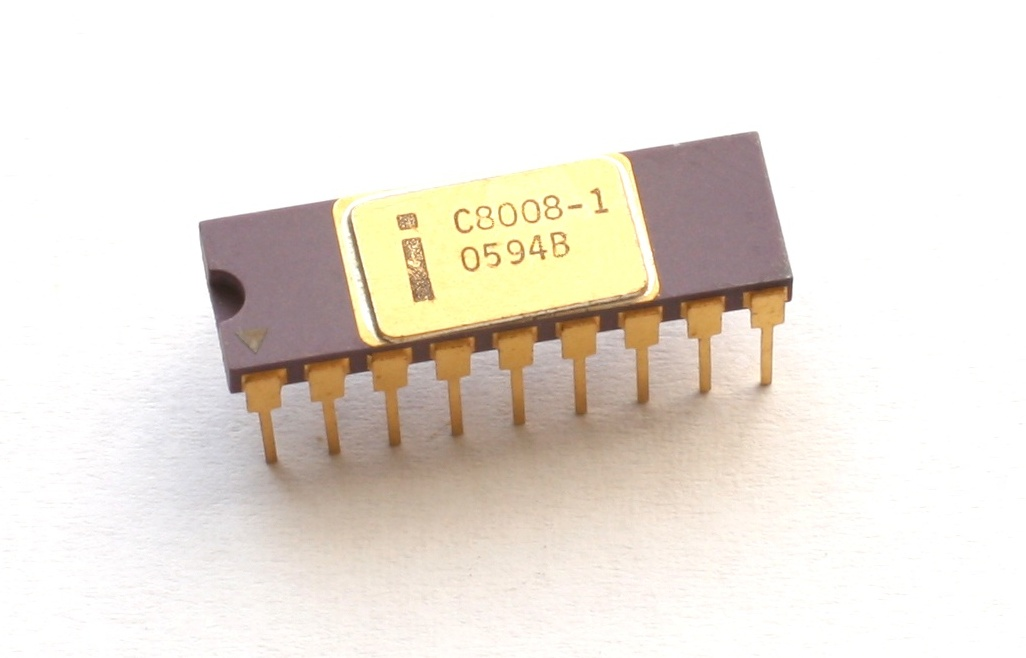
\includegraphics[width=0.8\textwidth]{images/front_Intel_C8008-1.jpg}\par
\vspace{0.5cm}

\vfill
\end{titlepage}

\clearpage

\renewcommand*\contentsname{Innehållsförteckning}
{
\setcounter{tocdepth}{2}
\tableofcontents
}

\mainmatter
\bookmarksetup{startatroot}

\chapter*{Förord}\label{fuxf6rord}
\addcontentsline{toc}{chapter}{Förord}

\markboth{Förord}{Förord}

\begin{quote}
``Det finns 10 olika typer av människor. De som förstår binära tal och
de som inte förstår.''\\
--- \emph{Okänd}
\end{quote}

Välkommen till denna kursbok i digitalteknik! Boken används som
kurslitteratur i kursen Digitalteknik på Yrkeshögskolan Yrgo, Göteborg
och utbildningarna till Elektronikingenjör. Den är skriven i Pandoc
Markdown i verktyget Visual Studio Code med tillägget Quarto för
rendering. Som stöd i skrivandet har AI använts, främst Gemini 3 Flash
men även ChatGPT GPT-5.3.

Du hittar källkoden till denna kursbok på
\href{https://github.com/yrgohenhal/Digitalteknik-Kursbok}{GitHub}.

Kursboken är fri att använda under licensen
\href{https://creativecommons.org/licenses/by-sa/4.0/}{Creative Commons
Attribution-ShareAlike 4.0 International (CC BY-SA 4.0)}.

Bildmaterial är skapat av författaren, alternativt kommer från
Wikipedia. I det senare fallet står upphovsperson och vilken Crative
Commons-licens som är aktuell i figurtexten.

Kretsscheman är skapade i Kicad 9.0.

Karnaughdiagram är skapade med onlineverktyget
\href{https://karnaughmapsolver.com/}{Karnaugh Map (K-Map) Solver}.

Titelbladet visar ett fotografi på Intel 8008. Källa: Av Konstantin
Lanzet - CPU Collection Konstantin LanzetCamera: Canon EOS 400D, CC
BY-SA 4.0, https://commons.wikimedia.org/w/index.php?curid=5694177

\bookmarksetup{startatroot}

\chapter{Introduktion}\label{introduktion}

Digitaltekniken är fundamentet för det moderna samhället. Genom att
representera information som diskreta tillstånd -- oftast som binära
värden \(0\) och \(1\) -- har vi skapat system som kan hantera data med
hög precision.

\section{Historisk bakgrund}\label{historisk-bakgrund}

\begin{itemize}
\tightlist
\item
  \textbf{George Boole:} Lade grunden för boolesk algebra på 1800-talet.
\item
  \textbf{Radiorör:} Användes i tidiga datorer som ENIAC.
\item
  \textbf{Transistorn (1947):} Den elektroniska strömbrytare som
  möjliggjorde dagens miniatyrisering.
\end{itemize}

\section{Varför digitalteknik?}\label{varfuxf6r-digitalteknik}

{\def\LTcaptype{none} % do not increment counter
\begin{longtable}[]{@{}lll@{}}
\toprule\noalign{}
Egenskap & Analog teknik & Digital teknik \\
\midrule\noalign{}
\endhead
\bottomrule\noalign{}
\endlastfoot
\textbf{Störningskänslighet} & Hög & Låg \\
\textbf{Lagring} & Degradera över tid & Förlustfri \\
\textbf{Flexibilitet} & Hårdvarubunden & Programvarubunden \\
\end{longtable}
}

Digitala system bygger på förmågan att tolka spänningsnivåer som logiska
värden. När bara två spänningsnivåer (låg och hög) ska tolkas jämfört
med analogtekniken där kontinuerliga spänningar ska hanteras, skapas en
robust elektronik!

\bookmarksetup{startatroot}

\chapter{Talsystem och aritmetik för binära
tal}\label{talsystem-och-aritmetik-fuxf6r-binuxe4ra-tal}

\section{Positionssystemet}\label{positionssystemet}

I ett positionssystem beror en siffras värde på dess position i talet.
För ett tal \(N\) med basen \(b\) kan vi uttrycka värdet som en summa av
siffror multiplicerade med basens potenser:

\[N = d_n b^n + \dots + d_1 b^1 + d_0 b^0\]

Där \(b\) är basen, \(d\) är siffran på positionen och \(n\) är
positionens exponent.

\begin{tcolorbox}[enhanced jigsaw, arc=.35mm, bottomrule=.15mm, bottomtitle=1mm, breakable, colback=white, colbacktitle=quarto-callout-note-color!10!white, colframe=quarto-callout-note-color-frame, coltitle=black, left=2mm, leftrule=.75mm, opacityback=0, opacitybacktitle=0.6, rightrule=.15mm, title=\textcolor{quarto-callout-note-color}{\faInfo}\hspace{0.5em}{Exempel: Positionssystemet för talet 432}, titlerule=0mm, toprule=.15mm, toptitle=1mm]

För att förstå hur systemet fungerar kan vi bryta ner det decimala
heltalet \textbf{432} (där \(b=10\)):

\begin{itemize}
\tightlist
\item
  Siffran \textbf{4} står på positionen \(10^2\) (hundratal):
  \(4 \cdot 10^2 = 4 \cdot 100 = 400\)
\item
  Siffran \textbf{3} står på positionen \(10^1\) (tiotal):
  \(3 \cdot 10^1 = 3 \cdot 10 = 30\)
\item
  Siffran \textbf{2} står på positionen \(10^0\) (ental):
  \(2 \cdot 10^0 = 2 \cdot 1 = 2\)
\end{itemize}

Summerat blir detta: \[400 + 30 + 2 = 432_{10}\]

\end{tcolorbox}

Positionssystemets verkliga styrka är dess abstraktion. Att vi valt att
använda basen 10 i vardagen är en biologisk slump (vi har tio fingrar),
men matematiskt är systemet helt basoberoende. Inom digitaltekniken
används binära tal (bas 2), vilket är den minsta möjliga basen för ett
positionssystem. Detta är fundamentalt eftersom digitala kretsar består
av miljarder transistorer som fungerar som strömbrytare -- det är
elektriskt säkrare att särskilja mellan två tillstånd (0 och 1) än tio.

\begin{tcolorbox}[enhanced jigsaw, arc=.35mm, bottomrule=.15mm, bottomtitle=1mm, breakable, colback=white, colbacktitle=quarto-callout-note-color!10!white, colframe=quarto-callout-note-color-frame, coltitle=black, left=2mm, leftrule=.75mm, opacityback=0, opacitybacktitle=0.6, rightrule=.15mm, title=\textcolor{quarto-callout-note-color}{\faInfo}\hspace{0.5em}{Exempel: Uppbyggnaden av talet 432 i binär form}, titlerule=0mm, toprule=.15mm, toptitle=1mm]

Om vi skriver det decimala talet \textbf{432} som ett binärt tal, ser
det ut så här:

\[432_{10} = 110110000_2\]

För att förstå hur detta tal är uppbyggt behöver vi bara placera ut våra
``bitar'' på deras respektive platser (potenser av 2). Varje \textbf{1}
representerar att den potensen ingår i summan, medan \textbf{0} betyder
att den utelämnas:

{\def\LTcaptype{none} % do not increment counter
\begin{longtable}[]{@{}
  >{\centering\arraybackslash}p{(\linewidth - 18\tabcolsep) * \real{0.1000}}
  >{\centering\arraybackslash}p{(\linewidth - 18\tabcolsep) * \real{0.1000}}
  >{\centering\arraybackslash}p{(\linewidth - 18\tabcolsep) * \real{0.1000}}
  >{\centering\arraybackslash}p{(\linewidth - 18\tabcolsep) * \real{0.1000}}
  >{\centering\arraybackslash}p{(\linewidth - 18\tabcolsep) * \real{0.1000}}
  >{\centering\arraybackslash}p{(\linewidth - 18\tabcolsep) * \real{0.1000}}
  >{\centering\arraybackslash}p{(\linewidth - 18\tabcolsep) * \real{0.1000}}
  >{\centering\arraybackslash}p{(\linewidth - 18\tabcolsep) * \real{0.1000}}
  >{\centering\arraybackslash}p{(\linewidth - 18\tabcolsep) * \real{0.1000}}
  >{\centering\arraybackslash}p{(\linewidth - 18\tabcolsep) * \real{0.1000}}@{}}
\toprule\noalign{}
\begin{minipage}[b]{\linewidth}\centering
Position (\(2^n\))
\end{minipage} & \begin{minipage}[b]{\linewidth}\centering
\(2^8\)
\end{minipage} & \begin{minipage}[b]{\linewidth}\centering
\(2^7\)
\end{minipage} & \begin{minipage}[b]{\linewidth}\centering
\(2^6\)
\end{minipage} & \begin{minipage}[b]{\linewidth}\centering
\(2^5\)
\end{minipage} & \begin{minipage}[b]{\linewidth}\centering
\(2^4\)
\end{minipage} & \begin{minipage}[b]{\linewidth}\centering
\(2^3\)
\end{minipage} & \begin{minipage}[b]{\linewidth}\centering
\(2^2\)
\end{minipage} & \begin{minipage}[b]{\linewidth}\centering
\(2^1\)
\end{minipage} & \begin{minipage}[b]{\linewidth}\centering
\(2^0\)
\end{minipage} \\
\midrule\noalign{}
\endhead
\bottomrule\noalign{}
\endlastfoot
\textbf{Värde} & 256 & 128 & 64 & 32 & 16 & 8 & 4 & 2 & 1 \\
\textbf{Bit} & \textbf{1} & \textbf{1} & \textbf{0} & \textbf{1} &
\textbf{1} & \textbf{0} & \textbf{0} & \textbf{0} & \textbf{0} \\
\end{longtable}
}

\textbf{Vi kan nu kontrollera att summan stämmer:}
\[(1 \cdot 256) + (1 \cdot 128) + (0 \cdot 64) + (1 \cdot 32) + (1 \cdot 16) + (0 \cdot 8) + (0 \cdot 4) + (0 \cdot 2) + (0 \cdot 1) = 432_{10}\]

\end{tcolorbox}

Heltal är bara en delmängd av alla tal. I det mer generella fallet med
decimaltal kan ett tal \(N\) med basen \(b\) uttryckas med hjälp av
negativa exponenter:

\[N = d_n b^n + \dots + d_0 b^0 + d_{-1} b^{-1} + d_{-2} b^{-2} + \dots\]

I Sverige används kommatecken (,) för att skilja heltalsdelen från
decimaldelen. I många andra länder används istället punkt (.) som
decimaltecken. De flesta relevanta standarder tillåter båda typerna av
tecken, så länge man är konsekvent i dokumentation. Notera att mycket
amerikansk litteratur använder punkt som decimaltecken och komma som
tusenavskiljare, t.ex. så skrivs talet \(12345,67\) som \(12,345.67\).

\begin{tcolorbox}[enhanced jigsaw, arc=.35mm, bottomrule=.15mm, bottomtitle=1mm, breakable, colback=white, colbacktitle=quarto-callout-note-color!10!white, colframe=quarto-callout-note-color-frame, coltitle=black, left=2mm, leftrule=.75mm, opacityback=0, opacitybacktitle=0.6, rightrule=.15mm, title=\textcolor{quarto-callout-note-color}{\faInfo}\hspace{0.5em}{Exempel: Positionssystemet för 432,57}, titlerule=0mm, toprule=.15mm, toptitle=1mm]

Låt oss bryta ner det decimala talet \textbf{432,57} (\(b=10\)):

\textbf{Heltalsdel:}
\(4 \cdot 10^2 + 3 \cdot 10^1 + 2 \cdot 10^0 = 400 + 30 + 2 = 432\)

\textbf{Decimaldel:}
\(5 \cdot 10^{-1} + 7 \cdot 10^{-2} = 0,5 + 0,07 = 0,57\)

Summerat: \(432 + 0,57 = 432,57_{10}\)

\end{tcolorbox}

I det binära systemet (\(b=2\)) fungerar ``binärpunkten'' på samma sätt.
Positionerna till höger om punkten representerar negativa potenser av 2:

\begin{itemize}
\tightlist
\item
  \(2^{-1} = 0,5\)
\item
  \(2^{-2} = 0,25\)
\item
  \(2^{-3} = 0,125\)
\end{itemize}

Det binära systemet har en inneboende begränsning när det gäller att
representera decimaltal exakt. Precis som att vissa bråk i det decimala
systemet får en oändlig periodisk decimalutveckling (t.ex.
\(1/3 \approx 0,333...\)), kan många enkla decimaltal inte representeras
med ett ändligt antal binära bitar.

För att hantera detta används i datorer en standard som kallas
\textbf{flyttal}. Istället för en fast punkt lagrar datorn talet som en
\textbf{signifikand} (själva talvärdet) och en \textbf{exponent} (som
anger var punkten ska placeras). Detta gör att vi kan representera både
extremt stora och extremt små tal, men med en kompromiss: vi får en
begränsad \textbf{precision}. När talet inte går att uttrycka exakt med
de tillgängliga bitarna sker en avrundning, vilket är viktigt att känna
till vid känsliga beräkningar.

\section{Decimala, binära och hexadecimala
systemet}\label{decimala-binuxe4ra-och-hexadecimala-systemet}

I digitaltekniken arbetar vi främst med tre talsystem som var och en
tjänar ett specifikt syfte:

\begin{itemize}
\tightlist
\item
  \textbf{Decimalt (bas 10):} Vår vardagsmatematik. Används främst för
  kommunikation mellan människa och maskin (input/output).
\item
  \textbf{Binärt (bas 2):} Grunden för all digital elektronik.
\item
  \textbf{Hexadecimalt (bas 16):} Ett kompakt sätt att representera
  binära data. Eftersom en binär sträng snabbt blir svårläst för en
  människa (t.ex. \(11101011_2\)), grupperar vi bitarna för att skapa
  hexadecimala tecken (\(0-9, A-F\)).
\end{itemize}

\subsection{Binära tal och logik}\label{binuxe4ra-tal-och-logik}

Kärnan i det binära systemet är att det mappar perfekt mot logikens
värld. I en digital krets representerar vi talen som spänningsnivåer.
Detta översätts direkt till \textbf{boolesk logik}, där:

\begin{itemize}
\tightlist
\item
  \textbf{1} motsvarar ``Sant'' (High/On, t.ex. 5V).
\item
  \textbf{0} motsvarar ``Falskt'' (Low/Off, t.ex. 0V).
\end{itemize}

Detta gör att varje binär siffra (bit) blir en logisk variabel, vilket
är fundamentet för hur datorns processorer bygger upp komplexa beslut
genom enkla grindar som AND, OR och NOT.

\subsection{Index-notering för
talbaser}\label{index-notering-fuxf6r-talbaser}

För att undvika missförstånd när vi blandar olika talsystem i samma
text, använder vi ett \textbf{index} (subscript). Talbasen skrivs som
ett litet tal efter själva värdet:

\begin{itemize}
\tightlist
\item
  \(234_{10}\) betyder talet 234 i bas 10.
\item
  \(11101010_2\) betyder ett binärt tal.
\item
  \(EA_{16}\) betyder ett hexadecimalt tal.
\end{itemize}

Nedan presenteras en jämförelse av hur talen 0 till 15 representeras i
de tre vanligaste talsystemen inom digitalteknik.

\begin{longtable}[]{@{}lll@{}}
\caption{Jämförelse av talsystem
(0--15)}\label{tbl-talsystem}\tabularnewline
\toprule\noalign{}
Decimalt & Binärt & Hexadecimalt \\
\midrule\noalign{}
\endfirsthead
\toprule\noalign{}
Decimalt & Binärt & Hexadecimalt \\
\midrule\noalign{}
\endhead
\bottomrule\noalign{}
\endlastfoot
0 & 0000 & 0 \\
1 & 0001 & 1 \\
2 & 0010 & 2 \\
3 & 0011 & 3 \\
4 & 0100 & 4 \\
5 & 0101 & 5 \\
6 & 0110 & 6 \\
7 & 0111 & 7 \\
8 & 1000 & 8 \\
9 & 1001 & 9 \\
10 & 1010 & A \\
11 & 1011 & B \\
12 & 1100 & C \\
13 & 1101 & D \\
14 & 1110 & E \\
15 & 1111 & F \\
\end{longtable}

Som framgår av Tabell~\ref{tbl-talsystem} motsvarar en enda hexadecimal
siffra (0--F) exakt fyra binära bitar. Denna gruppering, ofta kallad en
``nibble'', är anledningen till att hexadecimal form är så effektiv för
att representera binära data.

\begin{tcolorbox}[enhanced jigsaw, arc=.35mm, bottomrule=.15mm, bottomtitle=1mm, breakable, colback=white, colbacktitle=quarto-callout-note-color!10!white, colframe=quarto-callout-note-color-frame, coltitle=black, left=2mm, leftrule=.75mm, opacityback=0, opacitybacktitle=0.6, rightrule=.15mm, title=\textcolor{quarto-callout-note-color}{\faInfo}\hspace{0.5em}{Exempel: Talet 234 i olika system}, titlerule=0mm, toprule=.15mm, toptitle=1mm]

Låt oss se hur det decimala talet \textbf{234} representeras i de tre
vanligaste systemen:

{\def\LTcaptype{none} % do not increment counter
\begin{longtable}[]{@{}ll@{}}
\toprule\noalign{}
System & Representation \\
\midrule\noalign{}
\endhead
\bottomrule\noalign{}
\endlastfoot
\textbf{Decimalt} & \(234_{10}\) \\
\textbf{Binärt} & \(11101010_2\) \\
\textbf{Hexadecimalt} & \(EA_{16}\) \\
\end{longtable}
}

\textbf{Kort förklaring:}

\begin{itemize}
\tightlist
\item
  \textbf{Decimalt:} Vårt vanliga sätt att räkna.
\item
  \textbf{Binärt:} \(128 + 64 + 32 + 8 + 2 = 234\).
\item
  \textbf{Hexadecimalt:} \(E\) (som är 14) gånger \(16^1\) plus \(A\)
  (som är 10) gånger \(16^0\) ger \(224 + 10 = 174\).
\end{itemize}

\end{tcolorbox}

\subsection{Bit, nibble och byte?}\label{bit-nibble-och-byte}

Inom digitaltekniken grupperar vi binära siffror för att kunna hantera
komplex information effektivare. Här är de grundläggande enheterna vi
använder:

\begin{itemize}
\tightlist
\item
  \textbf{Bit (Binary Digit):} Den minsta informationsenheten. En bit
  kan anta värdet 0 eller 1 och motsvarar ett logiskt tillstånd
  (sant/falskt).
\item
  \textbf{Nibble:} En grupp om \textbf{4 bitar}. En nibble kan
  representera 16 olika värden (\(2^4\)), vilket gör att den motsvarar
  exakt ett hexadecimalt tecken (0--F).
\item
  \textbf{Byte:} En grupp om \textbf{8 bitar}. Byten är den
  standardiserade grundenheten för nästan all datalagring och
  minnesadressering. En byte kan representera \(2^8 = 256\) unika
  kombinationer.
\item
  \textbf{Word:} Storleken på ett ``ord'' varierar beroende på
  arkitektur (t.ex. 16, 32 eller 64 bitar) och representerar den mängd
  data som processorn kan bearbeta i en enda operation.
\end{itemize}

Genom att använda Tabell~\ref{tbl-talsystem} kan vi se att en nibble är
bryggan mellan det binära systemet och den mer läsbara hexadecimala
notationen. När vi arbetar med minnesadresser eller register i en
processor, används nästan uteslutande att tala i termer av bytes och
ordlängder.

I en historisk kontext hittar vi anledningen till att vi ofta grupperar
bitar i 4, 8, 16 osv. Det skapar en direkt matematisk koppling till både
det hexadecimala talsystemet och datorns minnesstruktur. Utvecklingen av
datorarkitekturer har varit en ständig kamp mellan behovet av mer
beräkningskraft och de fysiska begränsningarna i kisel.

\begin{itemize}
\tightlist
\item
  \textbf{Intel 4004 (1971):} Världens första kommersiellt tillgängliga
  mikroprocessor. Det var en \textbf{4-bitars processor}, vilket innebär
  att dess ``ordlängd'' var precis en \textbf{nibble}. Den var primärt
  designad för miniräknare och kunde adressera en mycket begränsad mängd
  minne.
\item
  \textbf{Intel 8008 \& 8080 (1972/1974):} Tog steget till
  \textbf{8-bitars arkitektur}. Här blev \textbf{byten} den naturliga
  standarden för datalagring, vilket vi fortfarande lever med idag. Det
  gjorde det möjligt att hantera tecken (ASCII) och mer komplexa
  instruktionsuppsättningar.
\item
  \textbf{16- till 64-bitar:} Under 80- och 90-talen skedde en snabb
  utveckling där ordlängden fördubblades med jämna mellanrum för att
  kunna hantera större minnesadresser (RAM) och mer komplexa datatyper
  som flyttal.
\end{itemize}

När vi idag pratar om ``32-bitars'' eller ``64-bitars'' operativsystem,
refererar vi direkt till hur stor den interna ordlängden i processorn
är. En 64-bitars processor kan hantera astronomiska mängder
minnesadresser (\(2^{64}\) stycken), vilket var helt otänkbart för
ingenjörerna bakom Intel 4004.

\subsection{MSB och LSB: Bitarnas vikt}\label{msb-och-lsb-bitarnas-vikt}

I ett positionssystem har varje position i ett tal ett specifikt
``värde'' (vikt). Precis som att siffran längst till vänster i ett
decimalt tal (t.ex. ``4'' i 432) representerar det största värdet
(hundratal), har vi motsvarande begrepp för binära tal för att
identifiera vilken bit som bär mest respektive minst information.

\begin{itemize}
\tightlist
\item
  \textbf{MSB (Most Significant Bit):} Den ``mest signifikanta biten''.
  Detta är biten som har högst vikt, det vill säga den bit som står
  längst till vänster i talet. Den har störst påverkan på talets totala
  värde.
\item
  \textbf{LSB (Least Significant Bit):} Den ``minst signifikanta
  biten''. Detta är biten med lägst vikt, som står längst till höger
  (entalspositionen). Den avgör bara om talet är jämnt (0) eller udda
  (1).
\end{itemize}

\begin{tcolorbox}[enhanced jigsaw, arc=.35mm, bottomrule=.15mm, bottomtitle=1mm, breakable, colback=white, colbacktitle=quarto-callout-note-color!10!white, colframe=quarto-callout-note-color-frame, coltitle=black, left=2mm, leftrule=.75mm, opacityback=0, opacitybacktitle=0.6, rightrule=.15mm, title=\textcolor{quarto-callout-note-color}{\faInfo}\hspace{0.5em}{Exempel: Viktning av bitar i talet \(1101_2\)}, titlerule=0mm, toprule=.15mm, toptitle=1mm]

I det binära talet \textbf{\(1101_2\)} ser vi tydligt hur vikten
fördelas:

{\def\LTcaptype{none} % do not increment counter
\begin{longtable}[]{@{}lcccc@{}}
\toprule\noalign{}
Position & \(2^3\) (8) & \(2^2\) (4) & \(2^1\) (2) & \(2^0\) (1) \\
\midrule\noalign{}
\endhead
\bottomrule\noalign{}
\endlastfoot
\textbf{Bit} & \textbf{1} & 1 & 0 & \textbf{1} \\
\textbf{Betydelse} & \textbf{MSB} & & & \textbf{LSB} \\
\end{longtable}
}

\begin{itemize}
\tightlist
\item
  \textbf{MSB} har vikten \(2^3 = 8\). Ändras denna bit, ändras talets
  värde med 8.
\item
  \textbf{LSB} har vikten \(2^0 = 1\). Ändras denna bit, ändras talets
  värde bara med 1.
\end{itemize}

\end{tcolorbox}

Att förstå vilken bit som är MSB och vilken som är LSB är fundamentalt
för hur processorer hanterar data. Det är avgörande för det som kallas
\textbf{Endian} (i vilken ordning bytes lagras i minnet eller ordningen
bitar skickas i seriell kommunikation) och när vi utför logiska
skiftoperationer, där vi antingen ``skiftar ut'' MSB eller LSB för att
manipulera talets storlek eller tecken.

\section{Konverteringar mellan
talsystem}\label{konverteringar-mellan-talsystem}

Att kunna konvertera mellan talsystem är en fundamental färdighet för
att förstå hur data flyttas och tolkas i en dator.

\subsection{\texorpdfstring{Decimalt \(\leftrightarrow\)
Binärt}{Decimalt \textbackslash leftrightarrow Binärt}}\label{decimalt-leftrightarrow-binuxe4rt}

\subsubsection{Decimalt till binärt (Division med
2)}\label{decimalt-till-binuxe4rt-division-med-2}

Metoden går ut på att upprepade gånger dividera talet med 2 och notera
resten. Vi läser sedan resterna nerifrån och upp. Det kan vara
förvirrande att första divisionen med \$\(/ 2\) ger LSB och den sista
ger MSB. Men första divisionen talar om huruvida det binära talet är
jämnt eller udda, vilket motsvarar den bit som har vikten \(2^0\) och
positionen \(0\). Sista divisionen indikerar hur stort talet är. Förr
eller senare kommer divisionen ge svaret \(0\), och när det händer så
har vi kommit till den bit som har den högsta positionen \(2^n\). Det
motsvarar då MSB.

\begin{tcolorbox}[enhanced jigsaw, arc=.35mm, bottomrule=.15mm, bottomtitle=1mm, breakable, colback=white, colbacktitle=quarto-callout-note-color!10!white, colframe=quarto-callout-note-color-frame, coltitle=black, left=2mm, leftrule=.75mm, opacityback=0, opacitybacktitle=0.6, rightrule=.15mm, title=\textcolor{quarto-callout-note-color}{\faInfo}\hspace{0.5em}{Exempel: Omvandla \(13_{10}\) till binärt}, titlerule=0mm, toprule=.15mm, toptitle=1mm]

\begin{enumerate}
\def\labelenumi{\arabic{enumi}.}
\tightlist
\item
  \(13 / 2 = 6\) med rest \textbf{1} (LSB)
\item
  \(6 / 2 = 3\) med rest \textbf{0}
\item
  \(3 / 2 = 1\) med rest \textbf{1}
\item
  \(1 / 2 = 0\) med rest \textbf{1} (MSB)
\end{enumerate}

Läst nerifrån och upp får vi: \(1101_2\).

\end{tcolorbox}

\subsubsection{Binärt till decimalt (Positionell
summering)}\label{binuxe4rt-till-decimalt-positionell-summering}

Här multiplicerar vi varje bit med dess tillhörande potens av 2 och
summerar resultaten.

\begin{tcolorbox}[enhanced jigsaw, arc=.35mm, bottomrule=.15mm, bottomtitle=1mm, breakable, colback=white, colbacktitle=quarto-callout-note-color!10!white, colframe=quarto-callout-note-color-frame, coltitle=black, left=2mm, leftrule=.75mm, opacityback=0, opacitybacktitle=0.6, rightrule=.15mm, title=\textcolor{quarto-callout-note-color}{\faInfo}\hspace{0.5em}{Exempel: Omvandla \(1011_2\) till decimalt}, titlerule=0mm, toprule=.15mm, toptitle=1mm]

\((1 \cdot 2^3) + (0 \cdot 2^2) + (1 \cdot 2^1) + (1 \cdot 2^0)\)
\(= 8 + 0 + 2 + 1 = 11_{10}\)

\end{tcolorbox}

\subsection{\texorpdfstring{Binärt \(\leftrightarrow\)
Hexadecimalt}{Binärt \textbackslash leftrightarrow Hexadecimalt}}\label{binuxe4rt-leftrightarrow-hexadecimalt}

Det hexadecimala systemet är effektivt att skriva jämfört med det binära
eftersom \(16 = 2^4\). Det betyder att exakt fyra binära bitar motsvarar
en hexadecimal siffra.

\subsubsection{Binärt till hexadecimalt
(Gruppering)}\label{binuxe4rt-till-hexadecimalt-gruppering}

Dela upp den binära strängen i grupper om 4 bitar, räknat från höger
(LSB).

\begin{tcolorbox}[enhanced jigsaw, arc=.35mm, bottomrule=.15mm, bottomtitle=1mm, breakable, colback=white, colbacktitle=quarto-callout-note-color!10!white, colframe=quarto-callout-note-color-frame, coltitle=black, left=2mm, leftrule=.75mm, opacityback=0, opacitybacktitle=0.6, rightrule=.15mm, title=\textcolor{quarto-callout-note-color}{\faInfo}\hspace{0.5em}{Exempel: Omvandla \(111101_2\) till hexadecimalt}, titlerule=0mm, toprule=.15mm, toptitle=1mm]

\begin{enumerate}
\def\labelenumi{\arabic{enumi}.}
\tightlist
\item
  Gruppering: \(0011\) \textbar{} \(1101\) (två extra nollor läggs till
  i början för att ge en full nibble)
\item
  Omvandla varje grupp: \(3\) \textbar{} \(D\)
\end{enumerate}

Resultat: \(3D_{16}\)

\end{tcolorbox}

\subsubsection{Hexadecimalt till binärt
(Expansion)}\label{hexadecimalt-till-binuxe4rt-expansion}

Varje hexadecimalt tecken översätts direkt till dess 4-bitars binära
motsvarighet.

\begin{tcolorbox}[enhanced jigsaw, arc=.35mm, bottomrule=.15mm, bottomtitle=1mm, breakable, colback=white, colbacktitle=quarto-callout-note-color!10!white, colframe=quarto-callout-note-color-frame, coltitle=black, left=2mm, leftrule=.75mm, opacityback=0, opacitybacktitle=0.6, rightrule=.15mm, title=\textcolor{quarto-callout-note-color}{\faInfo}\hspace{0.5em}{Exempel: Omvandla \(A5_{16}\) till binärt}, titlerule=0mm, toprule=.15mm, toptitle=1mm]

\begin{enumerate}
\def\labelenumi{\arabic{enumi}.}
\tightlist
\item
  \(A = 1010\)
\item
  \(5 = 0101\)
\end{enumerate}

Resultat: \(10100101_2\)

\end{tcolorbox}

Som framgår av \textbf{Tabell~\ref{tbl-talsystem}} är nibble-strukturen
(4 bitar) nyckeln till enkel konvertering mellan binära och hexadecimala
tal.

\subsection{Binär aritmetik}\label{binuxe4r-aritmetik}

Binär aritmetik bygger på samma principer som decimal räkning, men med
en mycket begränsad sifferuppsättning (0 och 1), vilket gör den idealisk
för digitala kretsar.

\subsection{Addition och subtraktion}\label{addition-och-subtraktion}

Addition utförs kolumnvis från höger till vänster. En ``minnessiffra''
(carry) uppstår när summan i en kolumn blir 2 eller mer
(\(1+1 = 10_2\)). Denna carry förs över till nästa kolumn till vänster.

\begin{tcolorbox}[enhanced jigsaw, arc=.35mm, bottomrule=.15mm, bottomtitle=1mm, breakable, colback=white, colbacktitle=quarto-callout-note-color!10!white, colframe=quarto-callout-note-color-frame, coltitle=black, left=2mm, leftrule=.75mm, opacityback=0, opacitybacktitle=0.6, rightrule=.15mm, title=\textcolor{quarto-callout-note-color}{\faInfo}\hspace{0.5em}{Exempel: Binär addition (\(7_{10} + 5_{10}\))}, titlerule=0mm, toprule=.15mm, toptitle=1mm]

För att tydliggöra \emph{carry} (minnessiffror) ställer vi upp talen i
kolumner:

\[
\begin{array}{r@{\quad}c@{\,}c@{\,}c@{\,}c@{\quad}l}
  \text{Carry:} & \color{red}{\phantom{1}} & \color{red}{1} & \color{red}{1} & \color{red}{\phantom{1}} & \\[-0.5ex]
  & 0 & 1 & 1 & 1_2 & (7_{10}) \\
+ & 0 & 1 & 0 & 1_2 & (5_{10}) \\
\hline
  & 1 & 1 & 0 & 0_2 & (12_{10})
\end{array}
\]

\textbf{Förklaring:} I varje kolumn där summan överstiger \(1\), skickas
en \(\color{red}{1}\) (carry) till nästa kolumn till vänster.

\end{tcolorbox}

Subtraktion hanteras enklast genom att låna från nästa högre position
(borrow), på samma sätt som i decimal subtraktion.

\begin{tcolorbox}[enhanced jigsaw, arc=.35mm, bottomrule=.15mm, bottomtitle=1mm, breakable, colback=white, colbacktitle=quarto-callout-note-color!10!white, colframe=quarto-callout-note-color-frame, coltitle=black, left=2mm, leftrule=.75mm, opacityback=0, opacitybacktitle=0.6, rightrule=.15mm, title=\textcolor{quarto-callout-note-color}{\faInfo}\hspace{0.5em}{Exempel: Binär subtraktion med lån (\(6_{10} - 1_{10}\))}, titlerule=0mm, toprule=.15mm, toptitle=1mm]

När vi lånar i det binära talsystemet lånar vi alltid värdet \(2_{10}\),
vilket binärt skrivs som \(10_2\).

\[
\begin{array}{r@{\quad}c@{\,}c@{\,}c@{\,}c@{\quad}l}
  \text{Lån:} & & & & \color{red}{\scriptstyle 10} & \\[-0.8ex]
  & 0 & 1 & \cancel{1} & 0_2 & (6_{10}) \\
- & 0 & 0 & 0 & 1_2 & (1_{10}) \\
\hline
  & 0 & 1 & 0 & 1_2 & (5_{10})
\end{array}
\]

\textbf{Förklaring:}

\begin{enumerate}
\def\labelenumi{\arabic{enumi}.}
\tightlist
\item
  I kolumnen längst till höger kan vi inte ta \(0-1\).
\item
  Vi lånar från nästa kolumn, stryker dess etta (\(\cancel{1}\)) och
  flyttar lånet ett steg till höger. Lånet landar som en röd
  \(\color{red}{10}\) ovanför nollan längst till höger.
\end{enumerate}

\end{tcolorbox}

\subsection{Multiplikation och
division}\label{multiplikation-och-division}

Att multiplicera eller dividera med heltal som är potenser av \(2^n\) är
extremt effektivt genom att använda bit-skiftningar.

\begin{tcolorbox}[enhanced jigsaw, arc=.35mm, bottomrule=.15mm, bottomtitle=1mm, breakable, colback=white, colbacktitle=quarto-callout-note-color!10!white, colframe=quarto-callout-note-color-frame, coltitle=black, left=2mm, leftrule=.75mm, opacityback=0, opacitybacktitle=0.6, rightrule=.15mm, title=\textcolor{quarto-callout-note-color}{\faInfo}\hspace{0.5em}{Exempel: Vänsterskift (Multiplikation med 2)}, titlerule=0mm, toprule=.15mm, toptitle=1mm]

\[
\begin{array}{r@{\quad}l}
  \text{Innan:} & 0011_2 \quad (3_{10}) \\
  \text{Skift:} & \leftarrow 1 \\
  \hline
  \text{Efter:} & 0110_2 \quad (6_{10})
\end{array}
\] \(\Rightarrow\) \textbf{Förklaring:} Varje bit flyttas ett steg till
vänster, vilket fördubblar dess vikt (\(2^0\) blir \(2^1\) osv).

\end{tcolorbox}

\begin{tcolorbox}[enhanced jigsaw, arc=.35mm, bottomrule=.15mm, bottomtitle=1mm, breakable, colback=white, colbacktitle=quarto-callout-note-color!10!white, colframe=quarto-callout-note-color-frame, coltitle=black, left=2mm, leftrule=.75mm, opacityback=0, opacitybacktitle=0.6, rightrule=.15mm, title=\textcolor{quarto-callout-note-color}{\faInfo}\hspace{0.5em}{Exempel: Högerskift (Division med 2)}, titlerule=0mm, toprule=.15mm, toptitle=1mm]

\[
\begin{array}{r@{\quad}l}
  \text{Innan:} & 1010_2 \quad (10_{10}) \\
  \text{Skift:} & 1 \rightarrow \\
  \hline
  \text{Efter:} & 0101_2 \quad (5_{10})
\end{array}
\] \(\Rightarrow\) \textbf{Förklaring:} Bitarna flyttas ett steg till
höger. Den minst signifikanta biten (LSB) ``faller av'' och går
förlorad.

\end{tcolorbox}

\begin{tcolorbox}[enhanced jigsaw, arc=.35mm, bottomrule=.15mm, bottomtitle=1mm, breakable, colback=white, colbacktitle=quarto-callout-note-color!10!white, colframe=quarto-callout-note-color-frame, coltitle=black, left=2mm, leftrule=.75mm, opacityback=0, opacitybacktitle=0.6, rightrule=.15mm, title=\textcolor{quarto-callout-note-color}{\faInfo}\hspace{0.5em}{Exempel: Multiplikation med 4 (\(2^2\))}, titlerule=0mm, toprule=.15mm, toptitle=1mm]

Att multiplicera med 4 motsvarar ett skift två steg åt vänster.

\[
\begin{array}{r@{\quad}l}
  \text{Tal:} & 00101100_2 \quad (44_{10}) \\
  \text{Skift 2 steg:} & \leftarrow 2 \\
  \hline
  \text{Resultat:} & 10110000_2 \quad (176_{10})
\end{array}
\]

\end{tcolorbox}

Om vi begränsat multiplikationen genom att exempelvis bara använda en
byte och hade startat med ett tal där bitar flyttas utanför det 8-bitars
fönstret som begränsar en byte, skulle dessa höga bitar gå förlorade.
Detta kallas för ett \emph{overflow}. Hårdvaran kan då inte längre
representera det korrekta värdet, vilket resulterar i ett matematiskt
fel.

\begin{tcolorbox}[enhanced jigsaw, arc=.35mm, bottomrule=.15mm, bottomtitle=1mm, breakable, colback=white, colbacktitle=quarto-callout-note-color!10!white, colframe=quarto-callout-note-color-frame, coltitle=black, left=2mm, leftrule=.75mm, opacityback=0, opacitybacktitle=0.6, rightrule=.15mm, title=\textcolor{quarto-callout-note-color}{\faInfo}\hspace{0.5em}{Exempel: Multiplikation med 8 (\(2^3\)) och overflow}, titlerule=0mm, toprule=.15mm, toptitle=1mm]

Att multiplicera med 8 motsvarar ett skift tre steg åt vänster. Här
kommer detta leda till \emph{overflow}.

\[
\begin{array}{r@{\quad}l}
  \text{Tal:} & 00101100_2 \quad (44_{10}) \\
  \text{Skift 3 steg:} & \leftarrow 3 \\
  \hline
  \text{Resultat:} & \textcolor{red}{1}\textcolor{black}{01100000}_2 \quad (\text{tolkas som } 96_{10} \text{ och inte } 352_{10})
\end{array}
\]

Här ger multiplikationen alltså ett fel när MSB går förlorad i overflow.

\end{tcolorbox}

Metodiken som beskrivits ovan för addition, subtraktion, multiplikation
och division fungerar även decimaltal, men begränsningen vid
multiplikation och division är att multiplikator respektive divisor är
ett heltal baserat på faktor 2. Vid allmän multiplikation/division med
godtyckliga tal krävs mer komplexa algoritmer där man iterativt även
utför addition eller subtraktion. Division är den mest resurskrävande
operationen och tar betydligt fler klockcykler i en processor än en
enkel addition.

\section{Hantering av negativa tal}\label{hantering-av-negativa-tal}

För att representera negativa tal i datorer används olika metoder för
att möjliggöra effektiv aritmetik. Här går vi igenom de vanligaste
sätten. Vi inleder med unsigned, som inte kan hantera negativa tal men
är en start för att visa olika sätt att hantera negativa tal inom
digitaltekniken. Här begränsas exemplen till 8-bitars tal, men de gäller
generellt.

\subsection{Unsigned (Osignerade tal)}\label{unsigned-osignerade-tal}

Alla bitar används för att representera positiva värden. En byte kan då
representera talen \(0\) till \(2^8 - 1\) (\(0\) till \(255_{10}\) eller
binärt \(11111111_2\)).

\begin{tcolorbox}[enhanced jigsaw, arc=.35mm, bottomrule=.15mm, bottomtitle=1mm, breakable, colback=white, colbacktitle=quarto-callout-note-color!10!white, colframe=quarto-callout-note-color-frame, coltitle=black, left=2mm, leftrule=.75mm, opacityback=0, opacitybacktitle=0.6, rightrule=.15mm, title=\textcolor{quarto-callout-note-color}{\faInfo}\hspace{0.5em}{Exempel: 8-bitars unsigned}, titlerule=0mm, toprule=.15mm, toptitle=1mm]

Talet \(00000101_2\) representerar:
\(1 \cdot 2^2 + 1 \cdot 2^0 = 4 + 1 = 5_{10}\).

Talet \(10000000_2\) representerar: \(1 \cdot 2^7 = 128_{10}\).

\end{tcolorbox}

\subsection{Signed (Signed-Magnitude,
Tecken-belopp)}\label{signed-signed-magnitude-tecken-belopp}

MSB (den mest signifikanta biten) används som teckenbit
(\(0 = +, 1 = -\)).

\textbf{Fördelar:}

\begin{itemize}
\tightlist
\item
  Enkelt att läsa ut talet: läs MSB som tecken och resterande 7 bitar
  som talets värde.
\item
  Enkelt att läsa absolutbeloppet genom att maskera bort MSB.
\end{itemize}

\textbf{Nackdelar:}

\begin{itemize}
\tightlist
\item
  Två representationer för noll (\(+0\) och \(-0\)).
\item
  Addition och subtraktion kräver komplex logik för att hantera
  teckenbitar separat.
\item
  Hårdvaran blir betydligt mer komplex då processorn måste kontrollera
  tecken innan beräkning.
\end{itemize}

\begin{tcolorbox}[enhanced jigsaw, arc=.35mm, bottomrule=.15mm, bottomtitle=1mm, breakable, colback=white, colbacktitle=quarto-callout-note-color!10!white, colframe=quarto-callout-note-color-frame, coltitle=black, left=2mm, leftrule=.75mm, opacityback=0, opacitybacktitle=0.6, rightrule=.15mm, title=\textcolor{quarto-callout-note-color}{\faInfo}\hspace{0.5em}{Exempel: 8-bitars Signed-Magnitude}, titlerule=0mm, toprule=.15mm, toptitle=1mm]

\begin{itemize}
\tightlist
\item
  \(+5_{10}\) blir \(00000101_2\)
\item
  \(-5_{10}\) blir \(10000101_2\)
\item
  Adderas dessa tal genom enkel addition blir resultatet
  \(00000101_2 + 10000101_2 = 10001010_2 = 138_{10}\) och inte \(0\) som
  man förväntar sig.
\item
  Talet \(10000000_2\) blir \(-0\), vilket är onödigt då det redan finns
  ett tal för \(0\).
\end{itemize}

\end{tcolorbox}

\subsection{1-komplement}\label{komplement}

I 1-komplement representeras negativa tal genom att invertera alla bitar
i det motsvarande positiva talets representation (där en ``0''-bit i
MSB-positionen indikerar ett positivt tal).

\textbf{Fördelar:}

\begin{itemize}
\tightlist
\item
  Enkelt att generera ett negativt tal genom invertering.
\end{itemize}

\textbf{Nackdelar:}

\begin{itemize}
\tightlist
\item
  \textbf{Dubbla nollor:} Det finns två representationer för noll:
  \(+0\) (\(00000000_2\)) och \(-0\) (\(11111111_2\)).
\item
  \textbf{Hårdvarukomplexitet:} Subtraktion (och addition av negativa
  tal) kräver en extra logisk operation, en så kallad \emph{end-around
  carry}, där en eventuell carry-bit från MSB måste adderas tillbaka
  till LSB-positionen.
\end{itemize}

\begin{tcolorbox}[enhanced jigsaw, arc=.35mm, bottomrule=.15mm, bottomtitle=1mm, breakable, colback=white, colbacktitle=quarto-callout-note-color!10!white, colframe=quarto-callout-note-color-frame, coltitle=black, left=2mm, leftrule=.75mm, opacityback=0, opacitybacktitle=0.6, rightrule=.15mm, title=\textcolor{quarto-callout-note-color}{\faInfo}\hspace{0.5em}{Exempel: \(5_{10} - 3_{10}\) i 8-bitars 1-komplement}, titlerule=0mm, toprule=.15mm, toptitle=1mm]

\begin{enumerate}
\def\labelenumi{\arabic{enumi}.}
\tightlist
\item
  \textbf{Konvertering:} \(5_{10} = 00000101_2\) och
  \(3_{10} = 00000011_2\).
\item
  \textbf{1-komplement:} Invertera bitarna i
  \(3_{10} \rightarrow 11111100_2\).
\item
  \textbf{Addition:}
\end{enumerate}

\[
\begin{array}{r@{\quad}l}
   00000101 & (5) \\
+  11111100 & (-3) \\
\hline
(1)00000001 & 
\end{array}
\]

\begin{enumerate}
\def\labelenumi{\arabic{enumi}.}
\setcounter{enumi}{3}
\tightlist
\item
  \textbf{End-around carry:} Addera carry-biten från MSB till LSB:
\end{enumerate}

\[
\begin{array}{r@{\quad}l}
   00000001 & \\
+  1 & \\
\hline
   00000010 & (2)
\end{array}
\]

\end{tcolorbox}

\subsection{2-komplement}\label{komplement-1}

I 2-komplement representeras negativa tal genom att man tar
1-komplementet av det positiva talet och därefter adderar 1.

\begin{tcolorbox}[enhanced jigsaw, arc=.35mm, bottomrule=.15mm, bottomtitle=1mm, breakable, colback=white, colbacktitle=quarto-callout-note-color!10!white, colframe=quarto-callout-note-color-frame, coltitle=black, left=2mm, leftrule=.75mm, opacityback=0, opacitybacktitle=0.6, rightrule=.15mm, title=\textcolor{quarto-callout-note-color}{\faInfo}\hspace{0.5em}{Exempel: \(-5_{10}\) i 8-bitars 2-komplement}, titlerule=0mm, toprule=.15mm, toptitle=1mm]

\begin{enumerate}
\def\labelenumi{\arabic{enumi}.}
\tightlist
\item
  \textbf{Positivt tal (+5):} \texttt{0000\ 0101}
\item
  \textbf{Invertera alla bitar:} \texttt{1111\ 1010}
\item
  \textbf{Addera 1:} \texttt{1111\ 1011} \textbf{Resultat:} \(-5_{10}\)
  representeras som \texttt{1111\ 1011}.
\end{enumerate}

\end{tcolorbox}

\textbf{Fördelar:}

\begin{itemize}
\tightlist
\item
  \textbf{Endast en nolla existerar:} \(00000000_2\) är \(+0\). Det
  finns ingen \(-0\).
\item
  \textbf{Effektiv hårdvara:} Subtraktion utförs genom vanlig addition,
  vilket gör att en och samma krets kan hantera både addition och
  subtraktion utan extra korrigeringssteg.
\end{itemize}

\textbf{Nackdelar:}

\begin{itemize}
\tightlist
\item
  Intervallet är asymmetriskt; det finns ett negativt tal mer än det
  finns positiva tal (för \(n\) bitar: \(-2^{n-1}\) till
  \(2^{n-1} - 1\)).
\item
  Det är svårare (som människa) att läsa ut värdet på ett negativt tal.
\end{itemize}

\begin{tcolorbox}[enhanced jigsaw, arc=.35mm, bottomrule=.15mm, bottomtitle=1mm, breakable, colback=white, colbacktitle=quarto-callout-note-color!10!white, colframe=quarto-callout-note-color-frame, coltitle=black, left=2mm, leftrule=.75mm, opacityback=0, opacitybacktitle=0.6, rightrule=.15mm, title=\textcolor{quarto-callout-note-color}{\faInfo}\hspace{0.5em}{Exempel: Subtraktion \(5_{10} - 3_{10}\) i 8-bitars 2-komplement}, titlerule=0mm, toprule=.15mm, toptitle=1mm]

\begin{enumerate}
\def\labelenumi{\arabic{enumi}.}
\tightlist
\item
  \textbf{Konvertering:} \(5_{10} = 00000101_2\).
\item
  \textbf{2-komplement av 3:} * Invertera
  \(00000011_2 \rightarrow 11111100_2\) (1-komplement)
\item
  Addera \(1 \rightarrow 11111101_2\) (2-komplement av \(-3\))
\item
  \textbf{Addition:}
\end{enumerate}

\[
\begin{array}{r@{\quad}l}
   00000101 & (5) \\
+  11111101 & (-3) \\
\hline
(1)00000010 & 
\end{array}
\]

\begin{enumerate}
\def\labelenumi{\arabic{enumi}.}
\setcounter{enumi}{3}
\tightlist
\item
  \textbf{Resultat:} Carry-biten (1:an till vänster) ignoreras.
  Resultatet blir \(00000010_2\), vilket är \(2_{10}\).
\end{enumerate}

\end{tcolorbox}

Här kommer ett snabbtips för tolkning av ett negativt 2-komplementtal.
Man kan nämligen snabbt tolka ett 2-komplement-tal genom att ge MSB en
negativ vikt (\(-2^{n-1}\)):

{\def\LTcaptype{none} % do not increment counter
\begin{longtable}[]{@{}
  >{\raggedright\arraybackslash}p{(\linewidth - 16\tabcolsep) * \real{0.0909}}
  >{\centering\arraybackslash}p{(\linewidth - 16\tabcolsep) * \real{0.1136}}
  >{\centering\arraybackslash}p{(\linewidth - 16\tabcolsep) * \real{0.1136}}
  >{\centering\arraybackslash}p{(\linewidth - 16\tabcolsep) * \real{0.1136}}
  >{\centering\arraybackslash}p{(\linewidth - 16\tabcolsep) * \real{0.1136}}
  >{\centering\arraybackslash}p{(\linewidth - 16\tabcolsep) * \real{0.1136}}
  >{\centering\arraybackslash}p{(\linewidth - 16\tabcolsep) * \real{0.1136}}
  >{\centering\arraybackslash}p{(\linewidth - 16\tabcolsep) * \real{0.1136}}
  >{\centering\arraybackslash}p{(\linewidth - 16\tabcolsep) * \real{0.1136}}@{}}
\toprule\noalign{}
\begin{minipage}[b]{\linewidth}\raggedright
Bitpos.
\end{minipage} & \begin{minipage}[b]{\linewidth}\centering
\(2^7\)
\end{minipage} & \begin{minipage}[b]{\linewidth}\centering
\(2^6\)
\end{minipage} & \begin{minipage}[b]{\linewidth}\centering
\(2^5\)
\end{minipage} & \begin{minipage}[b]{\linewidth}\centering
\(2^4\)
\end{minipage} & \begin{minipage}[b]{\linewidth}\centering
\(2^3\)
\end{minipage} & \begin{minipage}[b]{\linewidth}\centering
\(2^2\)
\end{minipage} & \begin{minipage}[b]{\linewidth}\centering
\(2^1\)
\end{minipage} & \begin{minipage}[b]{\linewidth}\centering
\(2^0\)
\end{minipage} \\
\midrule\noalign{}
\endhead
\bottomrule\noalign{}
\endlastfoot
\textbf{Vikt} & \textbf{-128} & \textbf{64} & \textbf{32} & \textbf{16}
& \textbf{8} & \textbf{4} & \textbf{2} & \textbf{1} \\
\end{longtable}
}

\begin{tcolorbox}[enhanced jigsaw, arc=.35mm, bottomrule=.15mm, bottomtitle=1mm, breakable, colback=white, colbacktitle=quarto-callout-note-color!10!white, colframe=quarto-callout-note-color-frame, coltitle=black, left=2mm, leftrule=.75mm, opacityback=0, opacitybacktitle=0.6, rightrule=.15mm, title=\textcolor{quarto-callout-note-color}{\faInfo}\hspace{0.5em}{Exempel: Tolkning av \(-5_{10}\) i 8-bitars 2-komplement}, titlerule=0mm, toprule=.15mm, toptitle=1mm]

För att omvandla bitmönstret \(11111011_2\) till ett decimalt tal,
multiplicerar vi varje bit med dess vikt, där MSB (position 7) har
vikten \(-2^7 = -128\):

\[
\begin{aligned}
(-1 \cdot 128) &+ (1 \cdot 64) + (1 \cdot 32) + (1 \cdot 16) + (1 \cdot 8) + (0 \cdot 4) + (1 \cdot 2) + (1 \cdot 1) \\
= -128 &+ 64 + 32 + 16 + 8 + 0 + 2 + 1 \\
= -128 &+ 123 \\
= \mathbf{-5_{10}}
\end{aligned}
\]

\end{tcolorbox}

Anledningen till att 2-komplement är standard i moderna processorer är
alltså att subtraktion kan utföras som vanlig addition. För att räkna
\(A - B\), beräknar processorn \(A + (\text{2-komplement av } B)\).
Kretslösningen för aritmetiska beräkningar blir då ganska enkel.

\section{Koder och representationer}\label{koder-och-representationer}

För att digitala system ska kunna kommunicera med omvärlden, lagra text
eller styra fysiska processer räcker det inte med binära tal. Vi
använder olika koder för att mappa binära mönster till specifik
information.

\subsection{BCD (Binary Coded Decimal)}\label{bcd-binary-coded-decimal}

I BCD-kod representeras varje decimal siffra (0--9) av en 4-bitars binär
kod. Det är praktiskt vid numeriska gränssnitt, exempelvis för att styra
sjusegmentdisplayer.

\begin{longtable}[]{@{}ll@{}}
\caption{Jämförelse av talsystem (0--9) och
BCD-kod}\label{tbl-ascii}\tabularnewline
\toprule\noalign{}
Decimal & BCD \\
\midrule\noalign{}
\endfirsthead
\toprule\noalign{}
Decimal & BCD \\
\midrule\noalign{}
\endhead
\bottomrule\noalign{}
\endlastfoot
0 & 0000 \\
1 & 0001 \\
2 & 0010 \\
3 & 0011 \\
4 & 0100 \\
5 & 0101 \\
6 & 0110 \\
7 & 0111 \\
8 & 1000 \\
9 & 1001 \\
\end{longtable}

\subsection{Gray-kod}\label{gray-kod}

Gray-kod är en reflekterad binär kod där endast \textbf{en bit ändras}
när man räknar upp från ett tal till nästa. Detta är till nytta i bland
annat mekaniska positionssensorer (encoders) för att undvika felaktiga
mellanlägen.

\begin{longtable}[]{@{}ccc@{}}
\caption{Jämförelse av talsystem (0--15) och motsvarande
Gray-kod}\label{tbl-graykod}\tabularnewline
\toprule\noalign{}
Decimal & Binär & Gray-kod \\
\midrule\noalign{}
\endfirsthead
\toprule\noalign{}
Decimal & Binär & Gray-kod \\
\midrule\noalign{}
\endhead
\bottomrule\noalign{}
\endlastfoot
0 & 0000 & 0000 \\
1 & 0001 & 0001 \\
2 & 0010 & 0011 \\
3 & 0011 & 0010 \\
4 & 0100 & 0110 \\
5 & 0101 & 0111 \\
6 & 0110 & 0101 \\
7 & 0111 & 0100 \\
8 & 1000 & 1100 \\
9 & 1001 & 1101 \\
10 & 1010 & 1111 \\
11 & 1011 & 1110 \\
12 & 1100 & 1010 \\
13 & 1101 & 1011 \\
14 & 1110 & 1001 \\
15 & 1111 & 1000 \\
\end{longtable}

\subsection{ASCII}\label{ascii}

ASCII är en standard för att representera tecken numeriskt. Varje tecken
tilldelas ett 7-bitars värde enligt originalstandarden (ofta lagrat i en
byte). Finns uppdatering av standarden med 8-bitars kod.

\begin{longtable}[]{@{}llllll@{}}
\caption{Några exempel på ASCII-koder. Att notera, ASCII är strukturerad
så att konvertering mellan gemener och versaler kan göras med en enkel
bit-operation.}\label{tbl-ascii}\tabularnewline
\toprule\noalign{}
Tecken & Binär (7 bit) & Hex & & & \\
\midrule\noalign{}
\endfirsthead
\toprule\noalign{}
Tecken & Binär (7 bit) & Hex & & & \\
\midrule\noalign{}
\endhead
\bottomrule\noalign{}
\endlastfoot
`0' & 011 0000 & 30 & & & \\
`9' & 011 1001 & 39 & & & \\
`a' & 110 0001 & 61 & & & \\
`z' & 111 1010 & 7A & & & \\
`A' & 100 0001 & 41 & & & \\
`Z' & 101 1010 & 5A & & & \\
Space & 010 0000 & 20 & & & \\
\end{longtable}

Exempel på full 7-bitars ASCII finns under Appendix.

\subsection{Paritetsbit
(Feldetektering)}\label{paritetsbit-feldetektering}

En paritetsbit läggs till i ett ord för att kontrollera integriteten vid
dataöverföring.

\begin{itemize}
\tightlist
\item
  \textbf{Jämn paritet (Even parity):} Paritetsbiten sätts så att det
  totala antalet ettor i ordet blir jämnt.
\item
  \textbf{Udda paritet (Odd parity):} Paritetsbiten sätts så att det
  totala antalet ettor i ordet blir udda.
\end{itemize}

\begin{tcolorbox}[enhanced jigsaw, arc=.35mm, bottomrule=.15mm, bottomtitle=1mm, breakable, colback=white, colbacktitle=quarto-callout-note-color!10!white, colframe=quarto-callout-note-color-frame, coltitle=black, left=2mm, leftrule=.75mm, opacityback=0, opacitybacktitle=0.6, rightrule=.15mm, title=\textcolor{quarto-callout-note-color}{\faInfo}\hspace{0.5em}{Exempel: Feldetektering med jämn paritet}, titlerule=0mm, toprule=.15mm, toptitle=1mm]

Skicka dataordet \(1011_2\) med \textbf{jämn paritet}.

\begin{enumerate}
\def\labelenumi{\arabic{enumi}.}
\tightlist
\item
  Räkna antal ettor i dataordet: Det finns tre ettor (\(1, 0, 1, 1\)).
\item
  Eftersom tre är udda, måste paritetsbiten vara \texttt{1} för att det
  totala antalet ettor ska bli jämnt (\(3 + 1 = 4\)).
\item
  Resultat: Den sända sekvensen blir \texttt{10111}.
\item
  Om mottagaren vid kontroll räknar ettorna och får ett udda antal
  (t.ex. \(10101\) = 3 ettor), vet systemet direkt att ett fel
  inträffat.
\end{enumerate}

\end{tcolorbox}

\bookmarksetup{startatroot}

\chapter{Logiska grindar: Digitalteknikens
byggstenar}\label{logiska-grindar-digitalteknikens-byggstenar}

I föregående kapitel visades bl.a. hur information representeras binärt
via till exempel koder. Nu är det dags att gå vidare till nästa steg:
hur vi faktiskt \emph{bearbetar} denna information. I den analoga
världen kan en signal ha vilket värde som helst längs en kontinuerlig
skala. I den digitala världen arbetar vi istället med två distinkta
tillstånd: \textbf{logisk 1} (hög spänning) och \textbf{logisk 0} (låg
spänning).

En logisk grind är den komponent som utför en logisk operation på en
eller flera insignaler och producerar en utsignal baserat på dessa.

\section{Från strömbrytare till
logik}\label{fruxe5n-struxf6mbrytare-till-logik}

För att förstå logiska grindar kan man likna dem vid strömbrytare i en
elektrisk krets. Tänk dig en enkel seriekoppling enligt den vänstra
delen av Figur~\ref{fig-switch-lampa}. För att lampan ska lysa måste
både strömbrytare A och strömbrytare B vara stängda. Om vi definierar
`stängd brytare' som 1 och `öppen brytare' som 0, ser vi att utsignalen
blir 1 endast om båda insignalerna är 1. I den parallellkopplade kretsen
till höger i Figur~\ref{fig-switch-lampa} räcker det däremot att minst
en av strömbrytarna är stängd för att lampan ska lysa. Utsignalen blir
här 1 så länge minst en av insignalerna är 1. Dessa två enkla kretsar
illustrerar grundprinciperna för de logiska funktionerna AND (svenska:
OCH) och OR (svenska: ELLER).

\begin{figure}

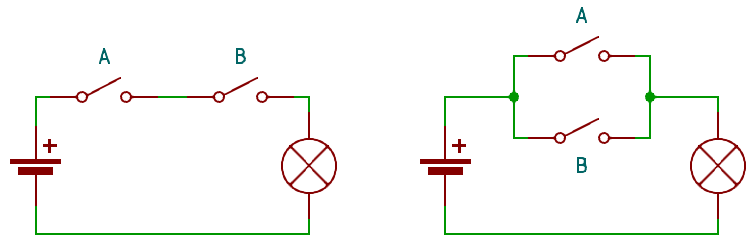
\includegraphics[width=0.7\linewidth,height=\textheight,keepaspectratio]{images/03-logiska-grindar/switch_and_or.png}

\caption{\label{fig-switch-lampa}Logisk analogi: Strömbrytare som
representerar AND- respektive OR-funktion.}

\end{figure}%

Detta exempel med switchar och lampa visar fundamenten i digital
systemdesign:

\begin{itemize}
\tightlist
\item
  \textbf{Ingångar:} Den information vi vill bearbeta.
\item
  \textbf{Logisk funktion:} Den ``regel'' grinden följer (t.ex. ``om A
  och B är sanna\ldots{}'').
\item
  \textbf{Utgång:} Resultatet av operationen.
\end{itemize}

\section{Grinden som abstraktion}\label{grinden-som-abstraktion}

När vi ritar digitala system använder vi oss av en \textbf{abstraktion}.
Vi behöver inte bekymra oss om exakt hur transistorerna inuti en krets
fungerar för att kunna designa en maskin -- vi fokuserar på den logiska
funktionen.

En grind är alltså en ``svart låda'' med förutsägbara egenskaper. Genom
att kombinera dessa enkla grindar kan vi skapa allt från enkla räknare
till extremt komplexa processorer. I kommande avsnitt ska vi lära oss
hur vi systematiskt beskriver vad som händer inuti dessa ``svarta
lådor'' med hjälp av sanningstabeller.

\section{Sanningstabeller: Ett systematiskt
analysverktyg}\label{sanningstabeller-ett-systematiskt-analysverktyg}

För att slippa rita kretsscheman varje gång vi vill förstå en funktion
använder vi \textbf{sanningstabeller}. En sanningstabell är en
matematisk tabell som listar alla tänkbara kombinationer av insignaler
(A och B) och visar vad den resulterande utsignalen (Q) blir för varje
scenario.

Det fina med en sanningstabell är att den är uttömmande. Om vi har \(n\)
stycken insignaler, kommer tabellen alltid att ha \(2^n\) rader. För
våra två grundläggande grindar innebär det \(2^2 = 4\) möjliga
kombinationer.

\subsection{Sanningstabell för
AND-grinden}\label{sanningstabell-fuxf6r-and-grinden}

AND-funktionen (se vänster kretsschema i Figur~\ref{fig-switch-lampa})
kräver att \textbf{båda} insignalerna är 1 för att utsignalen ska bli 1.
Den logiska notationen skrivs ofta som \(A \cdot B = Q\). Notationen är
ett exempel på Booles algebra, som vi kommer till senare.

\begin{longtable}[]{@{}lll@{}}
\caption{Sanningstabell för AND}\label{tbl-and}\tabularnewline
\toprule\noalign{}
A & B & Q (AND) \\
\midrule\noalign{}
\endfirsthead
\toprule\noalign{}
A & B & Q (AND) \\
\midrule\noalign{}
\endhead
\bottomrule\noalign{}
\endlastfoot
0 & 0 & 0 \\
0 & 1 & 0 \\
1 & 0 & 0 \\
1 & 1 & 1 \\
\end{longtable}

\subsection{Sanningstabell för OR-grinden}\label{sec-logiska-grindar}

OR-funktionen (e höger kretsschema i Figur~\ref{fig-switch-lampa})
kräver att \textbf{minst en} av insignalerna är 1 för att utsignalen ska
bli 1. Den logiska notationen skrivs ofta som \(A + B = Q\).

\begin{longtable}[]{@{}lll@{}}
\caption{Sanningstabell för OR}\label{tbl-or}\tabularnewline
\toprule\noalign{}
A & B & Q (OR) \\
\midrule\noalign{}
\endfirsthead
\toprule\noalign{}
A & B & Q (OR) \\
\midrule\noalign{}
\endhead
\bottomrule\noalign{}
\endlastfoot
0 & 0 & 0 \\
0 & 1 & 1 \\
1 & 0 & 1 \\
1 & 1 & 1 \\
\end{longtable}

Att lära sig läsa dessa tabeller är grundbulten i all digital design.
När vi senare börjar kombinera grindar för att bygga mer avancerade
logiska nätverk, använder vi dessa tabeller för att bevisa att våra
kretsar faktiskt utför den logik vi förväntar oss.

\begin{tcolorbox}[enhanced jigsaw, arc=.35mm, bottomrule=.15mm, bottomtitle=1mm, breakable, colback=white, colbacktitle=quarto-callout-note-color!10!white, colframe=quarto-callout-note-color-frame, coltitle=black, left=2mm, leftrule=.75mm, opacityback=0, opacitybacktitle=0.6, rightrule=.15mm, title=\textcolor{quarto-callout-note-color}{\faInfo}\hspace{0.5em}{Exempel: Logik i ett ADAS-system för fordon}, titlerule=0mm, toprule=.15mm, toptitle=1mm]

För att förstå hur logiska grindar samverkar i praktiken kan vi studera
ett förenklat säkerhetssystem i en modern bil. Systemet ska aktivera
bromsarna (Q) under tre specifika förhållanden:

\begin{enumerate}
\def\labelenumi{\arabic{enumi}.}
\tightlist
\item
  Föraren bromsar (A)
\item
  Bilens radar indikerar ett hinder (B)
\item
  Bilens kamera indikerar ett hinder (C)
\end{enumerate}

Logiken för systemet är att bromsen ska aktiveras om \textbf{föraren
bromsar} ELLER (om \textbf{både radar OCH kamera} indikerar hinder).
Matematiskt med Booles algebra kan detta uttryckas som
\(Q = A + (B \cdot C)\).

Här ser vi hur de olika indata-kombinationerna påverkar
bromsaktiveringen. Notera hur de fjärde raden visar hur radarn och
kameran tillsammans kan tvinga fram en bromsning även om föraren inte
trycker på bromspedalen.

\begin{longtable}[]{@{}cccc@{}}
\caption{Sanningstabell för
ADAS-bromsning}\label{tbl-adas}\tabularnewline
\toprule\noalign{}
Förare (A) & Radar (B) & Kamera (C) & Broms (Q) \\
\midrule\noalign{}
\endfirsthead
\toprule\noalign{}
Förare (A) & Radar (B) & Kamera (C) & Broms (Q) \\
\midrule\noalign{}
\endhead
\bottomrule\noalign{}
\endlastfoot
0 & 0 & 0 & 0 \\
0 & 0 & 1 & 0 \\
0 & 1 & 0 & 0 \\
0 & 1 & 1 & 1 \\
1 & 0 & 0 & 1 \\
1 & 0 & 1 & 1 \\
1 & 1 & 0 & 1 \\
1 & 1 & 1 & 1 \\
\end{longtable}

Denna tabell tydliggör systemets säkerhetsfilosofi: föraråtgärden
prioriteras (rad 5-8), men vi har också en redundant säkerhetskontroll
där radarn och kameran måste vara eniga för att aktivera automatisk
nödbromsning (rad 4).

\end{tcolorbox}

\section{Logiska grindar: Symboler och
funktion}\label{logiska-grindar-symboler-och-funktion}

Inom digitaltekniken används två huvudstandarder för att rita grindar:
\textbf{IEC} (den rektangulära formen) och \textbf{ANSI/IEEE} (den
karaktäristiska ``bågformen''). Oberoende av vilken standard som används
är den logiska funktionen alltid densamma.

\begin{figure}

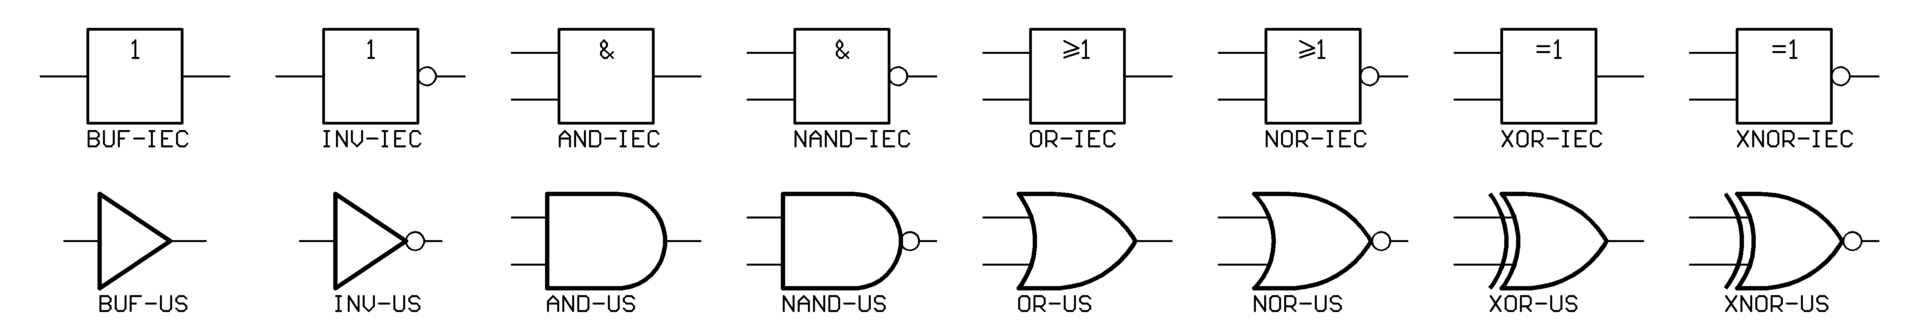
\includegraphics[width=1\linewidth,height=\textheight,keepaspectratio]{images/03-logiska-grindar//Logic-gate-index.png}

\caption{\label{fig-gate-index}Översikt över logiska grindar: Buffer,
NOT (INV = invertering), AND, NAND, OR, NOR, XOR (Exklusivt ELLER) och
XNOR. \protect\newline Källa: Modifierad från
\href{https://de.wikipedia.org/wiki/User:Stefan506}{User:Stefan506} CC
BY-SA 3.0, https://commons.wikimedia.org/w/index.php?curid=460661}

\end{figure}%

Som vi ser i Figur~\ref{fig-gate-index} representerar varje grind en
unik logisk operation. En central princip att notera är
\textbf{inverteringsbubblan} (den lilla cirkeln vid utgången), som i ett
kopplingsschema indikerar en NOT-operation.

Vilka symboler ska man lära sig? Det enkla och jobbiga svaret är både
europeisk och amerikansk standard (ANSI/IEEE). Båda varianterna stöter
man på i olika sorters dokumentation. I denna bok kommer amerikanska
symboler användas, eftersom de finns i datablad för digitaltekniska
kretsar.

\subsection{Buffer och Inverterare
(NOT)}\label{buffer-och-inverterare-not}

En \textbf{Buffer} kopierar insignalen direkt till utgången (\(Q = A\)).
En \textbf{NOT-grind} (inverterare) vänder på signalen så att 1 blir 0
och 0 blir 1 (notationn för NOT är ett rakt streck ovanför variabeln,
\(Q = \overline{A}\)).

\begin{longtable}[]{@{}ccc@{}}
\caption{Sanningstabell för Buffer och
NOT}\label{tbl-buffer-not}\tabularnewline
\toprule\noalign{}
A & Buffer (Q) & NOT (Q) \\
\midrule\noalign{}
\endfirsthead
\toprule\noalign{}
A & Buffer (Q) & NOT (Q) \\
\midrule\noalign{}
\endhead
\bottomrule\noalign{}
\endlastfoot
0 & 0 & 1 \\
1 & 1 & 0 \\
\end{longtable}

\subsection{AND och NAND}\label{and-och-nand}

\textbf{AND-grinden} ger endast 1 om \emph{alla} insignaler är 1.
\textbf{NAND-grinden} (NOT-AND) är dess raka motsats -- den ger 0 endast
om alla insignaler är 1.

\begin{longtable}[]{@{}cccc@{}}
\caption{Sanningstabell för AND och
NAND}\label{tbl-and-nand}\tabularnewline
\toprule\noalign{}
A & B & AND (Q) & NAND (Q) \\
\midrule\noalign{}
\endfirsthead
\toprule\noalign{}
A & B & AND (Q) & NAND (Q) \\
\midrule\noalign{}
\endhead
\bottomrule\noalign{}
\endlastfoot
0 & 0 & 0 & 1 \\
0 & 1 & 0 & 1 \\
1 & 0 & 0 & 1 \\
1 & 1 & 1 & 0 \\
\end{longtable}

\subsection{OR och NOR}\label{or-och-nor}

\textbf{OR-grinden} ger 1 om \emph{minst en} insignal är 1.
\textbf{NOR-grinden} (NOT-OR) ger 1 endast när båda insignalerna är 0.

\begin{longtable}[]{@{}cccc@{}}
\caption{Sanningstabell för OR och NOR}\label{tbl-or-nor}\tabularnewline
\toprule\noalign{}
A & B & OR (Q) & NOR (Q) \\
\midrule\noalign{}
\endfirsthead
\toprule\noalign{}
A & B & OR (Q) & NOR (Q) \\
\midrule\noalign{}
\endhead
\bottomrule\noalign{}
\endlastfoot
0 & 0 & 0 & 1 \\
0 & 1 & 1 & 0 \\
1 & 0 & 1 & 0 \\
1 & 1 & 1 & 0 \\
\end{longtable}

\begin{tcolorbox}[enhanced jigsaw, arc=.35mm, bottomrule=.15mm, bottomtitle=1mm, breakable, colback=white, colbacktitle=quarto-callout-tip-color!10!white, colframe=quarto-callout-tip-color-frame, coltitle=black, left=2mm, leftrule=.75mm, opacityback=0, opacitybacktitle=0.6, rightrule=.15mm, title=\textcolor{quarto-callout-tip-color}{\faLightbulb}\hspace{0.5em}{NOR-grinden och NAND-grinden: De universella byggstenenarna}, titlerule=0mm, toprule=.15mm, toptitle=1mm]

NOR-grinden är tillsammans med NAND-grinden unika eftersom man genom att
kombinera enbart NOR-grindar alternativt bara NAND-grindar kan bygga
\emph{alla} andra logiska funktioner. Detta gör dessa grindar viktiga i
praktisk chip-design. För den som designar hårdvara med logiska grindar
kan det också ha betydelse. IC-kretsar med logiska grindar innehåller
generellt flera stycken grindar av samma typ. Det innebär att man som
hårdvarudesigner ofta har grindar över, som kan avnändas för att
realisera någon annan form av grind. Ett enkelt exempel är att en
NOT-grind enkelt kan byggas med en NOR eller NAND genom att ingångarna
kopplas samman.

\end{tcolorbox}

\subsection{XOR och XNOR}\label{xor-och-xnor}

\textbf{XOR (Exklusivt ELLER)} ger 1 när insignalerna är \emph{olika}.
\textbf{XNOR} (NOT-XOR) ger 1 när insignalerna är \emph{lika}.

\begin{longtable}[]{@{}cccc@{}}
\caption{Sanningstabell för XOR och
XNOR}\label{tbl-xor-xnor}\tabularnewline
\toprule\noalign{}
A & B & XOR (Q) & XNOR (Q) \\
\midrule\noalign{}
\endfirsthead
\toprule\noalign{}
A & B & XOR (Q) & XNOR (Q) \\
\midrule\noalign{}
\endhead
\bottomrule\noalign{}
\endlastfoot
0 & 0 & 0 & 1 \\
0 & 1 & 1 & 0 \\
1 & 0 & 1 & 0 \\
1 & 1 & 0 & 1 \\
\end{longtable}

Notationen för NOR är \(Q = A \oplus B\). XNOR skrivs med hjälp av
invertering som \(Q = \overline{A \oplus B}\) eller med ett annat tecken
\(Q = A \odot B\). I denna bok används notationen
\(Q = \overline{A \oplus B}\).

\subsection{När vi har fler än två
ingångar}\label{nuxe4r-vi-har-fler-uxe4n-tvuxe5-inguxe5ngar}

För de flesta grindar (som AND och OR) är utökningen till fler ingångar
intuitiv. En AND-grind med exempelvis fyra ingångar ger 1 endast om
\emph{alla} fyra är 1. För en OR-grind med med flera ingångar gäller
fortfarande att det räcker att en ingång är 1 för att utgången ska bli
1. Men för XOR-grinden kräver definitionen lite extra eftertanke.

\begin{tcolorbox}[enhanced jigsaw, arc=.35mm, bottomrule=.15mm, bottomtitle=1mm, breakable, colback=white, colbacktitle=quarto-callout-important-color!10!white, colframe=quarto-callout-important-color-frame, coltitle=black, left=2mm, leftrule=.75mm, opacityback=0, opacitybacktitle=0.6, rightrule=.15mm, title=\textcolor{quarto-callout-important-color}{\faExclamation}\hspace{0.5em}{XOR och XNOR med fler än två ingångar}, titlerule=0mm, toprule=.15mm, toptitle=1mm]

Det är lätt att tro att en XOR-grind med tre ingångar ger 1 om
\emph{exakt en} ingång är 1. Den korrekta definitionen är dock att
XOR-grinden fungerar som en \textbf{udda-funktion} (odd parity):

\begin{itemize}
\tightlist
\item
  Utgången är 1 om ett \textbf{udda antal} ingångar är 1.
\item
  Utgången är 0 om ett \textbf{jämnt antal} ingångar är 1.
\end{itemize}

Detta innebär att \(A \oplus B \oplus C\) blir 1 om antingen en eller
alla tre ingångar är 1.

\end{tcolorbox}

För XNOR-grinden är logiken den omvända: den fungerar som en
\textbf{jämn-funktion} (even parity) och ger 1 om ett jämnt antal
ingångar är 1 (inklusive noll ingångar).

\begin{tcolorbox}[enhanced jigsaw, arc=.35mm, bottomrule=.15mm, bottomtitle=1mm, breakable, colback=white, colbacktitle=quarto-callout-note-color!10!white, colframe=quarto-callout-note-color-frame, coltitle=black, left=2mm, leftrule=.75mm, opacityback=0, opacitybacktitle=0.6, rightrule=.15mm, title=\textcolor{quarto-callout-note-color}{\faInfo}\hspace{0.5em}{Exempel: Analys av 3-ingångars XOR}, titlerule=0mm, toprule=.15mm, toptitle=1mm]

\begin{longtable}[]{@{}cccc@{}}
\caption{Sanningstabell för 3-ingångars
XOR}\label{tbl-xor-3-in}\tabularnewline
\toprule\noalign{}
A & B & C & Q (XOR) \\
\midrule\noalign{}
\endfirsthead
\toprule\noalign{}
A & B & C & Q (XOR) \\
\midrule\noalign{}
\endhead
\bottomrule\noalign{}
\endlastfoot
0 & 0 & 0 & 0 \\
0 & 0 & 1 & 1 \\
0 & 1 & 0 & 1 \\
0 & 1 & 1 & 0 \\
1 & 0 & 0 & 1 \\
1 & 0 & 1 & 0 \\
1 & 1 & 0 & 0 \\
1 & 1 & 1 & 1 \\
\end{longtable}

När vi utökar XOR-grinden till tre ingångar (\(A \oplus B \oplus C\))
lämnar vi den enkla ``en-av-tre''-logiken bakom oss. Istället ser vi att
utsignalen \(Q\) blir 1 endast när antalet ettor på ingångarna är udda.
Som tabellen i Tabell~\ref{tbl-xor-3-in} visar, får vi en hög utsignal
(\(Q=1\)) i följande fall: * Precis en ingång är 1 (rad 2, 3, 5). * Alla
tre ingångarna är 1 (rad 8).

Detta bekräftar definitionen av XOR som en ``udda-funktion''. Om vi
skulle addera en fjärde ingång (\(D\)) skulle utsignalen bli 1 igen om
totalt antal ettor är udda (1 eller 3 stycken).

\end{tcolorbox}

\subsection{Från teori till hårdvara:
7400-serien}\label{fruxe5n-teori-till-huxe5rdvara-7400-serien}

För att bygga digital elektronik för enklare applikationer i
verkligheten använder vi integrerade kretsar. Den mest klassiska
familjen är \textbf{7400-serien}, där kapslar ofta innehåller
``Quad''-logik, det vill säga fyra grindar i samma hus. Dessa klassiska
kretsar användes förr i stor skala för att bygga upp komplexa digitala
lösningar. Idag så byggs mer komplex digitalelektronik primärt med
\textbf{FPGA} (field-programmable gate array) eller \textbf{ASIC}
(application-specific integrated circuit), där logiken beskrivs med
hårdvarubeskrivande språk som VHDL eller Verilog. Men 7400-serien är
fortfarande mycket användbar inom exempelvis embeddedområdet när man
behöver skapa enklare digitala funktioner.

Det är dock viktigt att förstå att 7400-serien omfattar massor av olika
kretsar, inte bara grindar. Några exempel är: * \textbf{Flip-flops och
register:} För att lagra binär information. * \textbf{Räknare:} För att
skapa klockade sekvenser. * \textbf{Multiplexer:} För att välja mellan
olika insignaler.

\begin{longtable}[]{@{}lll@{}}
\caption{Klassiska grind-kretsar i
7400-serien}\label{tbl-7400-gates}\tabularnewline
\toprule\noalign{}
Krets & Funktion & Antal grindar \\
\midrule\noalign{}
\endfirsthead
\toprule\noalign{}
Krets & Funktion & Antal grindar \\
\midrule\noalign{}
\endhead
\bottomrule\noalign{}
\endlastfoot
\textbf{7400} & NAND-grindar (2-ingångar) & 4 \\
\textbf{7402} & NOR-grindar (2-ingångar) & 4 \\
\textbf{7404} & Inverterare (NOT) & 6 \\
\textbf{7408} & AND-grindar (2-ingångar) & 4 \\
\textbf{7432} & OR-grindar (2-ingångar) & 4 \\
\textbf{7486} & XOR-grindar (2-ingångar) & 4 \\
\textbf{74266} & XNOR-grindar (2-ingångar) & 4 \\
\end{longtable}

\begin{tcolorbox}[enhanced jigsaw, arc=.35mm, bottomrule=.15mm, bottomtitle=1mm, breakable, colback=white, colbacktitle=quarto-callout-note-color!10!white, colframe=quarto-callout-note-color-frame, coltitle=black, left=2mm, leftrule=.75mm, opacityback=0, opacitybacktitle=0.6, rightrule=.15mm, title=\textcolor{quarto-callout-note-color}{\faInfo}\hspace{0.5em}{Exempel: Realisering av ADAS-system}, titlerule=0mm, toprule=.15mm, toptitle=1mm]

För att realisera vårt exempel med ADAS-system från
Avsnitt~\ref{sec-logiska-grindar} i hårdvara använder vi oss av två
olika 14-pinnars kretsar ur 7400-serien. Detta är ett utmärkt exempel på
hur vi kombinerar olika ``Quad-logik''-kretsar för att skapa en
funktionell enhet. ADAS-systemet kunde skrivas som
(\(Q = A + (B \cdot C)\)), dvs. en AND-funktion som kombinerar två
ingångar (radar B och kamera C) som går vidare till en OR-funktion som
kombinerar AND-grindens utgång med ytterligare en ingång (föraren A).

\textbf{Komponentval}

\begin{itemize}
\tightlist
\item
  \textbf{7408 (Quad 2-input AND):} Vi använder en av de fyra grindarna
  för att kombinera \textbf{Radar (B)} och \textbf{Kamera (C)}.
\item
  \textbf{7432 (Quad 2-input OR):} Vi använder en av de fyra grindarna
  för att summera AND-grindens utgång med \textbf{Förarens input (A)}.
\end{itemize}

\textbf{Kopplingsbeskrivning}

\begin{enumerate}
\def\labelenumi{\arabic{enumi}.}
\tightlist
\item
  \textbf{Radar (B)} och \textbf{Kamera (C)} ansluts till ingångarna på
  en grind i 7408-kretsen (t.ex. pin 1 och 2).
\item
  Utgången från denna AND-grind (t.ex. pin 3) kopplas till en av
  ingångarna på en grind i 7432-kretsen (t.ex. pin 1).
\item
  \textbf{Föraren (A)} kopplas till den andra ingången på samma OR-grind
  i 7432-kretsen (pin 2).
\item
  Utgången på OR-grinden (pin 3 på 7432) ger oss den slutgiltiga
  \textbf{Bromssignalen (Q)}.
\end{enumerate}

\begin{figure}[H]

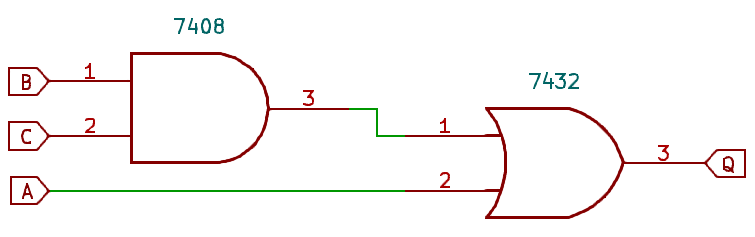
\includegraphics[width=0.5\linewidth,height=\textheight,keepaspectratio]{images/03-logiska-grindar/ADAS_realization.png}

\caption{\label{fig-ADAS}Kretsschema för logiska funktionen för ett
ADAS-system.}

\end{figure}%

\begin{longtable}[]{@{}lll@{}}
\caption{Kopplingsöversikt för
ADAS-system}\label{tbl-adas-wiring}\tabularnewline
\toprule\noalign{}
Signaler & Komponent & Pin (Exempel) \\
\midrule\noalign{}
\endfirsthead
\toprule\noalign{}
Signaler & Komponent & Pin (Exempel) \\
\midrule\noalign{}
\endhead
\bottomrule\noalign{}
\endlastfoot
B \& C (Radar/Kamera) & 7408 (AND) & 1, 2 (In) / 3 (Ut) \\
A (Förare) \& Utgång 7408 & 7432 (OR) & 1, 2 (In) / 3 (Ut) \\
Bromssignal (Q) & - & 3 (Ut) \\
\end{longtable}

\end{tcolorbox}

\begin{tcolorbox}[enhanced jigsaw, arc=.35mm, bottomrule=.15mm, bottomtitle=1mm, breakable, colback=white, colbacktitle=quarto-callout-important-color!10!white, colframe=quarto-callout-important-color-frame, coltitle=black, left=2mm, leftrule=.75mm, opacityback=0, opacitybacktitle=0.6, rightrule=.15mm, title=\textcolor{quarto-callout-important-color}{\faExclamation}\hspace{0.5em}{Hantering av oanvända grindar}, titlerule=0mm, toprule=.15mm, toptitle=1mm]

Eftersom 7408 och 7432 i exemplet ovan båda är ``Quad''-kretsar har vi
tre grindar över i varje kapsel som inte används. Kom ihåg att
\textbf{oanvända ingångar aldrig får lämnas flytande (oanslutna)}. En
flytande ingång fungerar som en antenn för elektriskt brus. Koppla dessa
ingångar till antingen jord (\(0\text{V}\)) eller matningsspänning
(\(+5\text{V}\)) för att undvika att kretsen börjar bete sig konstigt.

\end{tcolorbox}

\bookmarksetup{startatroot}

\chapter{Boolesk algebra -- Logikens
matematik}\label{boolesk-algebra-logikens-matematik}

\definecolor{highlight_249_115_022}{rgb}{0.976, 0.451, 0.086}
\definecolor{highlight_124_058_237}{rgb}{0.486, 0.227, 0.929}
\definecolor{highlight_016_185_129}{rgb}{0.063, 0.725, 0.506}
\definecolor{highlight_239_068_068}{rgb}{0.937, 0.267, 0.267}
\definecolor{highlight_059_130_246}{rgb}{0.231, 0.510, 0.965}
\definecolor{highlight_245_158_011}{rgb}{0.961, 0.620, 0.043}

\section{Varför räkna på logik?}\label{varfuxf6r-ruxe4kna-puxe5-logik}

När vi arbetar med digitalteknik är det lätt att tro att det räcker med
``sunt förnuft''. Om en lampa ska lysa när två knappar trycks in, drar
vi slutsatsen att vi behöver en AND-grind. Men i verkliga system, där
dussintals sensorer och signaler samverkar, räcker intuitionen inte
till. Här kommer \textbf{Boolesk algebra} in i bilden. Det är ett
matematiskt system, utvecklat av George Boole på 1800-talet, som låter
oss beskriva logiska samband med variabler och operatorer istället för
bara ord eller krångliga scheman.

Du kanske frågar dig: \emph{``Varför måste jag lära mig formler när jag
kan tänka ut lösningen?''} Svaret är enkelt: \textbf{Optimering.} En
duktig ingenjör nöjer sig inte med en krets som bara ``fungerar''. Vi
vill bygga kretsar som är:

\begin{itemize}
\tightlist
\item
  \textbf{Billigare:} Färre grindar innebär lägre komponentkostnader.
\item
  \textbf{Mindre:} Mindre yta på kretskortet ger mer kompakta produkter.
\item
  \textbf{Snabbare:} Varje grind signalen passerar skapar en liten
  fördröjning. Färre steg ger snabbare system.
\item
  \textbf{Strömsnåla:} Varje transistor som switchar drar energi.
\end{itemize}

Genom att använda de Booleska lagarna kan vi ta ett komplext uttryck --
som vid första anblick ser ut att kräva fem olika kretsar -- och bevisa
att det i själva verket kan ersättas av en enda ledare eller en enkel
grind. Algebran ger oss ett universellt språk att dokumentera våra
lösningar med, så att kollegor kan följa vårt resonemang svart på vitt.

\section{Den logiska syntaxen}\label{den-logiska-syntaxen}

För att kunna räkna med logik behöver vi ett gemensamt språk. Inom
digitaltekniken använder vi standardiserad notation för att beskriva
grindar och deras funktioner i formler. När vi skriver Booleska uttryck
använder vi tre huvudoperationer, NOT, AND och OR. Notera att det finns
flera olika sätt att skriva samma sak beroende på vilken litteratur man
läser:

\begin{longtable}[]{@{}llll@{}}
\caption{Logiska operationer och notation. Tabellen visar
standardnotation och alternativa sätt att uttrycka Booleska funktioner.
Invertering, logisk produkt och logisk summa räknas som axiom, vilket
kan sägas vara grundantaganden som hålls för sanna och utgör basen för
det teoretiska ramverket.}\label{tbl-booleska_notationer}\tabularnewline
\toprule\noalign{}
Funktion & Beskrivning & Notation (Standard) & Alternativ notation \\
\midrule\noalign{}
\endfirsthead
\toprule\noalign{}
Funktion & Beskrivning & Notation (Standard) & Alternativ notation \\
\midrule\noalign{}
\endhead
\bottomrule\noalign{}
\endlastfoot
\textbf{NOT} & Invertering & \(\overline{A}\) & \(A'\) eller
\(NOT(A)\) \\
\textbf{AND} & Logisk produkt & \(A \cdot B\) & \(AB\) \\
\textbf{OR} & Logisk summa & \(A + B\) & \(A \lor B\) \\
\textbf{XOR} & Exklusivt ELLER & \(A \oplus B\) &
\(A \text{ EOR } B\) \\
\textbf{NAND} & Inverterad AND & \(\overline{A \cdot B}\) &
\(A \uparrow B\) \\
\textbf{NOR} & Inverterad OR & \(\overline{A + B}\) &
\(A \downarrow B\) \\
\textbf{XNOR} & Inverterad XOR & \(\overline{A \oplus B}\) &
\(A \odot B\) \\
\end{longtable}

I denna litteratur används standardnotationen.

För att tolka notationen på ett korrekt sätt behövs vissa räkneregler
som vi till stor känner igen från den vanliga algebran.

\begin{itemize}
\tightlist
\item
  \textbf{Prioritetsordning:} Precis som i vanlig matematik
  (\(1 + 2 \cdot 3\)) finns en prioriteringsordning. \textbf{NOT}
  (invertering) utförs alltid först, följt av \textbf{AND}
  (multiplikation), och sist \textbf{OR} (addition).
\item
  \textbf{Parenteser:} Om du vill styra ordningen, använd parenteser
  precis som i vanlig algebra. Exempel: \((A + B) \cdot C\) innebär att
  OR-operationen sker före AND.
\end{itemize}

\begin{tcolorbox}[enhanced jigsaw, arc=.35mm, bottomrule=.15mm, bottomtitle=1mm, breakable, colback=white, colbacktitle=quarto-callout-tip-color!10!white, colframe=quarto-callout-tip-color-frame, coltitle=black, left=2mm, leftrule=.75mm, opacityback=0, opacitybacktitle=0.6, rightrule=.15mm, title=\textcolor{quarto-callout-tip-color}{\faLightbulb}\hspace{0.5em}{Visuell översikt}, titlerule=0mm, toprule=.15mm, toptitle=1mm]

Det är viktigt att snabbt kunna koppla ihop en matematisk symbol med en
fysisk grind. \textbf{Kom ihåg:}

\begin{itemize}
\tightlist
\item
  När du ser \(A \cdot B\) (AND), tänk på det som \textbf{``både A och B
  måste vara 1''}.
\item
  När du ser \(A + B\) (OR), tänk på det som \textbf{``antingen A eller
  B (eller båda) måste vara 1''}.
\end{itemize}

\end{tcolorbox}

\section{Från sanningstabell till
uttryck}\label{fruxe5n-sanningstabell-till-uttryck}

Innan vi kan börja förenkla måste vi kunna översätta en
funktionsbeskrivning till matematik. Vi gör detta genom att titta på en
sanningstabell och extrahera de rader där något faktiskt händer. Precis
som att binära tal har två symboler, kan detta göras på två olika sätt
genom att fokusera på 0 eller 1.

\subsection{Mintermer: Fokus på när det händer
(1:or)}\label{sec-mintermer}

Det vanligaste sättet är att skapa en \textbf{summa av produkter}. Vi
tittar på varje rad i sanningstabellen där utgången \(Y = 1\).

Varje sådan rad bildar en \textbf{minterm}, där vi multiplicerar (AND)
ihop de insignaler som krävs:

\begin{itemize}
\tightlist
\item
  Om en insignal är \textbf{0} på raden, skriver vi den som inverterad
  (\(\overline{A}\)).
\item
  Om en insignal är \textbf{1} på raden, skriver vi den som den är
  (\(A\)).
\end{itemize}

\begin{tcolorbox}[enhanced jigsaw, arc=.35mm, bottomrule=.15mm, bottomtitle=1mm, breakable, colback=white, colbacktitle=quarto-callout-note-color!10!white, colframe=quarto-callout-note-color-frame, coltitle=black, left=2mm, leftrule=.75mm, opacityback=0, opacitybacktitle=0.6, rightrule=.15mm, title=\textcolor{quarto-callout-note-color}{\faInfo}\hspace{0.5em}{Enkel larmkrets}, titlerule=0mm, toprule=.15mm, toptitle=1mm]

Vi vill att ett larm (\(Y\)) ska gå om sensor \(A\) är aktiverad (1)
samtidigt som sensor \(B\) är inaktiv (0).

\begin{longtable}[]{@{}cccl@{}}
\caption{Sanningstabell för enkel larmkrets med två
ingångar.}\label{tbl-tt-alarm}\tabularnewline
\toprule\noalign{}
A & B & Y & Minterm \\
\midrule\noalign{}
\endfirsthead
\toprule\noalign{}
A & B & Y & Minterm \\
\midrule\noalign{}
\endhead
\bottomrule\noalign{}
\endlastfoot
0 & 0 & 0 & - \\
0 & 1 & 0 & - \\
1 & 0 & \textbf{1} & \(A \cdot \overline{B}\) \\
1 & 1 & 0 & - \\
\end{longtable}

Detta ger oss det matematiska uttrycket \(Y = A \cdot \overline{B}\).
Med detta som grund kan vi börja använda logikens lagar för att
manipulera och förenkla betydligt mer komplexa system.

\end{tcolorbox}

\begin{tcolorbox}[enhanced jigsaw, arc=.35mm, bottomrule=.15mm, bottomtitle=1mm, breakable, colback=white, colbacktitle=quarto-callout-note-color!10!white, colframe=quarto-callout-note-color-frame, coltitle=black, left=2mm, leftrule=.75mm, opacityback=0, opacitybacktitle=0.6, rightrule=.15mm, title=\textcolor{quarto-callout-note-color}{\faInfo}\hspace{0.5em}{Exempel: Säkerhetsspärr med tre insignaler}, titlerule=0mm, toprule=.15mm, toptitle=1mm]

Vi har tre sensorer till en maskin: \textbf{Startknapp (\(A\))},
\textbf{Säkerhetslucka (\(B\))} och \textbf{Serviceläge (\(C\))}.
Maskinen ska starta (\(Y=1\)) i två specifika fall. Dels när vanliga
operatören kör maskinen och har stängt säkerhetsluckan och tryckt på
startknappen. Men den ska också kunna köras av servicetekniker med öppen
lucka när startknappen inte är aktiverad. Vi ställer upp
sanningstabellen för att identifiera våra mintermer.

\begin{longtable}[]{@{}ccccl@{}}
\caption{Sanningstabell för säkerhetsspärr med tre
ingångar.}\label{tbl-tt-safety-circuit}\tabularnewline
\toprule\noalign{}
A & B & C & Y & Minterm \\
\midrule\noalign{}
\endfirsthead
\toprule\noalign{}
A & B & C & Y & Minterm \\
\midrule\noalign{}
\endhead
\bottomrule\noalign{}
\endlastfoot
0 & 0 & 0 & 0 & - \\
0 & 0 & 1 & \textbf{1} & \(\overline{A} \cdot \overline{B} \cdot C\) \\
0 & 1 & 0 & 0 & - \\
0 & 1 & 1 & 0 & - \\
1 & 0 & 0 & 0 & - \\
1 & 0 & 1 & 0 & - \\
1 & 1 & 0 & \textbf{1} & \(A \cdot B \cdot \overline{C}\) \\
1 & 1 & 1 & 0 & - \\
\end{longtable}

För att gå från tabell till uttryck identifieras de rader där utgängen
är 1. Det blir två produkttermer,
\(\overline{A} \cdot \overline{B} \cdot C\) \textbar{} respektive
\(A \cdot B \cdot \overline{C}\) \textbar. Dessa summeras till ett
totalt uttryck (eller kopplas samman i en OR-grind om vi tänker
realisering). Vi skapar alltså summan (OR) av de två mintermerna där
\(Y=1\):
\[Y = (\overline{A} \cdot \overline{B} \cdot C) + (A \cdot B \cdot \overline{C})\]

\end{tcolorbox}

\begin{tcolorbox}[enhanced jigsaw, arc=.35mm, bottomrule=.15mm, bottomtitle=1mm, breakable, colback=white, colbacktitle=quarto-callout-tip-color!10!white, colframe=quarto-callout-tip-color-frame, coltitle=black, left=2mm, leftrule=.75mm, opacityback=0, opacitybacktitle=0.6, rightrule=.15mm, title=\textcolor{quarto-callout-tip-color}{\faLightbulb}\hspace{0.5em}{Så här läser du uttrycket}, titlerule=0mm, toprule=.15mm, toptitle=1mm]

När du ser uttrycket
\(Y = (\overline{A} \cdot \overline{B} \cdot C) + (A \cdot B \cdot \overline{C})\)
kan du läsa det som: \emph{``Maskinen startar om (A är 0 OCH B är 0 OCH
C är 1) ELLER om (A är 1 OCH B är 1 OCH C är 0).''} Parenteserna hjälper
oss att se de två separata logiska vägarna tydligt.

\end{tcolorbox}

\subsection{Maxtermer: Fokus på när det inte händer
(0:or)}\label{maxtermer-fokus-puxe5-nuxe4r-det-inte-huxe4nder-0or}

Ibland är det enklare eller mer effektivt att beskriva när en utgång
\textbf{inte} ska vara aktiv. Detta gör vi genom att titta på de rader
där utgången \(Y = 0\). Vi skapar då en \textbf{produkt av summor}.

Varje rad där \(Y = 0\) bildar en \textbf{maxterm}, där vi adderar (OR)
insignalerna: * Om en insignal är \textbf{1} på raden, skriver vi den
som inverterad (\(\overline{A}\)). * Om en insignal är \textbf{0} på
raden, skriver vi den som den är (\(A\)).

Låt oss använda samma larmkrets som tidigare, men nu extraherar vi de
rader där \(Y = 0\).

\begin{tcolorbox}[enhanced jigsaw, arc=.35mm, bottomrule=.15mm, bottomtitle=1mm, breakable, colback=white, colbacktitle=quarto-callout-note-color!10!white, colframe=quarto-callout-note-color-frame, coltitle=black, left=2mm, leftrule=.75mm, opacityback=0, opacitybacktitle=0.6, rightrule=.15mm, title=\textcolor{quarto-callout-note-color}{\faInfo}\hspace{0.5em}{Exempel: Maxtermer för larmkretsen}, titlerule=0mm, toprule=.15mm, toptitle=1mm]

\begin{longtable}[]{@{}cccc@{}}
\caption{Samma sanningstabell som Tabell~\ref{tbl-tt-alarm}, men med
maxtermer i stället för
mintermer.}\label{tbl-tt-alarm-maxterms}\tabularnewline
\toprule\noalign{}
A & B & Y & Maxterm (A+B) \\
\midrule\noalign{}
\endfirsthead
\toprule\noalign{}
A & B & Y & Maxterm (A+B) \\
\midrule\noalign{}
\endhead
\bottomrule\noalign{}
\endlastfoot
0 & 0 & \textbf{0} & \((A + B)\) \\
0 & 1 & \textbf{0} & \((A + \overline{B})\) \\
1 & 0 & 1 & - \\
1 & 1 & \textbf{0} & \((\overline{A} + \overline{B})\) \\
\end{longtable}

För att få det färdiga uttrycket multiplicerar (AND) vi ihop dessa
maxtermer:
\(Y = (A + B) \cdot (A + \overline{B}) \cdot (\overline{A} + \overline{B})\)
En notering är att detta ser mycket mer komplicerat ut än när samma
exempel bearbetades i Avsnitt~\ref{sec-mintermer}. Det stämmer mycket
riktigt, men man kan välja en av dessa två metoder för att bygga upp
sitt booleska uttryck.
\(Y = (A + B) \cdot (A + \overline{B}) \cdot (\overline{A} + \overline{B})\)
är alltså ekvivalent med \(A \cdot \overline{B}\).

\end{tcolorbox}

Vilken metod ska man välja? Detta kan kännas som ``tårta på tårta'' --
varför ha två metoder? Svaret är \textbf{minimering} och skapa så enkla
förutsättningar som möjligt innan förenkling och optimering sker.

\begin{itemize}
\tightlist
\item
  \textbf{Mintermer (Sum of Products):} Används ofta när det finns få
  rader med 1:or i sanningstabellen.
\item
  \textbf{Maxtermer (Product of Sums):} Används ofta när det finns få
  rader med 0:or i sanningstabellen.
\end{itemize}

\begin{tcolorbox}[enhanced jigsaw, arc=.35mm, bottomrule=.15mm, bottomtitle=1mm, breakable, colback=white, colbacktitle=quarto-callout-tip-color!10!white, colframe=quarto-callout-tip-color-frame, coltitle=black, left=2mm, leftrule=.75mm, opacityback=0, opacitybacktitle=0.6, rightrule=.15mm, title=\textcolor{quarto-callout-tip-color}{\faLightbulb}\hspace{0.5em}{Tips från ingenjören:}, titlerule=0mm, toprule=.15mm, toptitle=1mm]

I praktiken kommer du oftast att använda mintermer för att ställa upp
din första ``råa'' logik. När du väl har uttrycket på plats använder du
Boolesk algebra (som vi går igenom i nästa avsnitt) för att förenkla
uttrycket till minsta möjliga antal grindar, oavsett vilken metod du
startade med.

\end{tcolorbox}

\section{Grundläggande Booleska
lagar}\label{grundluxe4ggande-booleska-lagar}

När vi har översatt ett logiskt problem till ett matematiskt uttryck får
vi ofta en lösning som är komplex och kräver onödigt många grindar. För
att bygga en effektiv krets använder vi Boolesk algebra för att förenkla
uttrycket. Här är de grundläggande verktygen vi använder för att
manipulera våra uttryck.

\begin{longtable}[]{@{}
  >{\raggedright\arraybackslash}p{(\linewidth - 4\tabcolsep) * \real{0.3333}}
  >{\raggedright\arraybackslash}p{(\linewidth - 4\tabcolsep) * \real{0.3333}}
  >{\raggedright\arraybackslash}p{(\linewidth - 4\tabcolsep) * \real{0.3333}}@{}}
\caption{Grundläggande Booleska
lagar.}\label{tbl-booleska_grundlagar}\tabularnewline
\toprule\noalign{}
\begin{minipage}[b]{\linewidth}\raggedright
Lag
\end{minipage} & \begin{minipage}[b]{\linewidth}\raggedright
AND-form
\end{minipage} & \begin{minipage}[b]{\linewidth}\raggedright
OR-form
\end{minipage} \\
\midrule\noalign{}
\endfirsthead
\toprule\noalign{}
\begin{minipage}[b]{\linewidth}\raggedright
Lag
\end{minipage} & \begin{minipage}[b]{\linewidth}\raggedright
AND-form
\end{minipage} & \begin{minipage}[b]{\linewidth}\raggedright
OR-form
\end{minipage} \\
\midrule\noalign{}
\endhead
\bottomrule\noalign{}
\endlastfoot
\textbf{Identitet} & \(A \cdot 1 = A\) & \(A + 0 = A\) \\
\textbf{Noll- och ett-lag} & \(A \cdot 0 = 0\) & \(A + 1 = 1\) \\
\textbf{Idempotens} & \(A \cdot A = A\) & \(A + A = A\) \\
\textbf{Invertering} & \(A \cdot \overline{A} = 0\) &
\(A + \overline{A} = 1\) \\
\textbf{Dubbel negation} & \(\overline{\overline{A}} = A\) & - \\
\end{longtable}

Utöver dessa lagar i Tabell~\ref{tbl-booleska_grundlagar} finns de
\textbf{kommutativa}, \textbf{associativa} och \textbf{distributiva}
lagarna (algebraiska lagar), som fungerar precis som i vanlig matematik
(se Tabell~\ref{tbl-booleska_algebraiska_lagar}).

\begin{longtable}[]{@{}
  >{\raggedright\arraybackslash}p{(\linewidth - 4\tabcolsep) * \real{0.3333}}
  >{\raggedright\arraybackslash}p{(\linewidth - 4\tabcolsep) * \real{0.3333}}
  >{\raggedright\arraybackslash}p{(\linewidth - 4\tabcolsep) * \real{0.3333}}@{}}
\caption{Algebraiska Booleska
lagar.}\label{tbl-booleska_algebraiska_lagar}\tabularnewline
\toprule\noalign{}
\begin{minipage}[b]{\linewidth}\raggedright
Lag
\end{minipage} & \begin{minipage}[b]{\linewidth}\raggedright
AND-form
\end{minipage} & \begin{minipage}[b]{\linewidth}\raggedright
OR-form
\end{minipage} \\
\midrule\noalign{}
\endfirsthead
\toprule\noalign{}
\begin{minipage}[b]{\linewidth}\raggedright
Lag
\end{minipage} & \begin{minipage}[b]{\linewidth}\raggedright
AND-form
\end{minipage} & \begin{minipage}[b]{\linewidth}\raggedright
OR-form
\end{minipage} \\
\midrule\noalign{}
\endhead
\bottomrule\noalign{}
\endlastfoot
\textbf{Kommutativ} & \(A \cdot B = B \cdot A\) & \(A + B = B + A\) \\
\textbf{Associativ} & \(A \cdot (B \cdot C) = (A \cdot B) \cdot C\) &
\(A + (B + C) = (A + B) + C\) \\
\textbf{Distributiv} & \(A \cdot (B + C) = A \cdot B + A \cdot C\) &
\(A + (B \cdot C) = (A + B) \cdot (A + C)\) \\
\end{longtable}

\section{De Morgans lagar}\label{de-morgans-lagar}

De Morgans lagar är det absolut viktigaste verktyget för att hantera
inverterade uttryck när bearbetning av logiska uttryck sker. Gäller
särskilt när vi arbetar med NAND- och NOR-logik. De beskriver hur en
``NOT''-operation påverkar en AND- respektive OR-grind.

De två lagarna lyder:

\begin{itemize}
\tightlist
\item
  \(\overline{A \cdot B} = \overline{A} + \overline{B}\)
\item
  \(\overline{A + B} = \overline{A} \cdot \overline{B}\)
\end{itemize}

Lagarna är enkla att bevisa genom att ställa upp sanningstabeller för
vänster led respektive höger led.

\begin{tcolorbox}[enhanced jigsaw, arc=.35mm, bottomrule=.15mm, bottomtitle=1mm, breakable, colback=white, colbacktitle=quarto-callout-tip-color!10!white, colframe=quarto-callout-tip-color-frame, coltitle=black, left=2mm, leftrule=.75mm, opacityback=0, opacitybacktitle=0.6, rightrule=.15mm, title=\textcolor{quarto-callout-tip-color}{\faLightbulb}\hspace{0.5em}{Ingenjörens minnesregel: ``Bryt och byt''}, titlerule=0mm, toprule=.15mm, toptitle=1mm]

När du ska förenkla ett uttryck med ett långt överstreck, följ dessa två
steg:

\begin{enumerate}
\def\labelenumi{\arabic{enumi}.}
\tightlist
\item
  \textbf{Bryt:} Dela upp det långa överstrecket i flera kortare över
  varje enskild variabel.
\item
  \textbf{Byt:} Byt ut operationen mellan variablerna -- ändra AND
  (\(\cdot\)) till OR (\(+\)), eller OR (\(+\)) till AND (\(\cdot\)).
\end{enumerate}

\end{tcolorbox}

\begin{tcolorbox}[enhanced jigsaw, arc=.35mm, bottomrule=.15mm, bottomtitle=1mm, breakable, colback=white, colbacktitle=quarto-callout-note-color!10!white, colframe=quarto-callout-note-color-frame, coltitle=black, left=2mm, leftrule=.75mm, opacityback=0, opacitybacktitle=0.6, rightrule=.15mm, title=\textcolor{quarto-callout-note-color}{\faInfo}\hspace{0.5em}{Exempel: Bearbetning av uttryck med hjälp av De Morgan}, titlerule=0mm, toprule=.15mm, toptitle=1mm]

Om vi har uttrycket \(\overline{A + \overline{B}}\), så bryter vi
överstrecket över \(A\) och \(\overline{B}\), och byter samtidigt \(+\)
till \(\cdot\):
\(\overline{A + \overline{B}} = \overline{A} \cdot \overline{\overline{B}} = \overline{A} \cdot B\)

\end{tcolorbox}

\section{Konsensuslagarna}\label{konsensuslagarna}

Konsensuslagarna är användbara då man har ``överlappande'' uttryck och
har en redundant term i sitt Booleska uttryck. De kan vara svåra att
identifiera i uttryck eftersom de finns i uttryck som ser ut att vara
färdigförenklade. De finns i två former:

\begin{itemize}
\tightlist
\item
  \(A \cdot B + \overline{A} \cdot C + B \cdot C = A \cdot B + \overline{A} \cdot C\)
\item
  \((A + B) \cdot (\overline{A} + C) \cdot (B + C) = (A + B) \cdot (\overline{A} + C)\)
\end{itemize}

Lyckligtvis så kommer en metod presenteras i
Avsnitt~\ref{sec-Karnaugh-diagram} där dessa lagar hanteras per
automatik. Då kommer vi introducera Karnaughdiagram, som är en grafisk
lösningsmetod för att förenkla logiska uttryck från sanningstabell.

\section{Algebraisk förenkling -- en
steg-för-steg-metod}\label{algebraisk-fuxf6renkling-en-steg-fuxf6r-steg-metod}

Nu när vi har verktygen (de algebraiska lagarna och De Morgan) är det
dags att använda dem för att faktiskt bygga billigare och snabbare
kretsar. Ett komplext uttryck kräver många grindar, vilket innebär mer
värmeutveckling, högre kostnad och längre signalfördröjning.

När du får ett logiskt uttryck, kan det ofta vara bra att följa denna
``checklista'' för att systematiskt förenkla det:

\begin{enumerate}
\def\labelenumi{\arabic{enumi}.}
\tightlist
\item
  \textbf{Expandera:} Använd den distributiva lagen för att lösa upp
  parenteser.
\item
  \textbf{Identifiera:} Leta efter termer som kan förenklas med
  speciallagarna (t.ex. \(A + \overline{A} = 1\) eller
  \(A \cdot A = A\)).
\item
  \textbf{Bryt ut:} Om möjligt, bryt ut gemensamma variabler för att
  skapa förenklingsbara parenteser.
\item
  \textbf{De Morgan:} Om du har långa överstreck, använd ``Bryt och
  byt'' för att förenkla inverteringar.
\end{enumerate}

Numreringen i checklistan ska inte ses som en ordningsföljd som alltid
ska följas strikt. Ibland så behöver man till exempel börja med De
Morgan innan det går att arbeta vidare med förenkling.

\begin{tcolorbox}[enhanced jigsaw, arc=.35mm, bottomrule=.15mm, bottomtitle=1mm, breakable, colback=white, colbacktitle=quarto-callout-note-color!10!white, colframe=quarto-callout-note-color-frame, coltitle=black, left=2mm, leftrule=.75mm, opacityback=0, opacitybacktitle=0.6, rightrule=.15mm, title=\textcolor{quarto-callout-note-color}{\faInfo}\hspace{0.5em}{Exempel: Förenkling med bryt-ut-metoden}, titlerule=0mm, toprule=.15mm, toptitle=1mm]

Vi vill förenkla uttrycket: \(Y = A \cdot B + A \cdot \overline{B}\)

\begin{enumerate}
\def\labelenumi{\arabic{enumi}.}
\item
  \textbf{Bryt ut:} Vi ser att \(A\) är en gemensam faktor i båda
  termerna. Vi använder den distributiva lagen baklänges för att bryta
  ut \(A\): \(Y = A \cdot (B + \overline{B})\)
\item
  \textbf{Identifiera:} Vi vet från våra räknelagar (Invertering) att
  \(B + \overline{B} = 1\). Vi byter ut parentesen mot en etta:
  \(Y = A \cdot 1\)
\item
  \textbf{Slutresultat:} Enligt identitetslagen är \(A \cdot 1 = A\).
  \(Y = A\)
\end{enumerate}

Hårdvarumässigt är detta stor skillnad! Från en krets som ursprungligen
krävde två AND-grindar, en inverterare och en OR-grind, har vi nu
reducerat det hela till en enkel ledning där utsignalen helt enkelt
följer insignalen A.

\end{tcolorbox}

\begin{tcolorbox}[enhanced jigsaw, arc=.35mm, bottomrule=.15mm, bottomtitle=1mm, breakable, colback=white, colbacktitle=quarto-callout-note-color!10!white, colframe=quarto-callout-note-color-frame, coltitle=black, left=2mm, leftrule=.75mm, opacityback=0, opacitybacktitle=0.6, rightrule=.15mm, title=\textcolor{quarto-callout-note-color}{\faInfo}\hspace{0.5em}{Exempel: Absorptionslagen (Att ``äta upp'' termer)}, titlerule=0mm, toprule=.15mm, toptitle=1mm]

Detta är ett av de mest kraftfulla men minst intuitiva sätten att
förenkla. Det visar hur en term kan försvinna helt för att den redan är
täckt av en annan.

Vi vill förenkla uttrycket: \(Y = A + A \cdot B\)

\begin{enumerate}
\def\labelenumi{\arabic{enumi}.}
\item
  \textbf{Bryt ut:} Vi ser att \(A\) finns i båda termerna. Kom ihåg att
  \(A\) är samma sak som \(A \cdot 1\):
  \(Y = A \cdot 1 + A \cdot B = A \cdot (1 + B)\)
\item
  \textbf{Identifiera:} Enligt noll- och ett-lagen är \(1 + B = 1\)
  (allt som OR:as med 1 blir 1): \(Y = A \cdot 1\)
\item
  \textbf{Slutresultat:} \(Y = A\)
\end{enumerate}

Om \(A\) redan är sant spelar det ingen roll vad \(B\) är. Om \(A\) är
falskt blir hela uttrycket falskt. Alltså beror utgången enbart på
\(A\).

\end{tcolorbox}

\begin{tcolorbox}[enhanced jigsaw, arc=.35mm, bottomrule=.15mm, bottomtitle=1mm, breakable, colback=white, colbacktitle=quarto-callout-note-color!10!white, colframe=quarto-callout-note-color-frame, coltitle=black, left=2mm, leftrule=.75mm, opacityback=0, opacitybacktitle=0.6, rightrule=.15mm, title=\textcolor{quarto-callout-note-color}{\faInfo}\hspace{0.5em}{Exempel: Förenkling av ett uttryck}, titlerule=0mm, toprule=.15mm, toptitle=1mm]

Vi vill förenkla uttrycket: \(Y = A \cdot B + A \cdot (B + C)\)

\begin{enumerate}
\def\labelenumi{\arabic{enumi}.}
\item
  \textbf{Expandera} (Distributiv lag)\\
  Vi börjar med att lösa upp parentesen \(A \cdot (B + C)\) genom att
  multiplicera in \(A\):\\
  \(Y = A \cdot B + A \cdot B + A \cdot C\)
\item
  \textbf{Identifiera}\\
  Vi ser att \(A \cdot B\) förekommer två gånger. Enligt idempotenslagen
  (\(X + X = X\)) kan vi slå ihop dessa:\\
  \(Y = A \cdot B + A \cdot C\)
\item
  \textbf{Bryt ut} (Distributiv lag)\\
  Nu ser vi att \(A\) är en gemensam faktor i båda termerna. Vi bryter
  ut \(A\):\\
  \(Y = A \cdot (B + C)\)
\end{enumerate}

Genom att förenkla \(Y = A \cdot B + A \cdot (B + C)\) till
\(Y = A \cdot (B + C)\), har vi gått från:

\begin{itemize}
\tightlist
\item
  \textbf{Ursprungligt:} 2 AND-grindar, 2 OR-grindar.
\item
  \textbf{Förenklat:} 1 AND-grind, 1 OR-grind.
\end{itemize}

Det är en tydlig vinst i fysisk hårdvara!

\end{tcolorbox}

\begin{tcolorbox}[enhanced jigsaw, arc=.35mm, bottomrule=.15mm, bottomtitle=1mm, breakable, colback=white, colbacktitle=quarto-callout-note-color!10!white, colframe=quarto-callout-note-color-frame, coltitle=black, left=2mm, leftrule=.75mm, opacityback=0, opacitybacktitle=0.6, rightrule=.15mm, title=\textcolor{quarto-callout-note-color}{\faInfo}\hspace{0.5em}{Exempel: Användning av De Morgan}, titlerule=0mm, toprule=.15mm, toptitle=1mm]

Vi vill förenkla uttrycket: \(Y = \overline{A \cdot B} + A\)

\begin{enumerate}
\def\labelenumi{\arabic{enumi}.}
\item
  \textbf{De Morgan:} Vi börjar med att förenkla den inverterade
  produkten. Genom att använda ``Bryt och byt''
  (\(\overline{A \cdot B} = \overline{A} + \overline{B}\)) får vi:
  \(Y = \overline{A} + \overline{B} + A\)
\item
  \textbf{Kommutativ lag:} Vi flyttar om termerna för att gruppera \(A\)
  och \(\overline{A}\) bredvid varandra:
  \(Y = (A + \overline{A}) + \overline{B}\)
\item
  \textbf{Identifiera:} Vi vet från våra räknelagar (Invertering) att
  \(A + \overline{A} = 1\): \(Y = 1 + \overline{B}\)
\item
  \textbf{Noll- och ett-lag:} Eftersom \(1 + \text{något}\) i Boolesk
  algebra alltid blir 1: \(Y = 1\)
\end{enumerate}

Här ser vi en ``alltid-sann''-krets. Oavsett vad \(A\) eller \(B\) har
för värde, kommer utsignalen alltid att vara hög. Det innebär att hela
kretsen egentligen bara kan ersättas med en fast anslutning till
strömkällan (Logisk 1).

\end{tcolorbox}

\begin{tcolorbox}[enhanced jigsaw, arc=.35mm, bottomrule=.15mm, bottomtitle=1mm, breakable, colback=white, colbacktitle=quarto-callout-note-color!10!white, colframe=quarto-callout-note-color-frame, coltitle=black, left=2mm, leftrule=.75mm, opacityback=0, opacitybacktitle=0.6, rightrule=.15mm, title=\textcolor{quarto-callout-note-color}{\faInfo}\hspace{0.5em}{Exempel: Ytterligare exempel med De Morgan}, titlerule=0mm, toprule=.15mm, toptitle=1mm]

Vi vill förenkla uttrycket:
\(Y = \overline{\overline{A} + B} + A \cdot B\)

\begin{enumerate}
\def\labelenumi{\arabic{enumi}.}
\item
  \textbf{De Morgan (på första termen):} Vi ``bryter och byter'' på den
  stora inverteringen:
  \(\overline{\overline{A} + B} = \overline{\overline{A}} \cdot \overline{B}\)
\item
  \textbf{Dubbel negation:} Vi vet att \(\overline{\overline{A}} = A\),
  vilket ger oss: \(A \cdot \overline{B}\)
\item
  \textbf{Sätt ihop uttrycket igen:}
  \(Y = A \cdot \overline{B} + A \cdot B\)
\item
  \textbf{Bryt ut:} Faktorisera ut \(A\):
  \(Y = A \cdot (\overline{B} + B)\)
\item
  \textbf{Identifiera och förenkla:} Eftersom \(\overline{B} + B = 1\)
  enligt inverteringslagen får vi: \(Y = A \cdot 1 = A\)
\end{enumerate}

\end{tcolorbox}

\begin{tcolorbox}[enhanced jigsaw, arc=.35mm, bottomrule=.15mm, bottomtitle=1mm, breakable, colback=white, colbacktitle=quarto-callout-note-color!10!white, colframe=quarto-callout-note-color-frame, coltitle=black, left=2mm, leftrule=.75mm, opacityback=0, opacitybacktitle=0.6, rightrule=.15mm, title=\textcolor{quarto-callout-note-color}{\faInfo}\hspace{0.5em}{Exempel: Identifiering av redundans (Konsensuslagen)}, titlerule=0mm, toprule=.15mm, toptitle=1mm]

Ibland kan man bevisa att en term är helt överflödig genom att temporärt
``krångla till'' uttrycket för att se dolda samband.

Vi vill förenkla uttrycket:
\(Y = A \cdot B + \overline{A} \cdot C + B \cdot C\)

\begin{enumerate}
\def\labelenumi{\arabic{enumi}.}
\item
  \textbf{Tricket:} Vi multiplicerar den sista termen (\(B \cdot C\))
  med \((A + \overline{A})\), vilket ju är 1 och inte ändrar värdet:
  \(Y = A \cdot B + \overline{A} \cdot C + B \cdot C \cdot (A + \overline{A})\)
\item
  \textbf{Expandera:}
  \(Y = A \cdot B + \overline{A} \cdot C + A \cdot B \cdot C + \overline{A} \cdot B \cdot C\)
\item
  \textbf{Gruppera och bryt ut:} Vi grupperar termer som har gemensamma
  faktorer:
  \(Y = (A \cdot B + A \cdot B \cdot C) + (\overline{A} \cdot C + \overline{A} \cdot B \cdot C)\)
  \(Y = A \cdot B \cdot (1 + C) + \overline{A} \cdot C \cdot (1 + B)\)
\item
  \textbf{Identifiera:} Eftersom \((1+C)=1\) och \((1+B)=1\) enligt
  noll- och ett-lagen får vi: \(Y = A \cdot B + \overline{A} \cdot C\)
\end{enumerate}

\textbf{Slutsats:} Termen \(B \cdot C\) var helt onödig! Den kallas för
en konsensusterm och kan plockas bort utan att kretsens funktion ändras.

\end{tcolorbox}

\begin{tcolorbox}[enhanced jigsaw, arc=.35mm, bottomrule=.15mm, bottomtitle=1mm, breakable, colback=white, colbacktitle=quarto-callout-warning-color!10!white, colframe=quarto-callout-warning-color-frame, coltitle=black, left=2mm, leftrule=.75mm, opacityback=0, opacitybacktitle=0.6, rightrule=.15mm, title=\textcolor{quarto-callout-warning-color}{\faExclamationTriangle}\hspace{0.5em}{Fallgrop: ``Överoptimering''}, titlerule=0mm, toprule=.15mm, toptitle=1mm]

Var försiktig så att du inte förenklar bort logik som behövs för
säkerhet eller timing. I skoluppgifter är målet nästan alltid att få så
få grindar som möjligt, men i riktiga industrisystem kan redundans
ibland vara avsiktlig.

\end{tcolorbox}

\section{Karnaughdiagram: Logik i två
dimensioner}\label{sec-Karnaugh-diagram}

Hittills har vi förenklat uttryck med hjälp av Boolesk algebra. Det är
en elegant metod, men den kräver en hel del ``pusselbitar'' och risken
att missa en förenkling är stor. Här kliver \textbf{Karnaughdiagrammet}
(ofta förkortat K-diagram) in som en räddare i nöden.

\subsection{Historien bakom diagrammet}\label{sec-karnaugh-history}

Karnaughdiagrammet skapades 1953 av \textbf{Maurice Karnaugh}, en
ingenjör vid Bell Labs. På den tiden var digitala datorer gigantiska
maskiner fyllda med tusentals vakuumrör. För att bygga pålitliga kretsar
var varje grind som kunde elimineras en vinst -- både för att minska
värmeutvecklingen och för att öka driftsäkerheten.

Karnaugh insåg att det mänskliga ögat är mycket bättre på att känna igen
mönster visuellt än vad vi är på att manipulera långa rader av
algebraiska tecken. Han omvandlade därför den logiska algebran till ett
tvådimensionellt rutnät.

Ett Karnaughdiagram är i praktiken en sanningstabell som ritats om till
en karta. Genom att arrangera tabellen i \textbf{Gray-kod} (där varje
intilliggande ruta bara skiljer sig med en bit) kan vi direkt ``se''
vilka termer som kan slås ihop. I Karnaughdiagrammet kan då mönster
identifieras. Det går att leta efter block av ettor, vilket kallas SOP
eller \emph{Sum of Products}. Det motsvarar identifiering av mintermer
när man går från sanningstabell till ett Booleskt uttryck. Det går också
att leta efter block av nollor, vilket kallas POS eller \emph{Product of
Sums} (identifiering av maxtermer). Dessa termer kommer förklaras i mer
detalj i Avsnitt~\ref{sec-SOP-POS}.

\begin{tcolorbox}[enhanced jigsaw, arc=.35mm, bottomrule=.15mm, bottomtitle=1mm, breakable, colback=white, colbacktitle=quarto-callout-note-color!10!white, colframe=quarto-callout-note-color-frame, coltitle=black, left=2mm, leftrule=.75mm, opacityback=0, opacitybacktitle=0.6, rightrule=.15mm, title=\textcolor{quarto-callout-note-color}{\faInfo}\hspace{0.5em}{Exempel: Karnaughdiagram med två ingångar}, titlerule=0mm, toprule=.15mm, toptitle=1mm]

För att förenkla \(Y = A \cdot B + A \cdot \overline{B} = A\) kan vi
förstås visualisera via sanningstabell och använda Boolesk algebra och
komma fram till att det kan förenklas till \(Y = A\).

Sanningstabell och mintermer för
\(Y = A \cdot B + A \cdot \overline{B}\).

\begin{longtable}[]{@{}cccc@{}}
\caption{Sanningstabell, där mintermer
identifieras.}\label{tbl-tt-example-with-karnaugh}\tabularnewline
\toprule\noalign{}
A & B & Minterm & Y (utsignal) \\
\midrule\noalign{}
\endfirsthead
\toprule\noalign{}
A & B & Minterm & Y (utsignal) \\
\midrule\noalign{}
\endhead
\bottomrule\noalign{}
\endlastfoot
0 & 0 & - & 0 \\
0 & 1 & - & 0 \\
1 & 0 & \(A \cdot \overline{B}\) & 1 \\
1 & 1 & \(A \cdot B\) & 1 \\
\end{longtable}

Men det kan visualiseras i ett Karnaughdiagram istället, där vi helt
enkelt in två intilliggande ettor i diagrammet. Om en variabel byter
värde inom en grupp (t.ex. går från 0 till 1), så elimineras den
automatiskt. Det är som att göra algebraisk förenkling, fast med
mönsterigenkänning istället för räkneregler.

\begin{figure}[H]

\pandocbounded{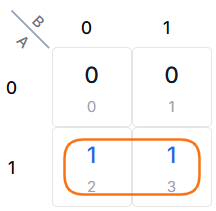
\includegraphics[keepaspectratio]{images/04-boolesk-algebra/K_map_example_2inputs.png}}

\caption{\label{fig-example-with-karnaugh}Karnaughdiagram för
sanningstabellen i Tabell~\ref{tbl-tt-example-with-karnaugh}.}

\end{figure}%

Genom att visualisera sanningstabellen i ett Karnaughdiagram och
identifiera rutor med 1 (SOP, mintermerna) kan man enkelt se att
uttrycket blir 1 när \(A = 1\), oavsett vad \(B\) har för värde. Så
istället för att räkna ut att \(A \cdot B + A \cdot \overline{B} = A\),
ringar vi helt enkelt in två intilliggande ettor i diagrammet för att
göra förenklingen direkt.

\end{tcolorbox}

När vi arbetar med Karnaughdiagram följer vi tre huvudregler:

\begin{enumerate}
\def\labelenumi{\arabic{enumi}.}
\tightlist
\item
  \textbf{Storleken spelar roll:} Vi vill skapa så stora grupper som
  möjligt i multipler av 2 (\(1, 2, 4, 8, 16\)).
\item
  \textbf{Endast närliggande:} Vi får bara ringa in ettor som ligger
  vägg-i-vägg (horisontellt eller vertikalt). Vi letar alltså efter
  rektangulärt formade inringningar.
\item
  \textbf{Inga diagonaler:} Grupper får aldrig bildas diagonalt. Notera!
  XOR och XNOR syns som diagonala ``schackrutemönster'' i ett
  Karnaughdiagram. Karnaughdiagram används alltså för att hitta OR- och
  AND-strukturer.
\end{enumerate}

\begin{tcolorbox}[enhanced jigsaw, arc=.35mm, bottomrule=.15mm, bottomtitle=1mm, breakable, colback=white, colbacktitle=quarto-callout-tip-color!10!white, colframe=quarto-callout-tip-color-frame, coltitle=black, left=2mm, leftrule=.75mm, opacityback=0, opacitybacktitle=0.6, rightrule=.15mm, title=\textcolor{quarto-callout-tip-color}{\faLightbulb}\hspace{0.5em}{Kom ihåg!}, titlerule=0mm, toprule=.15mm, toptitle=1mm]

Karnaughdiagrammet är inte ``platt'' -- det är en yta som hänger ihop.
Den vänstra kanten gränsar mot den högra, och den översta raden gränsar
mot den nedersta. Tänk dig att diagrammet är en torus (en badring) eller
en cylinder!

\end{tcolorbox}

Exemplet ovan har bara två variabler \(A\) och \(B\), så vinsten med att
använda Karnaughdiagram jämfört med sanningstabellen är inte uppenbar.
Fördelarna blir mer tydliga när vi går till tre eller fler variaabler,
vilket beskrivs i de kommande avsnitten.

\subsection{Karnaughdiagram för tre
variabler}\label{karnaughdiagram-fuxf6r-tre-variabler}

När vi går från två till tre variabler (\(A, B, C\)) expanderar vi vår
sanningstabell från 4 till 8 rader. För att kunna förenkla dessa uttryck
visuellt behöver vi ett 3-variablers Karnaughdiagram. Eftersom
Karnaughdiagrammet bara har två variabler kommer två av variablerna slås
samman. Det spelar egentligen ingen roll hur och i denna bok slår vi
samman de två första variablerna och skapar fyra rader i
Karnaughdiagrammet. Det viktigaste att komma ihåg här är att vi måste
bibehålla \textbf{Gray-kod} i den axel där vi har två variabler. Så i
ett 3-variablers diagram lägger vi \(AB\) på raderna och \(C\) på
kolumnerna, se Figur~\ref{fig-Karnaugh-3inputs} (men man kan lika gärna
lägga \(A\) på raderna och \(BC\) på kolumnerna). Lägg märke till
radordningen: \textbf{00, 01, 11, 10}.

\begin{figure}

\pandocbounded{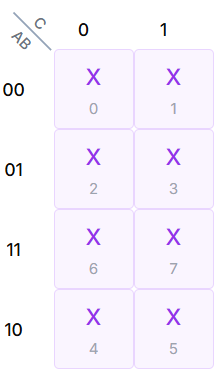
\includegraphics[keepaspectratio]{images/04-boolesk-algebra/K_map_example_3inputs.png}}

\caption{\label{fig-Karnaugh-3inputs}Karnaughdiagram med tre variabler,
\(A\), \(B\) och \(C\). De två första variablerna slås samman och bildar
fyra rader som skrivs med Gray-kod. X kan vara 0 eller 1, men används
också för ``don't care'', vilket beskrivs i Avsnitt~\ref{sec-dont-care}.
I diagrammet finns också ett ordningstal 0 - 7, som representerar
motsvarade decimaltal och därmed radordningen i tillhörande
sanningstabell.}

\end{figure}%

Varför används Gray-kod och en ordning där 11 kommer före före 10? Om vi
hade skrivit 00, 01, 10, 11 så skulle hoppet mellan 01 och 10 kräva att
\textbf{två bitar ändras samtidigt}. I ett Karnaughdiagram får varje
steg bara innebära att \textbf{en enda bit ändras}. Genom att använda
Gray-koden (00 -\textgreater{} 01 -\textgreater{} 11 -\textgreater{} 10)
garanterar vi att vi alltid kan se grannskapen korrekt.

Eftersom vi använder Gray-kod hänger även kolumnerna ihop. Den första
kolumnen (00) och den sista kolumnen (10) betraktas som grannar. Om du
har ettor i båda dessa kan de bilda en grupp tillsammans, trots att de
ser ut att stå på varsin sida om diagrammet.

\begin{tcolorbox}[enhanced jigsaw, arc=.35mm, bottomrule=.15mm, bottomtitle=1mm, breakable, colback=white, colbacktitle=quarto-callout-note-color!10!white, colframe=quarto-callout-note-color-frame, coltitle=black, left=2mm, leftrule=.75mm, opacityback=0, opacitybacktitle=0.6, rightrule=.15mm, title=\textcolor{quarto-callout-note-color}{\faInfo}\hspace{0.5em}{Exempel: Karnaughdiagram med tre ingångar}, titlerule=0mm, toprule=.15mm, toptitle=1mm]

\begin{figure}[H]

\pandocbounded{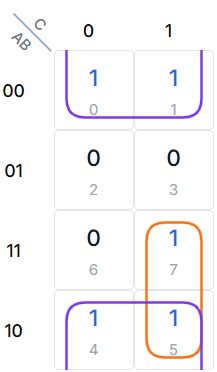
\includegraphics[keepaspectratio]{images/04-boolesk-algebra/K_map_example_3inputs_around_corner.png}}

\caption{\label{fig-Karnaugh-example-with-3inputs}Karnaughdiagram med
tre ingångar.}

\end{figure}%

Ovanstående Karnaughdiagram i
Figur~\ref{fig-Karnaugh-example-with-3inputs} visar ett system med tre
ingångar. Fem olika logiska kombinationer ger logisk 1 på utgången.
Övriga tre kombinationen ger logisk 0.

Med sanningstabell skulle vi få ett ganska långt uttryck med mintermar:

\[Y = \overline{A}\overline{B}\overline{C} + \overline{A}\overline{B}C + A\overline{B}\overline{C} + A\overline{B}C + ABC\]

Att förenkla från detta uttryck tar lite tid, så istället är det mer
effektivt att använda Karnaughdiagrammet. I detta fall så används SOP,
det vill säga identifiering av ettor.

I diagrammet ser vi att vi kan ringa in ett block med fyra ettor
(violett) som ``går runt kanten'' och kopplar samman översta och
understa raderna. Genom att studera denna inringen kan man se att detta
block är 1 när \(B = 0\) och att det inte spelar någon roll vad \(A\)
respektive \(C\) har för värde. Detta block kan alltså skrivas som
\$overline\{B\}. Sedan finns det en etta kvar (i rutan med ordningstalet
7). Denna kan slås samman med ettan som är i rutan med ordningstalet 5,
för att skapa så stor inringning som möjligt (orange). Spelar ingen roll
att denna etta redan är med i violetta inringningen. I arbetet med
Karnaughdiagrammet strävar man alltid efter så stora inringningar som
möjligt. Inringningen med orange färg är 1 när \(C = 1\) och när
\(A = 1\), så den kan representeras som \(A \cdot C\).

Kombineras uttrycken för violett inringning och orange inringning fås
det förenklade uttrycket:

\[Y = \overline{B} + A \cdot C\]

\end{tcolorbox}

\subsection{Karnaughdiagram för fyra
variabler}\label{sec-karnaugh-4inputs}

När vi går från tre till fyra variabler (till exempel \(A, B, C, D\))
dubblas antalet möjliga tillstånd från 8 till 16. Att förenkla dessa
uttryck algebraiskt blir snabbt arbetssamt, men med ett 4-variablers
Karnaughdiagram förblir metoden visuell och intuitiv. Ett
4-variablersdiagram organiseras som en \(4 \times 4\)-matris, se
Figur~\ref{fig-Karnaugh-example-4inputs}. Viktigt att komma ihåg är att
är att använda Gray-kod för båda axlarna (\(00, 01, 11, 10\)). Detta
säkerställer att endast en variabel ändras mellan intilliggande rutor,
vilket är en förutsättning för att mönsterigenkänningen ska fungera.

\begin{figure}

\pandocbounded{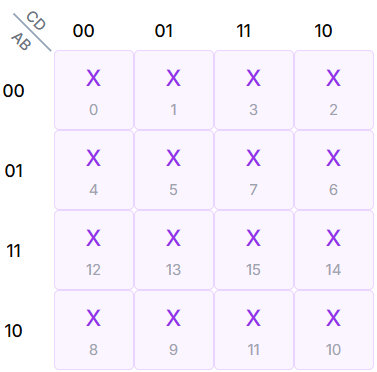
\includegraphics[keepaspectratio]{images/04-boolesk-algebra/K_map_example_4inputs.png}}

\caption{\label{fig-Karnaugh-example-4inputs}Karnaughdiagram med fyra
variabler, \(A\), \(B\), \(C\) och \(D\). Här kombineras variablerna
parvis och bildar fyra rader respektive fyra kolumner (som skrivs med
Gray-kod). .}

\end{figure}%

Med fyra variabler kan vi gruppera ettor i större formationer än
tidigare:

\begin{itemize}
\tightlist
\item
  \textbf{Grupp om 8:} Eliminerar tre variabler (lämnar en variabel
  kvar).
\item
  \textbf{Grupp om 4:} Eliminerar två variabler (lämnar två variabler
  kvar).
\item
  \textbf{Grupp om 2:} Eliminerar en variabel (lämnar tre variabler
  kvar).
\end{itemize}

\begin{tcolorbox}[enhanced jigsaw, arc=.35mm, bottomrule=.15mm, bottomtitle=1mm, breakable, colback=white, colbacktitle=quarto-callout-note-color!10!white, colframe=quarto-callout-note-color-frame, coltitle=black, left=2mm, leftrule=.75mm, opacityback=0, opacitybacktitle=0.6, rightrule=.15mm, title=\textcolor{quarto-callout-note-color}{\faInfo}\hspace{0.5em}{Exempel: Karnaughdiagram för sjusegmentsavkodare, segment \textbf{A}}, titlerule=0mm, toprule=.15mm, toptitle=1mm]

\begin{figure}[H]

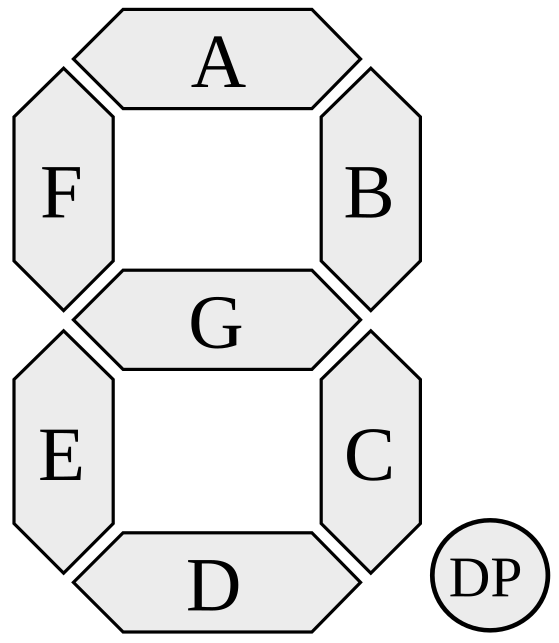
\includegraphics[width=0.15\linewidth,height=\textheight,keepaspectratio]{images/04-boolesk-algebra/7_segment_display_labeled.png}

\caption{\label{fig-7seg-display}Uppbyggnad av en sjusegmentdisplay.
Källa: By user:h2g2bob - Own work ~This W3C-unspecified vector image was
created with Inkscape ., CC BY-SA 3.0,
https://commons.wikimedia.org/w/index.php?curid=1451959.}

\end{figure}%

En sjusegmentsdisplay används ofta för att skapa billig och enkelt
display för att visa siffror 0-9. Men den kan även användas för
hexadecimala tal, men med justeringen att man skriver b respektive d för
att inte blanda samman de hexadecimala tecknen B och D med 8 respektive
0.

En sanningstabell för segment \textbf{A} ser ut som följer. Här
representerar ingångarna \(d3, d2, d1, d0\) de fyra bitarna i det
hexadecimala värdet (0--F). Segment \textbf{A} är utgång:

\begin{longtable}[]{@{}cccccc@{}}
\caption{Sanningstabell för sjusegmentavkodning av segment A för
hexadecimala symboler.}\label{tbl-hex-to-7seg}\tabularnewline
\toprule\noalign{}
Hexsymbol & d3 & d2 & d1 & d0 & Segment \textbf{A} \\
\midrule\noalign{}
\endfirsthead
\toprule\noalign{}
Hexsymbol & d3 & d2 & d1 & d0 & Segment \textbf{A} \\
\midrule\noalign{}
\endhead
\bottomrule\noalign{}
\endlastfoot
0 & 0 & 0 & 0 & 0 & 1 \\
1 & 0 & 0 & 0 & 1 & 0 \\
2 & 0 & 0 & 1 & 0 & 1 \\
3 & 0 & 0 & 1 & 1 & 1 \\
4 & 0 & 1 & 0 & 0 & 0 \\
5 & 0 & 1 & 0 & 1 & 1 \\
6 & 0 & 1 & 1 & 0 & 1 \\
7 & 0 & 1 & 1 & 1 & 1 \\
8 & 1 & 0 & 0 & 0 & 1 \\
9 & 1 & 0 & 0 & 1 & 1 \\
A & 1 & 0 & 1 & 0 & 1 \\
b & 1 & 0 & 1 & 1 & 0 \\
C & 1 & 1 & 0 & 0 & 1 \\
d & 1 & 1 & 0 & 1 & 0 \\
E & 1 & 1 & 1 & 0 & 1 \\
F & 1 & 1 & 1 & 1 & 1 \\
\end{longtable}

Karnaughdiagrammet med fyra insignaler (se
Figur~\ref{fig-Karnaugh-example-4inputs}) ser ut så här:

\begin{figure}[H]

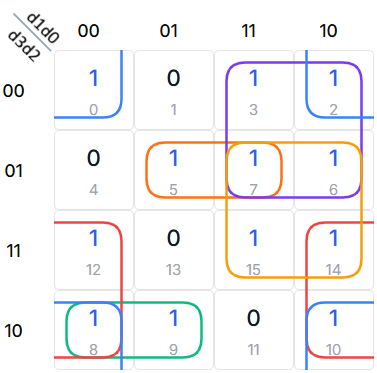
\includegraphics[width=0.4\linewidth,height=\textheight,keepaspectratio]{images/04-boolesk-algebra/K_map_7seg_segment_a_edited.png}

\caption{\label{fig-hex-to-7seg}Karnaughdiagram för sanningstabellen i
Tabell~\ref{tbl-hex-to-7seg}.}

\end{figure}%

Diagrammet ser lite stökigt ut, men genom att följa färgmarkeringen så
ser vi att det finns inringat fyra områden med fyra ettor och två
områden med två ettor. Notera att två av områdena med fyra ettor ``går
över kanten'', blå respektive röd. De totalt sex inringade områden kan
skrivas som (sambanden följer färgmarkeringen i Karnaughduagrammet):

\begin{itemize}
\tightlist
\item
  \(\color{highlight_249_115_022} \overline{d3} \cdot d2 \cdot d0\)
\item
  \(\color{highlight_124_058_237} \overline{d3} \cdot d1\)
\item
  \(\color{highlight_016_185_129} d3 \cdot \overline{d2} \cdot \overline{d1}\)
\item
  \(\color{highlight_239_068_068} d3 \cdot \overline{d0}\)
\item
  \(\color{highlight_059_130_246} \overline{d2} \cdot \overline{d0}\)
\item
  \(\color{highlight_245_158_011} d2 \cdot d1\)
\end{itemize}

Hur läser man ut detta? Se till exempel den gröna inringningen. Där ska
vi ha \(d3 = 1, d2 = 0, d1 = 0\) för att få ettorna inom inringningen.
Sista insignalen \(d0\) spelar ingen roll. Det utläses då som
\(d3 \cdot \overline{d2} \cdot \overline{d1}\). Totala uttrycket för
A-segmentet blir förstås:

\[A = \color{highlight_249_115_022} \overline{d3} \cdot d2 \cdot d0 + \color{highlight_124_058_237} \overline{d3} \cdot d1 + \color{highlight_016_185_129} d3 \cdot \overline{d2} \cdot \overline{d1} + \color{highlight_239_068_068} d3 \cdot \overline{d0} + \color{highlight_059_130_246} \overline{d2} \cdot \overline{d0} + \color{highlight_245_158_011} d2 \cdot d1\]

\end{tcolorbox}

De övriga sex segmenten? De behöver behandlas i var sitt Karnaughdiagram
med de fyra ingångarna q0-q3. Det krävs alltså sju stycken
Karnaughdiagram för att skapa logiken till en sjusegmentsavkodare.

\subsection{``Don't care''-villkor (X)}\label{sec-dont-care}

I många digitala system finns det kombinationer av insignaler som aldrig
kommer att inträffa under normal drift. När vi konstruerar en logisk
krets för dessa fall spelar det ingen roll om utgången blir logisk 0
eller 1 -- kretsen kommer ändå aldrig att hamna i det tillståndet.

Dessa tillstånd kallas för \textbf{``don't care''-villkor} och markeras
i sanningstabeller och Karnaughdiagram med ett \textbf{X} (eller ett
streck).

Det stora pedagogiska och tekniska värdet med ``don't care''-villkor är
att de ger oss \textbf{frihet}. När vi ska minimera en logisk funktion
med hjälp av ett Karnaughdiagram får vi välja att låta varje \textbf{X}
representera antingen en 0:a eller en 1:a, beroende på vad som ger den
största och mest effektiva inringningen.

\begin{itemize}
\tightlist
\item
  Om ett \textbf{X} kan hjälpa oss att skapa en större grupp (t.ex. att
  inkludera det i ett block om fyra istället för ett block om två),
  behandlar vi det som en \textbf{1:a}.
\item
  Om ett \textbf{X} inte bidrar till att förenkla någon inringning,
  behandlar vi det som en \textbf{0:a} och ignorerar det.
\end{itemize}

\begin{tcolorbox}[enhanced jigsaw, arc=.35mm, bottomrule=.15mm, bottomtitle=1mm, breakable, colback=white, colbacktitle=quarto-callout-note-color!10!white, colframe=quarto-callout-note-color-frame, coltitle=black, left=2mm, leftrule=.75mm, opacityback=0, opacitybacktitle=0.6, rightrule=.15mm, title=\textcolor{quarto-callout-note-color}{\faInfo}\hspace{0.5em}{Exempel: Karnaughdiagram för sjusegmentsavkodare för BCD, segment
\textbf{A}}, titlerule=0mm, toprule=.15mm, toptitle=1mm]

I exempelt med sjusegmentsavkodare i för hexadecimala tecken i
Avsnitt~\ref{sec-karnaugh-4inputs} så var Karnaughdiagrammet fyllt med 0
eller 1. Det behövdes eftersom vi skulle skapa logiken för alla 16
varianter av insignaler. Då kunde vi inte ha någon ``don't care''. Men
för en sjusegmentavkodare för BCD och siffrorna 0-9 blir det annorlunda,
då A-F inte ska användas och aldrig kommer förekomma som insignal.

\begin{figure}[H]

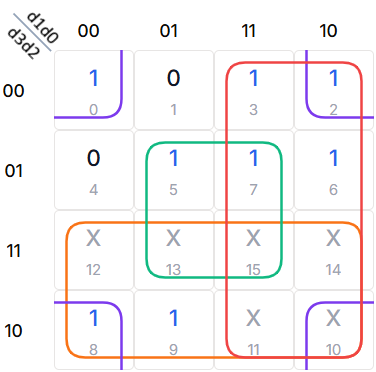
\includegraphics[width=0.4\linewidth,height=\textheight,keepaspectratio]{images/04-boolesk-algebra/K_map_BCD_7seg_segment_a_edited.png}

\caption{\label{fig-BCD-to-7seg}Karnaughdiagram för A-segmentet för en
BCD-till-sjusegmentavkodare.}

\end{figure}%

Nu kan X väljas som 1 eller 0, beroende på vilket som passar bäst. Då
kan ofta större områden ringas in och även färre områden. Här så används
alla X som ettor eftersom det ger bäst resultat (stora och få
inringningar). I detta exempel så har vi nu två områden med åtta ettor
samt två områden med fyra ettor, vilket är betydligt enklare än i
exemplet med full hexadecimal avkodning. Det totala uttrycket blir nu:

\[A = \color{highlight_249_115_022} d3 + \color{highlight_124_058_237} \overline{d2} \cdot \overline{d0} + \color{highlight_016_185_129} d2 \cdot d0 + \color{highlight_239_068_068} d1\]

Uttrycket är nu betydligt enklare än motsvarande uttryck för full
hexadecimal avkodning. Hårdvaruimplementationen blir naturligtvis också
mycket enklare. Detta är styrkan med ``don't care'', de ger större
frihet i designen. Det gäller dock att komma ihåg att om man lägger
något annat än BCD-kod (det vill säga man matar in A-F) så kommer
avkodningen inte stämma.

\end{tcolorbox}

\begin{tcolorbox}[enhanced jigsaw, arc=.35mm, bottomrule=.15mm, bottomtitle=1mm, breakable, colback=white, colbacktitle=quarto-callout-tip-color!10!white, colframe=quarto-callout-tip-color-frame, coltitle=black, left=2mm, leftrule=.75mm, opacityback=0, opacitybacktitle=0.6, rightrule=.15mm, title=\textcolor{quarto-callout-tip-color}{\faLightbulb}\hspace{0.5em}{Behöver alla X hanteras?}, titlerule=0mm, toprule=.15mm, toptitle=1mm]

\textbf{Viktigt att komma ihåg:} Du behöver inte ringa in alla ``don't
care''-X. Ring bara in de som faktiskt hjälper dig att göra dina
inringningar större.

\end{tcolorbox}

\subsection{Karnaughdiagram för fler än fyra
variabler}\label{karnaughdiagram-fuxf6r-fler-uxe4n-fyra-variabler}

Kan man ha fler än fyra variabler? Ja i princip, men då går
Karnaughdiagrammet från en tvådimensionell struktur som kan visas på
skärm eller papper till en flerdimensionell struktur. Med fem respektive
sex ingångar blir det som en tredimensionell struktur, dvs. som en kub.
Det går dock att skära upp kuben i skivor och lägga ut som flera
tvådimensionella diagram, men då behöver man tänka till lite extra för
att kunna ringa in ettorna alternativt nollorna. Detta kräver att man är
mycket noggrann vid inringningen, eftersom man måste ta hänsyn till
grannskap både inom den egna skivan och mellan de två skivorna.

Lyckligtvis finns det onlineverktyg som hjälper till med detta.
https://karnaughmapsolver.com/ som använts för att skapa diagrammen i
denna litteratur har stöd för upp till fem ingångar. Andra verktyg har
ännu fler möjligheter.

\section{SOP och POS: Två sätt att uttrycka logik}\label{sec-SOP-POS}

Tidigare (i Avsnitt~\ref{sec-karnaugh-history}) introducerades begreppen
Sum of Product (SOP) respektive POS (Product of Sums) som två olika sätt
att behandla Karnaughdiagrma. Se exempelvis Figur~\ref{fig-BCD-to-7seg}.
Förenklat innebär det att räkna ettor respektive nollor. När vi ska
implementera en logisk funktion i en krets kan vi som diskuterats
tidigare uttrycka den på två huvudsakliga standardformer, med mintermer
(motsvaras av SOP) eller maxtermer (motsvaras av POS). Valet mellan
dessa beror ofta på hur många ``1:or'' jämfört med ``0:or'' vi har i vår
sanningstabell.

\subsection{SOP (Sum of Products) -- Summan av
produkter}\label{sop-sum-of-products-summan-av-produkter}

SOP är den vanligaste formen när vi arbetar med Karnaughdiagram och det
är den som beskrivits hittills. Den innebär att vi identifierar alla
kombinationer som ger utgången \textbf{logisk 1}.

\begin{itemize}
\tightlist
\item
  \textbf{Logik:} ``Vi tar AND-kombinationer (produkter) av variabler
  och OR:ar ihop dem (summerar dem).''
\item
  \textbf{Användning:} SOP är intuitivt när vi vill veta \emph{när} en
  funktion ska aktiveras.
\item
  \textbf{Notation:} Strukturen för en SOP-form för en funktion \(Y\)
  ser ut som: \[Y = (A \cdot B) + (C \cdot D)\]
\end{itemize}

\subsection{POS (Product of Sums) -- Produkten av
summor}\label{pos-product-of-sums-produkten-av-summor}

POS är den ``omvända'' formen. Här fokuserar vi istället på när utgången
ska vara \textbf{logisk 0}. Vi identifierar dessa rader i
sanningstabellen, skapar OR-villkor (summor) för dem, och AND:ar ihop
dessa grupper.

\begin{itemize}
\tightlist
\item
  \textbf{Logik:} ``Vi skapar OR-kombinationer av variabler och AND:ar
  ihop dem.''
\item
  \textbf{Användning:} POS är ofta mer effektivt om funktionen har
  väldigt få 0:or jämfört med 1:or i sanningstabellen.
\item
  \textbf{Notation:} Strukturen för en POS-form för en funktion \(Y\)
  ser ut som: \[Y = (A + B) \cdot (C + D)\]
\end{itemize}

\begin{tcolorbox}[enhanced jigsaw, arc=.35mm, bottomrule=.15mm, bottomtitle=1mm, breakable, colback=white, colbacktitle=quarto-callout-note-color!10!white, colframe=quarto-callout-note-color-frame, coltitle=black, left=2mm, leftrule=.75mm, opacityback=0, opacitybacktitle=0.6, rightrule=.15mm, title=\textcolor{quarto-callout-note-color}{\faInfo}\hspace{0.5em}{Exempel: Karnaughdiagram för sjusegmentsavkodare för BCD, segment
\textbf{A}, Product of Sums (POS)}, titlerule=0mm, toprule=.15mm, toptitle=1mm]

Vi återanvänder exempelt med sjusegmentsavkodare och segment \textbf{A}
en gång till. I Avsnitt~\ref{sec-dont-care} studerade vi hur man kan
hitta logiska uttrycket för en BCD-till-sjusegmentsavkodare med hjälp av
``don't care''. I det Karnaughdiagrammet var det få nollor, bara två
stycken. Skulle det passa bättre att leta nollor och ringa in dessa?

\begin{figure}[H]

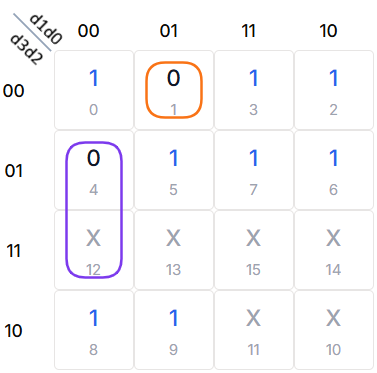
\includegraphics[width=0.4\linewidth,height=\textheight,keepaspectratio]{images/04-boolesk-algebra/K_map_POS_BCD_7seg_segment_a_edited.png}

\caption{\label{fig-Karnaugh-BCD-to-7seg-POS}Karnaughdiagram för
BCD-till-sjusegmentsavkodare och A-segmentet. Här ringas nollor in, det
vill säga uttryck för POS tas fram.}

\end{figure}%

Precis som innan kan X väljas som 1 eller 0, beroende på vilket som
passar bäst. Då kan ofta större områden ringas in och även färre
områden. Här ser vi att det bara blir två områden och i det ena (violett
inringning) vinner vi på att låta X betyda logisk 0, eftersom vi får ett
en större inringning. Inringningen i orange kan nu skrivas som
\(\color{highlight_249_115_022} (d3 + d2 + d1 + \overline{d0})\). d0 är
invers eftersom den är logisk 1 när vi har en utgång som ska vara logisk
0. Inringningen i violett skrivs som
\(\color{highlight_124_058_237} (\overline{d2} + d1 + d0)\). Här spelar
det ingen roll vad d3 har för värde så den utelämnas i uttrycket.

Det totala uttrycket skrivs som produkten av dessa två uttryck:

\[A = \color{highlight_249_115_022} (d3 + d2 + d1 + \overline{d0}) \color{black}{\cdot} \color{highlight_124_058_237} (\overline{d2} + d1 + d0)\]

\end{tcolorbox}

Är de två olika varianterna ekvivalenta och bara två olika sätt att
skriva samma sak? Kan man använda Boolesk algebra för att gå från SOP
till POS och vice versa? I detta fallet så är det inte så, vilket beror
på att vi använt ``don't care''. Studerar vi detaljerna i
Karnaughdiagrammen i respektive exempel ser vi att position 11 i ena
fallet är logisk 1 och i andra fallet logisk 0. Då är de härledda,
förenklade uttrycken inte helt ekvivalenta.Men så länge vi håller oss
till bara BCD-kodade insignaler ser vi ingen skillnad.

\begin{tcolorbox}[enhanced jigsaw, arc=.35mm, bottomrule=.15mm, bottomtitle=1mm, breakable, colback=white, colbacktitle=quarto-callout-tip-color!10!white, colframe=quarto-callout-tip-color-frame, coltitle=black, left=2mm, leftrule=.75mm, opacityback=0, opacitybacktitle=0.6, rightrule=.15mm, title=\textcolor{quarto-callout-tip-color}{\faLightbulb}\hspace{0.5em}{Vilken metod ska man välja?}, titlerule=0mm, toprule=.15mm, toptitle=1mm]

Valet mellan SOP och POS styrs oftast av antalet inringningar som krävs
i ett Karnaughdiagram:

\begin{enumerate}
\def\labelenumi{\arabic{enumi}.}
\tightlist
\item
  \textbf{Ringa in 1:or (SOP):} Om funktionen har få 1:or i
  sanningstabellen är SOP enklast. Det ger direkt stöd för
  AND-OR-implementation.
\item
  \textbf{Ringa in 0:or (POS):} Om funktionen har få 0:or är det
  snabbare att ringa in dessa (vilket ger uttrycket \(\overline{Y}\))
  och sedan använda de Morgans lagar för att invertera resultatet till
  POS-form.
\end{enumerate}

\textbf{Tänk på:} En krets implementerad i POS-form med NAND-grindar
eller NOR-grindar kan ofta bli mer kompakt än en ren
AND-OR-implementation, vilket är en viktig faktor vid design av
integrerade kretsar.

\end{tcolorbox}

\section{Från logiska uttryck till grindar: NAND och
NOR}\label{fruxe5n-logiska-uttryck-till-grindar-nand-och-nor}

I praktiken bygger vi sällan kretsar med en blandning av AND- och
OR-grindar. Istället använder vi nästan uteslutande \textbf{NAND-logik}
eller \textbf{NOR-logik}. Varför? För att dessa grindar är
``universella'' och ofta är både billigare och snabbare att tillverka i
kisel i integrerade kretsar. Det är användbart för man kan nämligen
skapa alla logiska kretsar med uteslutande NAND, alternativt uteslutande
NOR.

I klassiska kretsar i 7400-serien, var NAND en krets som var enkel att
implementera direkt i kisel med BJT-transistor. NAND var då en
grundkrets i själva kiselstrukturen. För att till exempel få en AND
behövdes extra transistor och resistor för att skapa en invertering.
Därmed behövdes mer plats på kiselchipet och det gav också ökade
förluster. I modernare halvledare, som använder MOS-transistorer är NAND
och NOR enklast att implementera, jämfört med andra AND och OR. Därför
finns det goda skäl att tala OM NAND-logik och NOR-logik.

\subsection{NAND-logik (för
SOP/mintermer)}\label{nand-logik-fuxf6r-sopmintermer}

När vi har tagit fram ett uttryck i \textbf{SOP-form} (Sum of Products)
har vi en logisk struktur som ser ut som
\(Y = (A \cdot B) + (C \cdot D)\). Vi har en summa av produkter. Genom
att använda de Morgans lagar kan vi visa att en AND-grind följt av en
OR-grind är logiskt ekvivalent med en struktur av endast NAND-grindar,
se Figur~\ref{fig-NAND-logic}. För att implementera en SOP-funktion med
NAND så genomförs alltså följande steg:

\begin{itemize}
\tightlist
\item
  Ersätt alla AND-grindar med NAND.
\item
  Ersätt OR-grinden i nästa led med en OR där ingångarna är inverterade
  för att kompensera för inverteringen som övergången från AND till NAND
  skapade.
\item
  Ersätt OR-grinden med inverterade ingångar med en NAND (De Morgan).
  Resultatet blir en krets med enhetlig grindtyp (NAND).
\end{itemize}

\begin{figure}

\pandocbounded{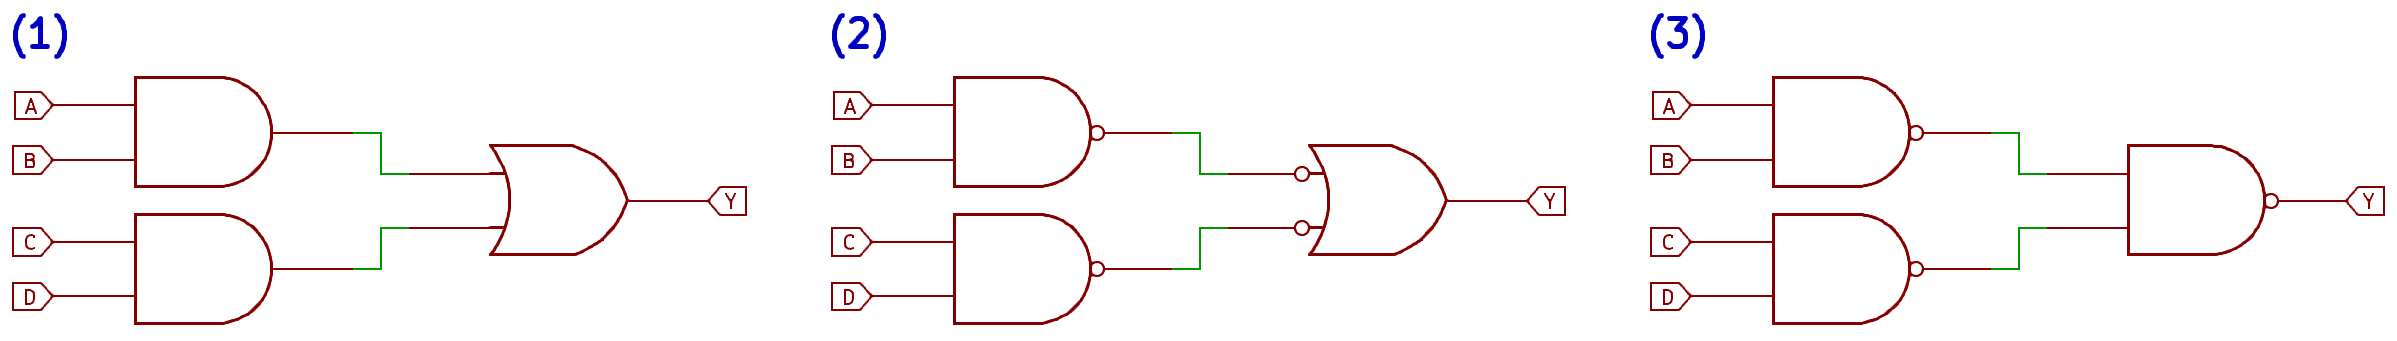
\includegraphics[keepaspectratio]{images/04-boolesk-algebra/NAND_logic.png}}

\caption{\label{fig-NAND-logic}Omvandling av generellt SOP-struktur med
AND-logik för ingångarna som summeras med OR för att få utgången.
\textbf{(1)} visar grundlogiken för SOP,
\(Y = (A \cdot B) + (C \cdot D)\). I \textbf{(2)} ersätts AND med NAND
och då måste ingångarna till OR-grinden inverteras på grund av att en
invertering införts. Denna OR-grind med inverterade ingångar kan med De
Morgans lag skrivas som en NAND, eftersom
\(Y = \overline{A \cdot B} = \overline{A} + \overline{B}\). Slutligen är
vi framme vid schemat i \textbf{(3)} och där har hela logiska kretsen
byggts med tre stycken NAND.}

\end{figure}%

\subsection{NOR-logik (för
POS/Maxtermer)}\label{nor-logik-fuxf6r-posmaxtermer}

När vi arbetar med \textbf{POS-form} (Product of Sums),
\(Y = (A + B) \cdot (C + D)\), är \textbf{NOR-grindar} vårt främsta
verktyg, se Figur~\ref{fig-NOR-logic}. För att implementera en
POS-funktion med NOR så genomförs alltså följande steg:

\begin{itemize}
\tightlist
\item
  Ersätt alla OR-grindar med NOR.
\item
  Ersätt AND-grinden med en AND där ingångarna är inverterade för att
  kompensera för inverteringen som infördes i föregående steg.
\item
  Ersätt AND-grinden med inverterade ingångar med en NOR (De Morgan).
  Resultatet blir en krets med enhetlig grindtyp (NOR).
\end{itemize}

\begin{figure}

\pandocbounded{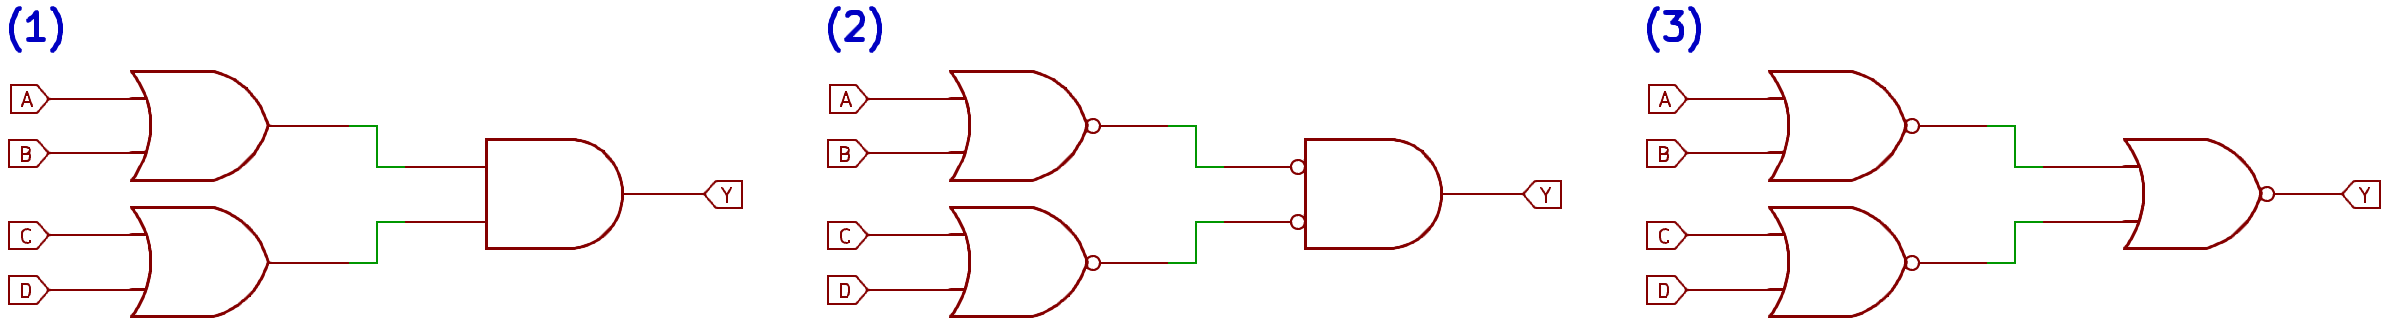
\includegraphics[keepaspectratio]{images/04-boolesk-algebra/NOR_logic.png}}

\caption{\label{fig-NOR-logic}Omvandling av generellt POS-struktur.
\textbf{(1)} visar grundlogiken för POS, \(Y = (A + B) \cdot (C + D)\).
I \textbf{(2)} ersätts OR med NOR och då måste ingångarna till
AND-grinden inverteras på grund av att en invertering införts. Denna
AND-grind med inverterade ingångar kan med De Morgans lag skrivas som en
NOR, eftersom
\(Y = \overline{A + B} = \overline{A} \cdot \overline{B}\). Slutligen är
vi framme vid schemat i \textbf{(3)} och där har hela logiska kretsen
byggts med tre stycken NOR.}

\end{figure}%

\subsection{Sammanfattning: SOP och POS, mintermer och maxtermer,
NAND-logik och
NOR-logik}\label{sammanfattning-sop-och-pos-mintermer-och-maxtermer-nand-logik-och-nor-logik}

För att knyta ihop hela det Booleska kapitlet kan vi se det som två
sidor av samma mynt, se Tabell~\ref{tbl-NAND_NOR_summary}.

\begin{longtable}[]{@{}lll@{}}
\caption{Sammanställning NAND- och NOR-logik samt deras koppling till
min/max och SOP/POS.}\label{tbl-NAND_NOR_summary}\tabularnewline
\toprule\noalign{}
Egenskap & SOP (Mintermer) & POS (Maxtermer) \\
\midrule\noalign{}
\endfirsthead
\toprule\noalign{}
Egenskap & SOP (Mintermer) & POS (Maxtermer) \\
\midrule\noalign{}
\endhead
\bottomrule\noalign{}
\endlastfoot
\textbf{Fokus} & Identifiera 1:or & Identifiera 0:or \\
\textbf{Grindtyp} & AND-OR & OR-AND \\
\textbf{Favoritgrind} & \textbf{NAND} & \textbf{NOR} \\
\textbf{Bäst när\ldots{}} & Funktionen har få 1:or & Funktionen har få
0:or \\
\end{longtable}

Att behärska övergången mellan dessa former och förstå hur man
``NAND-ifierar'' eller ``NOR-ifierar'' sin krets är det som skiljer en
teoretisk logiker från en praktisk hårdvarukonstruktör. Nu när vi har de
logiska grunderna på plats, är vi redo att använda dem för att bygga mer
avancerade komponenter som multiplexrar och räknare.

\bookmarksetup{startatroot}

\chapter{Kombinatoriska kretsar}\label{sec-kombinatoriska-kretsar}

I de tidigare kapitlen har vi bekantat oss med de minsta beståndsdelarna
i digital logik: de enskilda grindarna. Vi har också lärt oss hur vi med
Boolesk algebra och Karnaughdiagram kan optimera dessa för att lösa
specifika logiska problem. Nu är det dags att ta steget från lösa
komponenter till färdiga \textbf{kombinatoriska byggblock}.

\section{Vad är en kombinatorisk
krets?}\label{sec-vad-ar-kombinatoriska-kretsar}

En kombinatorisk krets kännetecknas av att dess utgångar (\(Y\)) vid
varje givet tillfälle \textbf{enbart} beror på de nuvarande värdena på
ingångarna (\(A, B, C \dots\)). Man kan likna det vid en matematisk
funktion \(y = f(x)\); så fort du ändrar \(x\), ändras \(y\) omedelbart
(bortsett från viss fördröjning i hårdvaran).

Det innebär att en kombinatorisk krets:

\begin{itemize}
\tightlist
\item
  \textbf{Saknar minne:} Den har ingen aning om vad ingångarna var för
  en sekund sedan.
\item
  \textbf{Är tidsoberoende:} Den bryr sig inte om i vilken ordning
  signaler anländer, så länge de nuvarande nivåerna är stabila.
\end{itemize}

För att förstå kraften i kombinatorisk logik underlättar det att se vad
den \emph{inte} är. Den andra stora huvudgruppen inom digitalteknik är
\textbf{sekventiella kretsar} (som vi behandlar i senare kapitel). I en
sekventiell krets sparas information, vilket gör att utgången beror både
på vad som skickas in just nu och vad som hände tidigare.

\begin{longtable}[]{@{}
  >{\raggedright\arraybackslash}p{(\linewidth - 4\tabcolsep) * \real{0.3333}}
  >{\raggedright\arraybackslash}p{(\linewidth - 4\tabcolsep) * \real{0.3333}}
  >{\raggedright\arraybackslash}p{(\linewidth - 4\tabcolsep) * \real{0.3333}}@{}}
\caption{Skillnader i egenskaperna hos kombinatoriska kretsar jämfört
med sekventiella
kretsar.}\label{tbl-kombinatoriska_sekventiella}\tabularnewline
\toprule\noalign{}
\begin{minipage}[b]{\linewidth}\raggedright
Egenskap
\end{minipage} & \begin{minipage}[b]{\linewidth}\raggedright
Kombinatoriska kretsar
\end{minipage} & \begin{minipage}[b]{\linewidth}\raggedright
Sekventiella kretsar
\end{minipage} \\
\midrule\noalign{}
\endfirsthead
\toprule\noalign{}
\begin{minipage}[b]{\linewidth}\raggedright
Egenskap
\end{minipage} & \begin{minipage}[b]{\linewidth}\raggedright
Kombinatoriska kretsar
\end{minipage} & \begin{minipage}[b]{\linewidth}\raggedright
Sekventiella kretsar
\end{minipage} \\
\midrule\noalign{}
\endhead
\bottomrule\noalign{}
\endlastfoot
\textbf{Beroende} & Beror endast på nuvarande ingångar. & Beror på
nuvarande ingångar \textbf{och} tidigare tillstånd. \\
\textbf{Minne} & Nej. & Ja (t.ex. vippor). \\
\textbf{Klocka} & Oftast inte (asynkrona). & Oftast klockstyrda
(synkrona). \\
\textbf{Exempel} & Adderare, Multiplexrar, Avkodare. & Räknare,
Register, CPU-styrenheter. \\
\end{longtable}

Kombinatoriska kretsar fungerar alltså som digitalteknikens
``beslutsfattare''. De tar emot ett gäng bitar och spottar direkt ut ett
resultat baserat på en förbestämd logisk struktur. I detta kapitel ska
vi titta på de vanligaste av dessa strukturer: från kretsar som kan
räkna (adderare) till kretsar som kan välja och dirigera data
(multiplexrar).

\section{Logiska nivåer: Active High och Active
Low}\label{sec-active-high-low}

Innan vi går in på specifika komponenter måste vi reda ut ett begrepp
som ofta förvirrar nya inom digitalteknik: \textbf{Active Low}.

I teorin tänker vi oss ofta att en ``1'' betyder PÅ och en ``0'' betyder
AV. Detta kallas för \textbf{Active High} (positiv logik). Men i
praktiken, särskilt när vi arbetar med komponenter i 7400-serien, är det
precis lika vanligt att en funktion aktiveras av en nolla.

\subsection{Vad innebär Active Low?}\label{sec-active-low}

En signal som är \textbf{Active Low} (negativ logik) anses vara ``sann''
eller ``aktiv'' när spänningen är låg (0 V). När spänningen är hög (5 V
alternativt 3.3 V) är funktionen inaktiv.

\begin{itemize}
\tightlist
\item
  \textbf{Active High:} 0 = Inaktiv, 1 = Aktiv.
\item
  \textbf{Active Low:} 1 = Inaktiv, 0 = Aktiv.
\end{itemize}

\subsection{Hur identifierar man Active
Low?}\label{sec-hur-identifiera-active-low}

I teknisk dokumentation och kopplingsscheman kan du känna igen Active
Low på två tydliga sätt:

\begin{enumerate}
\def\labelenumi{\arabic{enumi}.}
\tightlist
\item
  \textbf{Cirkeln (Inverteringsbubblan):} Om du ser en liten ring vid en
  ingång eller utgång på en logiksymbol betyder det att signalen
  inverteras där. En ring på en \emph{Enable}-ingång betyder alltså att
  kretsen startar när den får en nolla. I äldre datablad kan man ibland
  se en triangel i stället för en ring.
\item
  \textbf{Namngivningen:} Signaler som är Active Low skrivs ofta med ett
  streck över namnet (\(\overline{Reset}\)), ett prefix (nReset) eller
  ett suffix (Reset\_L eller Reset\#).
\end{enumerate}

\subsection{Varför krångla till det?}\label{sec-varfor-active-low}

Det finns flera tekniska anledningar till att Active Low är
industristandard:

\begin{itemize}
\tightlist
\item
  \textbf{Robusthet:} Det är ofta enklare och säkrare att dra en signal
  till jord (GND) för att aktivera något.
\item
  \textbf{Elektrisk strömstyrka:} Äldre digitalteknikkretsar (TTL) var
  konstruerad så att kretsarna var mycket bättre på att ``sänka'' ström
  (\textbf{sink}, ta emot ström till jord) än att ``skicka ut'' ström
  (\textbf{source}). Det kan ha betydelse om något ska drivas av
  digitalkretsen.
\item
  \textbf{Wired-OR:} Det underlättar när flera olika kretsar ska kunna
  dra i samma ``nödbroms'' (t.ex. en gemensam Reset-lina) utan att
  kortsluta varandra. Genom att använda Active Low och Open
  Collector-utgångar kan flera enheter dela på samma ledning.
\end{itemize}

\begin{tcolorbox}[enhanced jigsaw, arc=.35mm, bottomrule=.15mm, bottomtitle=1mm, breakable, colback=white, colbacktitle=quarto-callout-important-color!10!white, colframe=quarto-callout-important-color-frame, coltitle=black, left=2mm, leftrule=.75mm, opacityback=0, opacitybacktitle=0.6, rightrule=.15mm, title=\textcolor{quarto-callout-important-color}{\faExclamation}\hspace{0.5em}{Tips när du kopplar på breadboard eller felsöker din kretskortsdesign}, titlerule=0mm, toprule=.15mm, toptitle=1mm]

Kontrollera om komponenten du har problem med använder Active Low. Att
missa detta är ett av de vanligaste felen vid koppling av digitala
kretsar!

\end{tcolorbox}

\section{Enable: Kretsens huvudströmbrytare}\label{sec-enable}

Många kretsar i 7400-serien har en eller flera ingångar som kallas för
\textbf{Enable} (förkortat \textbf{EN}, \textbf{E} eller ibland
\textbf{G} för \emph{Gate}). Detta fungerar som en logisk strömbrytare
för hela komponenten.

\subsection{Varför behövs Enable?}\label{varfuxf6r-behuxf6vs-enable}

I ett digitalt system delar ofta många olika kretsar på samma ledningar
(en så kallad \emph{buss}). Om alla kretsar skulle skicka ut data
samtidigt skulle det uppstå kortslutningar eller datakonflikter.

Enable-pinnen tillåter oss att:

\begin{enumerate}
\def\labelenumi{\arabic{enumi}.}
\tightlist
\item
  \textbf{Välja komponent:} Vi kan ha tio olika avkodare i ett system
  men låta bara en av dem vara ``vaken'' åt gången.
\item
  \textbf{Spara energi:} I vissa teknologier drar kretsen mindre ström
  när den är inaktiverad.
\item
  \textbf{Synkronisera:} Vi kan ställa in alla ingångar i lugn och ro
  och sedan ``slå på'' kretsen precis när vi vill att resultatet ska
  visas.
\end{enumerate}

\begin{itemize}
\tightlist
\item
  \textbf{När Enable är aktiv:} Kretsen fungerar normalt och följer sin
  sanningstabell.
\item
  \textbf{När Enable är inaktiv:} Kretsen ignoreras. Utgångarna går
  oftast till ett fast inaktivt läge (eller blir ``flytande'' i
  högimpedans-läge).
\end{itemize}

\subsection{Identifiera Enable i
scheman}\label{identifiera-enable-i-scheman}

Precis som med logiska nivåer i Avsnitt~\ref{sec-varfor-active-low}, är
Enable-signaler väldigt ofta \textbf{Active Low}.

\begin{itemize}
\tightlist
\item
  \textbf{Active High (\(EN\) / \(G\)):} Kretsen aktiveras av en logisk
  \textbf{1:a} (5V).
\item
  \textbf{Active Low (\(\overline{E}\) / \(\overline{G}\)):} Kretsen
  aktiveras av en logisk \textbf{0:a} (0V/GND). Denna känns igen på
  ringen vid ingången eller strecket över namnet.
\end{itemize}

\subsection{Sammansatt Enable}\label{sammansatt-enable}

Vissa kretsar kräver att flera villkor är uppfyllda samtidigt för att
starta. Ett klassiskt exempel är 3-till-8-avkodaren \textbf{74LS138}.
Den har tre Enable-pinnar:

\begin{itemize}
\tightlist
\item
  \textbf{G1} (Active High)
\item
  \textbf{\(\overline{G2A}\)} (Active Low)
\item
  \textbf{\(\overline{G2B}\)} (Active Low)
\end{itemize}

För att kretsen ska fungera måste G1 vara hög \textbf{SAMTIDIGT} som
både \(\overline{G2A}\) och \(\overline{G2B}\) är låga. Detta är mycket
användbart när man vill bygga ut systemet (kaskadkoppla) utan att behöva
lägga till extra logikgrindar.

\begin{tcolorbox}[enhanced jigsaw, arc=.35mm, bottomrule=.15mm, bottomtitle=1mm, breakable, colback=white, colbacktitle=quarto-callout-important-color!10!white, colframe=quarto-callout-important-color-frame, coltitle=black, left=2mm, leftrule=.75mm, opacityback=0, opacitybacktitle=0.6, rightrule=.15mm, title=\textcolor{quarto-callout-important-color}{\faExclamation}\hspace{0.5em}{Tips från labbet: ``Död'' krets?}, titlerule=0mm, toprule=.15mm, toptitle=1mm]

Om du har kopplat in- och utgångar rätt men din krets inte ger något
utslag på utgångarna, är det nästan alltid Enable-pinnen som spökar. Kom
ihåg att en Active Low Enable-pinne \textbf{inte} får lämnas oansluten
(``hängande'') -- den måste kopplas fysiskt till jord för att kretsen
ska vakna!

\end{tcolorbox}

\section{Aritmetiska kretsar: Adderaren}\label{sec-adderaren}

Grunden i all digital beräkning är förmågan att addera två binära tal.
För att bygga en fungerande adderare börjar vi med den enklaste
komponenten: \textbf{Halvadderaren}.

\subsection{Halvadderaren (Half-Adder)}\label{sec-halv-adderaren}

En halvadderare kan lägga ihop två bitar, \(A\) och \(B\), och leverera
en summa (\(S\)) samt en minnessiffra, så kallad ``carry out''
(\(C_{out}\)).

\begin{longtable}[]{@{}llll@{}}
\caption{Sanningstabell för \textbf{halvadderare}. Halvadderaren har två
utgångar, en som visar summan och en som visar minnessiffran
(carry).}\label{tbl-halvadderare}\tabularnewline
\toprule\noalign{}
A & B & Summa (S) & Carry (C) \\
\midrule\noalign{}
\endfirsthead
\toprule\noalign{}
A & B & Summa (S) & Carry (C) \\
\midrule\noalign{}
\endhead
\bottomrule\noalign{}
\endlastfoot
0 & 0 & 0 & 0 \\
0 & 1 & 1 & 0 \\
1 & 0 & 1 & 0 \\
1 & 1 & 0 & 1 \\
\end{longtable}

Som vi ser i Tabell~\ref{tbl-halvadderare} motsvaras summan \(S\) av en
\textbf{XOR}-funktion och carry-signalen \(C\) av en
\textbf{AND}-funktion. Detta är realiserat i övre kretsschemat i
Figur~\ref{fig-half-adder-full-adder}.

\begin{figure}

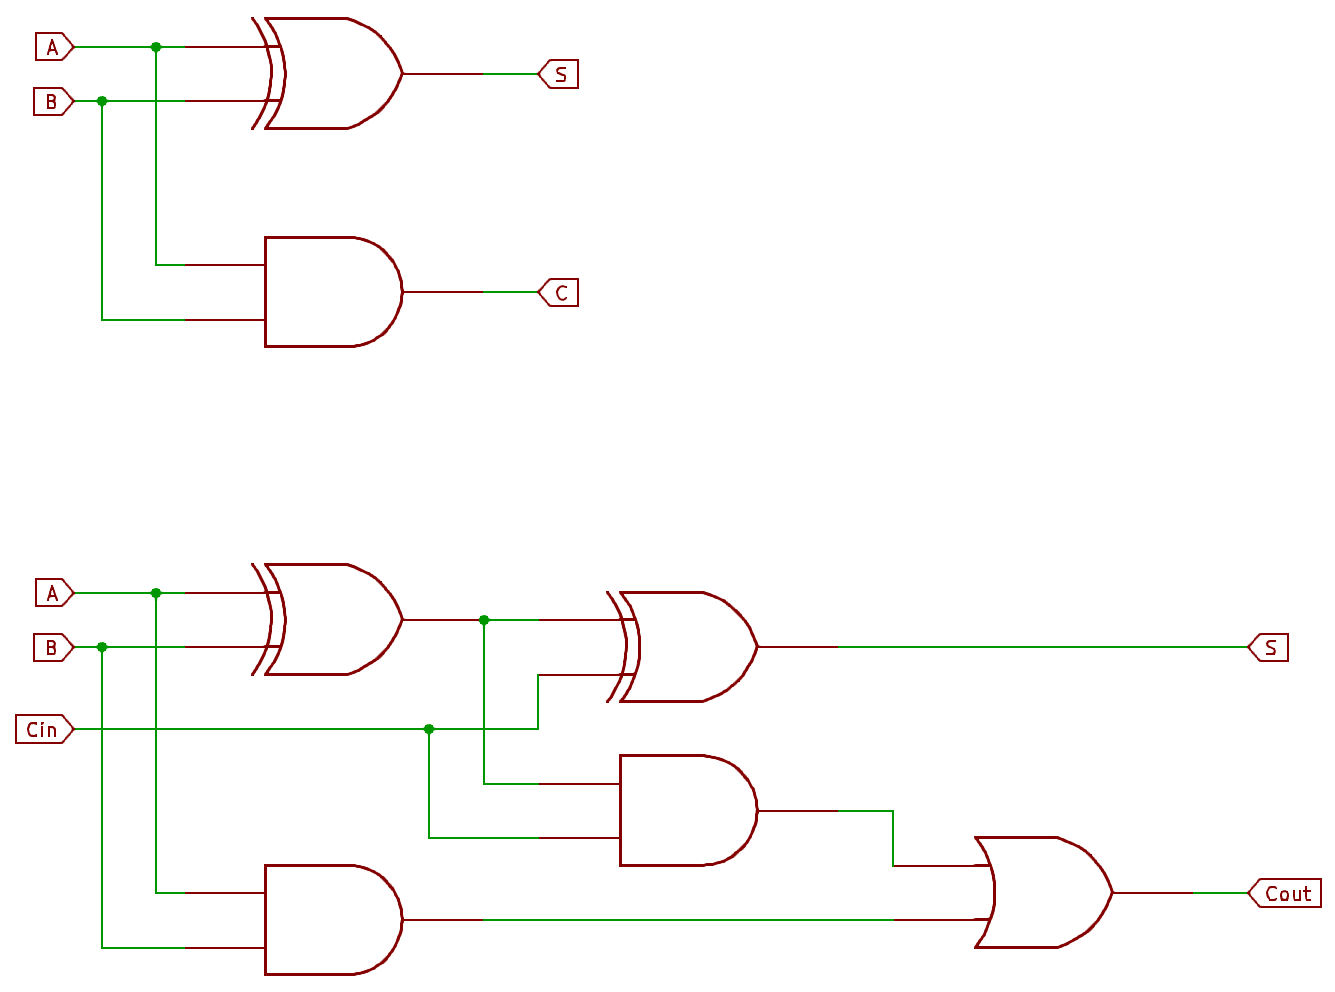
\includegraphics[width=0.5\linewidth,height=\textheight,keepaspectratio]{images/05-kombinatoriska-kretsar/half_adder_full_adder.png}

\caption{\label{fig-half-adder-full-adder}Halvadderare överst (half
adder) och heladderare underst (full adder), realiserade med logiska
grindar.}

\end{figure}%

\subsection{Heladderaren (Full-Adder)}\label{sec-heladderaren}

Begränsningen med en halvadderare är att den bara kan hantera två bitar.
När vi adderar flersiffriga tal för hand skriver vi ofta en
``minnessiffra'' ovanför nästa kolumn. I digitaltekniken kallas detta
för en \textbf{Carry In} (\(C_{in}\)). Minnessiffran blir då en tredje
bit som ska ingå i summeringen.

En \textbf{heladderare} har därför tre ingångar: \(A\), \(B\) och
\(C_{in}\). Den levererar precis som tidigare en summa (\(S\)) och en
carry-out (\(C_{out}\)).

\begin{longtable}[]{@{}ccccc@{}}
\caption{Sanningstabell för \textbf{heladderare}. Heladderaren hanterar
tre ingångar så att addition med minnessiffra kan
genomföras.}\label{tbl-heladderare}\tabularnewline
\toprule\noalign{}
\(A\) & \(B\) & \(C_{in}\) & Summa (\(S\)) & \(C_{out}\) \\
\midrule\noalign{}
\endfirsthead
\toprule\noalign{}
\(A\) & \(B\) & \(C_{in}\) & Summa (\(S\)) & \(C_{out}\) \\
\midrule\noalign{}
\endhead
\bottomrule\noalign{}
\endlastfoot
0 & 0 & 0 & 0 & 0 \\
0 & 1 & 0 & 1 & 0 \\
1 & 0 & 0 & 1 & 0 \\
1 & 1 & 0 & 0 & 1 \\
0 & 0 & 1 & 1 & 0 \\
0 & 1 & 1 & 0 & 1 \\
1 & 0 & 1 & 0 & 1 \\
1 & 1 & 1 & 1 & 1 \\
\end{longtable}

En heladderare kan realiseras genom att kombinera två halvadderare och
en OR-grind, se undre kretsschemat i
Figur~\ref{fig-half-adder-full-adder}. Den första halvadderaren lägger
ihop \(A\) och \(B\). Den andra halvadderaren lägger sedan ihop
resultatet med \(C_{in}\). Om någon av halvadderarna genererar en carry,
skickas den vidare via OR-grinden som \(C_{out}\).

\subsection{Parallelladderare (Ripple Carry
Adder)}\label{sec-parallelladderaren}

För att addera binära tal med fler än en bit, till exempel två 4-bitars
tal (\(A_{3}A_{2}A_{1}A_{0}\) och \(B_{3}B_{2}B_{1}B_{0}\)), kopplar man
samman flera heladderare i en kedja.

Denna struktur kallas ofta för en \textbf{Ripple Carry Adder} eftersom
carry-signalen måste ``rippla'' (fortplanta sig) genom varje steg, från
den minst signifikanta biten (LSB) till den mest signifikanta biten
(MSB).

\begin{tcolorbox}[enhanced jigsaw, arc=.35mm, bottomrule=.15mm, bottomtitle=1mm, breakable, colback=white, colbacktitle=quarto-callout-note-color!10!white, colframe=quarto-callout-note-color-frame, coltitle=black, left=2mm, leftrule=.75mm, opacityback=0, opacitybacktitle=0.6, rightrule=.15mm, title=\textcolor{quarto-callout-note-color}{\faInfo}\hspace{0.5em}{Exempel: 3-bitars Ripple Carry Adder}, titlerule=0mm, toprule=.15mm, toptitle=1mm]

En 3-bitars adderare kan skapas med en halvadderare för LSB (position 0,
det vill säga \(2^0\)), följt av två stycken heladderare som hanterar
positionernna 1 respektive 2. Heladderare behövs för att kunna hantera
eventuella ``minnessiffror'' i additionen. Det går självklart lika bra
att bygga med tre stycken heladderare och sätta första carry-signalen
\(C_{0,in} = 0\).

\begin{figure}[H]

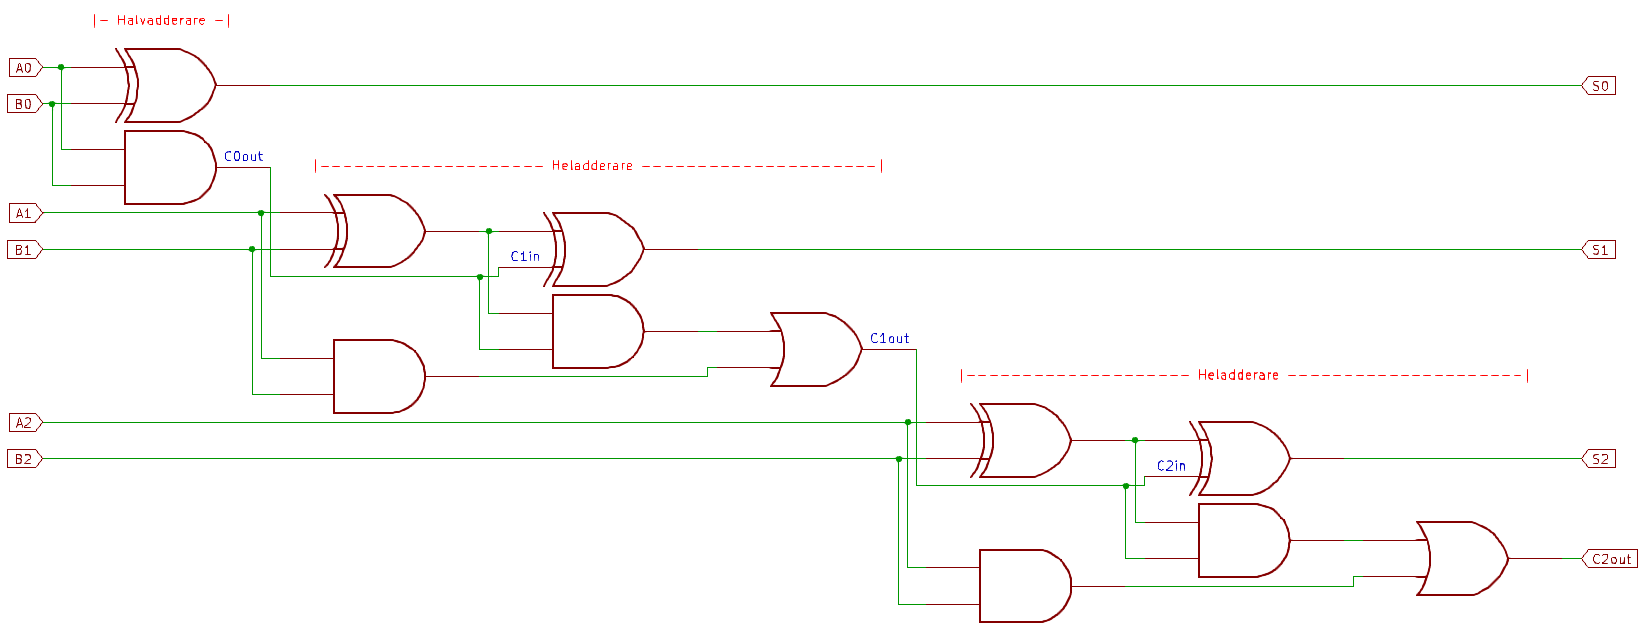
\includegraphics[width=0.9\linewidth,height=\textheight,keepaspectratio]{images/05-kombinatoriska-kretsar/3bit-adder.png}

\caption{\label{fig-3bit-adder}3-bitars adderare realiserad med en
halvadderare följd av två heladderare.}

\end{figure}%

\end{tcolorbox}

\subsubsection{Carry Look-Ahead (CLA) -- Snabbare
addition}\label{sec-carry-look-ahead}

Även om Ripple Carry-adderaren är enkel att förstå och bygga, har den en
stor nackdel i system som kräver snabba beräkningar:
\textbf{tidsfördröjning}.

Varje grind i kretsen tar några nanosekunder på sig att reagera. Innan
den sista biten adderas (MSB) i en adderare kan visa ett korrekt värde,
måste carry-signaler från tidigare additioner ha vandrat genom alla
föregående steg. Ju fler bitar vi adderar, desto långsammare blir
kretsen. För att lösa problemet med fördröjningen i en Ripple
Carry-adderare används \textbf{Carry Look-Ahead}. Istället för att vänta
på att carry-signalen ska vandra (rippla) genom varje steg, beräknar man
i förväg om en carry kommer att skapas.

Tekniken bygger på två logiska begrepp för varje bit-position (\(i\)):

\begin{enumerate}
\def\labelenumi{\arabic{enumi}.}
\tightlist
\item
  \textbf{Generate (\(G_i\)):} En carry skapas (genereras) i detta steg
  om både \(A_i\) och \(B_i\) är 1. \[G_i = A_i \cdot B_i\]
\item
  \textbf{Propagate (\(P_i\)):} En inkommande carry kommer att skickas
  vidare (propageras) till nästa steg om antingen \(A_i\) eller \(B_i\)
  är 1. \[P_i = A_i + B_i\] (eller ofta \(A_i \oplus B_i\) för att spara
  logik)
\end{enumerate}

Genom att använda dessa två funktioner kan vi skriva uttrycket för carry
ut (\(C_{out}\)) från vilken bit som helst utan att behöva veta vad
föregående steg har kommit fram till än.

För den första biten (\(C_1\)) ser det ut som vanligt:
\[C_1 = G_0 + (P_0 \cdot C_{in})\]

Men för den andra biten (\(C_2\)) kan vi sätta in formeln för \(C_1\)
direkt:
\[C_2 = G_1 + P_1(G_0 + P_0 \cdot C_{in}) = G_1 + P_1 G_0 + P_1 P_0 C_{in}\]

\textbf{Slutsats:} Som vi ser i formeln för \(C_2\) beror resultatet nu
bara på de ursprungliga ingångarna (\(A, B\) och \(C_{in}\)) och inte på
den faktiska beräkningen i steget innan. Alla carry-signaler kan alltså
beräknas \textbf{samtidigt} i en separat logikkrets (Carry Look-ahead
Unit). Detta gör adderaren extremt mycket snabbare, men på bekostnad av
att kretsen blir betydligt mer komplex och kräver fler grindar.

\subsection{Subtraktion: Adderaren som gör
allt}\label{sec-subtraheraren}

I digitalteknik bygger vi sällan specifika kretsar för subtraktion.
Istället utnyttjar vi matematiken bakom \textbf{tvåkomplement}. För att
beräkna \(A - B\) gör vi istället om det till en addition: \(A + (-B)\).

För att skapa \(-B\) (tvåkomplementet av \(B\)) behöver vi göra två
saker: 1. Invertera alla bitar i \(B\) (NOT). 2. Addera 1 till
resultatet.

En generell adderare/subtraherare kan implemeneteras genom att lägga
till en styrsignal \(Sub\). Då kan vi styra om kretsen ska addera eller
subtrahera:

\begin{itemize}
\tightlist
\item
  \textbf{XOR som kontrollerbar inverterare:} Varje bit i talet \(B\)
  körs genom en XOR-grind tillsammans med \(Sub\)-signalen.

  \begin{itemize}
  \tightlist
  \item
    Om \(Sub = 0\): Bitarna passerar oförändrade (\(B \oplus 0 = B\)).
  \item
    Om \(Sub = 1\): Bitarna inverteras (\(B \oplus 1 = \overline{B}\)).
  \end{itemize}
\item
  \textbf{Carry-in tricket:} Genom att koppla \(Sub\)-signalen direkt
  till adderarens första \textbf{Carry-in} (\(C_{in}\)), får vi den där
  ``extra adderade ettan'' som krävs för tvåkomplementet helt gratis när
  \(Sub=1\).
\end{itemize}

Detta är extremt effektivt. Med bara några extra XOR-grindar har vi
skapat en enhet som kan hantera både addition och subtraktion, vilket
sparar både plats och ström i processorn.

\section{Datadirigering: Multiplexern (mux)}\label{sec-multiplexern}

Efter att ha tittat på hur vi räknar med data, ska vi nu se hur vi
väljer vilken data som ska skickas var. Den viktigaste komponenten för
detta är \textbf{multiplexern}, ofta förkortad \textbf{mux} (eller
\textbf{MUX}). En multiplexer fungerar som en digital strömbrytare eller
en växeltavla. Den har flera dataingångar men bara \textbf{en} utgång.
Vilken av ingångarna som kopplas till utgången bestäms av en eller flera
\textbf{styrsignaler} (Select-lines). Motsatsen till en multiplexer är
\textbf{demultiplexern}, som tar en ingång med data och fördelar till
flera utgångar.

\subsection{2-till-1 multiplexer}\label{sec-2-till-1-multiplexer}

Den enklaste multiplexern har två dataingångar (\(D_0, D_1\)) och en
styrsignal (\(S\)).

\begin{itemize}
\tightlist
\item
  Om \(S = 0\), kopplas \(D_0\) till utgången.
\item
  Om \(S = 1\), kopplas \(D_1\) till utgången.
\end{itemize}

Detta är en fundamental byggsten som används överallt i datorarkitektur
för att styra dataflöden mellan olika register och enheter.

Hur ser en multiplexer ut på insidan? För en 2-till-1 MUX kan vi
beskriva funktionen med ett logiskt uttryck. Om \(Y\) är utgången, \(S\)
är styrsignalen och \(D_0, D_1\) är dataingångarna, blir uttrycket:

\(Y = (\overline{S} \cdot D_0) + (S \cdot D_1)\).

Detta innebär att om \(S=0\), blir den högra termen noll och \(Y\) styrs
helt av \(D_0\). Om \(S=1\), blir den vänstra termen noll och \(Y\)
styrs av \(D_1\). Se även Tabell~\ref{tbl-2-to-1-multiplexer}.

\begin{longtable}[]{@{}ccccl@{}}
\caption{Sanningstabell för en 2-till-1
multiplexer.}\label{tbl-2-to-1-multiplexer}\tabularnewline
\toprule\noalign{}
\(S\) (Styr) & \(D_1\) & \(D_0\) & \textbf{\(Y\) (Ut)} & Beskrivning \\
\midrule\noalign{}
\endfirsthead
\toprule\noalign{}
\(S\) (Styr) & \(D_1\) & \(D_0\) & \textbf{\(Y\) (Ut)} & Beskrivning \\
\midrule\noalign{}
\endhead
\bottomrule\noalign{}
\endlastfoot
0 & 0 & \textbf{0} & \textbf{0} & \(S=0\), utgången följer \(D_0\) \\
0 & 0 & \textbf{1} & \textbf{1} & \(S=0\), utgången följer \(D_0\) \\
0 & 1 & \textbf{0} & \textbf{0} & \(S=0\), utgången följer \(D_0\) \\
0 & 1 & \textbf{1} & \textbf{1} & \(S=0\), utgången följer \(D_0\) \\
1 & \textbf{0} & 0 & \textbf{0} & \(S=1\), utgången följer \(D_1\) \\
1 & \textbf{0} & 1 & \textbf{0} & \(S=1\), utgången följer \(D_1\) \\
1 & \textbf{1} & 0 & \textbf{1} & \(S=1\), utgången följer \(D_1\) \\
1 & \textbf{1} & 1 & \textbf{1} & \(S=1\), utgången följer \(D_1\) \\
\end{longtable}

Styrsignalen kommer alltså bestämma om \(D0\) eller \(D1\) når utgången.

\subsection{Större multiplexrar
(n-till-1)}\label{sec-n-till-1-multiplexer}

När vi vill välja mellan fler än två ingångar behöver vi fler
styrsignaler. Antalet ingångar (\(n\)) bestämmer hur många styrbitar
(\(s\)) som krävs enligt sambandet \(n = 2^s\).

Som exempel kan vi studera en \textbf{4-till-1 multiplexer}. Den har
fyra ingångar \(D_0 - D_3\) och kräver alltså 2 styrbitar
(\(S_1, S_0\)).

\begin{longtable}[]{@{}ccc@{}}
\caption{Förenklad sanningstabell för en 4-till-1
multiplexer.}\label{tbl-4-to-1-multiplexer}\tabularnewline
\toprule\noalign{}
\(S_1\) & \(S_0\) & Utgång (Y) \\
\midrule\noalign{}
\endfirsthead
\toprule\noalign{}
\(S_1\) & \(S_0\) & Utgång (Y) \\
\midrule\noalign{}
\endhead
\bottomrule\noalign{}
\endlastfoot
0 & 0 & \(D_0\) \\
0 & 1 & \(D_1\) \\
1 & 0 & \(D_2\) \\
1 & 1 & \(D_3\) \\
\end{longtable}

Implementeringen med grindlogik görs på motsvarande sätt som för
2-till-1 multiplexern.

\[Y = (\overline{S_1} \cdot \overline{S_0} \cdot D_0) + (\overline{S_1} \cdot S_0 \cdot D_1) + (S_1 \cdot \overline{S_0} \cdot D_2) + (S_1 \cdot S_0 \cdot D_3)\]

Varje term i parentes representerar en unik kombination av
styrsignalerna:

\begin{itemize}
\tightlist
\item
  \textbf{Term 1:} Om \(S_1=0\) och \(S_0=0\), aktiveras den första
  AND-grinden och släpper igenom \(D_0\).
\item
  \textbf{Term 2:} Om \(S_1=0\) och \(S_0=1\), aktiveras den andra
  AND-grinden och släpper igenom \(D_1\).
\item
  \textbf{Term 3:} Om \(S_1=1\) and \(S_0=0\), aktiveras den tredje
  AND-grinden och släpper igenom \(D_2\).
\item
  \textbf{Term 4:} Om \(S_1=1\) och \(S_0=1\), aktiveras den fjärde
  AND-grinden och släpper igenom \(D_3\).
\end{itemize}

\subsection{Praktisk tillämpning:
Databusstyrning}\label{praktisk-tilluxe4mpning-databusstyrning}

I en enkel processor används multiplexrar för att bestämma vilket värde
som ska skickas till räkneenheten (ALU:n). Ska det vara ett värde från
ett register, eller ska det vara ett tal som kommer direkt från
programkoden? En MUX fattar beslutet baserat på instruktionen som
processorn just nu läser.

\section{Demultiplexern (demux)}\label{demultiplexern-demux}

Om multiplexern är en väljare som samlar in data, är
\textbf{demultiplexern} dess spegelbild eller motsats. Den tar
\textbf{en} dataingång och skickar vidare den till \textbf{en av flera}
utgångar.

Vilken utgång som tar emot datan bestäms, precis som hos mux:en, av
styrsignaler (Select-lines).

\subsection{1-till-2 Demultiplexer}\label{till-2-demultiplexer}

Den enklaste varianten har en dataingång (\(D\)), en styrsignal (\(S\))
och två utgångar (\(Y_0, Y_1\)). Till skillnad från multiplexern, som
har en enda utgångsekvation, har demultiplexern en separat ekvation för
varje utgång. Varje utgång styrs av en unik kombination av
styrsignalerna.

\begin{itemize}
\tightlist
\item
  Om \(S = 0\), kopplas \(D\) till utgång \(Y_0\). (Utgång \(Y_1\) blir
  0).
\item
  Om \(S = 1\), kopplas \(D\) till utgång \(Y_1\). (Utgång \(Y_0\) blir
  0).
\end{itemize}

De logiska uttrycken för utgångarna blir: \[Y_0 = D \cdot \overline{S}\]
\[Y_1 = D \cdot S\]

Vid fler än två utgångar tillkommer det styrsignaler på liknande sätt
som för multiplexern.

\begin{tcolorbox}[enhanced jigsaw, arc=.35mm, bottomrule=.15mm, bottomtitle=1mm, breakable, colback=white, colbacktitle=quarto-callout-note-color!10!white, colframe=quarto-callout-note-color-frame, coltitle=black, left=2mm, leftrule=.75mm, opacityback=0, opacitybacktitle=0.6, rightrule=.15mm, title=\textcolor{quarto-callout-note-color}{\faInfo}\hspace{0.5em}{Exempel: 1-till-4 demultimplexer}, titlerule=0mm, toprule=.15mm, toptitle=1mm]

För en DeMUX med fyra utgångar krävs två stycken styrsignaler. Dessa
kombineras med insignalen i AND-grind för att fördela insignalen till
rätt kanal.

\begin{longtable}[]{@{}ccccccl@{}}
\caption{Förenklad sanningstabell för en 1-till-4 demultiplexer. \(D\)
är ingången med data.}\label{tbl-1-till-4-demux}\tabularnewline
\toprule\noalign{}
\(S_1\) & \(S_0\) & \(Y_3\) & \(Y_2\) & \(Y_1\) & \(Y_0\) & Vald
utgång \\
\midrule\noalign{}
\endfirsthead
\toprule\noalign{}
\(S_1\) & \(S_0\) & \(Y_3\) & \(Y_2\) & \(Y_1\) & \(Y_0\) & Vald
utgång \\
\midrule\noalign{}
\endhead
\bottomrule\noalign{}
\endlastfoot
0 & 0 & 0 & 0 & 0 & \textbf{D} & \(Y_0 = D\) \\
0 & 1 & 0 & 0 & \textbf{D} & 0 & \(Y_1 = D\) \\
1 & 0 & 0 & \textbf{D} & 0 & 0 & \(Y_2 = D\) \\
1 & 1 & \textbf{D} & 0 & 0 & 0 & \(Y_3 = D\) \\
\end{longtable}

För att realisera detta i hårdvara använder vi fyra AND-grindar med tre
ingångar vardera:

\begin{itemize}
\tightlist
\item
  \(Y_0 = D \cdot \overline{S_1} \cdot \overline{S_0}\)
\item
  \(Y_1 = D \cdot \overline{S_1} \cdot S_0\)
\item
  \(Y_2 = D \cdot S_1 \cdot \overline{S_0}\)
\item
  \(Y_3 = D \cdot S_1 \cdot S_0\)
\end{itemize}

Om dataingången \(D\) hålls konstant på logisk etta (\(1\)), fungerar
kretsen precis som en \textbf{2-till-4 Avkodare (Decoder)}. Avkodare är
något som diskuteras i Avsnitt~\ref{sec-avkodare}.

\end{tcolorbox}

\subsection{Systemet med mux och demux som en
helhet}\label{systemet-med-mux-och-demux-som-en-helhet}

I praktiska system, som t.ex. inom telekommunikationssystem eller inuti
en dator, arbetar multiplexern och demultiplexern ofta i par. En mux
``packar ihop'' data från flera källor till en enda ledning
(serialisering), och en demux i andra änden ``packar upp'' datan till
rätt mottagare igen. Detta sparar ledningar i kommunikationsbussarna då
flera datakällor kan samasas om en seriell kommunikationskanal istället
för flera parallella.

\section{Avkodare (Decoders)}\label{sec-avkodare}

En \textbf{avkodare} är en kombinatorisk krets som har \(n\) ingångar
och upp till \(2^n\) utgångar. Dess huvudsakliga uppgift är att
identifiera (avkoda) den binära kombinationen på ingången genom att
aktivera \textbf{en} unik utgång, eller \textbf{en unik kombination} av
utgångar. Ett exempel på användningsområde är inuti en dator eller
mikrokontroller där avkodare kan användas för \textbf{adressavkodning}.
Vissa processorer och arkitekturer har bara en adressbuss men flera
olika komponenter (RAM, ROM, I/O-portar) som är kopplade till bussen, så
här används en avkodare för att välja vilken komponent som ska
``lyssna''.

Man kan se avkodaren som motsatsen till en enkodare, eller som en
demultiplexer där dataingången är fastlåst till en logisk etta.

\subsection{\texorpdfstring{Binäravkodaren
(n-till-\(2^n\))}{Binäravkodaren (n-till-2\^{}n)}}\label{binuxe4ravkodaren-n-till-2n}

Binäravkodaren är en vanlig typ av avkodaren. Ett exempel är
\textbf{2-till-4 avkodare} med 2 bitar in och 4 utgångar. Endast den
utgång som motsvarar ingångens decimalvärde blir hög (1), medan alla
andra förblir låga (0).

\begin{longtable}[]{@{}ccccccl@{}}
\caption{Binäravkodaren för 2
bitar.}\label{tbl-2-till-4-avkodare}\tabularnewline
\toprule\noalign{}
\(A_1\) & \(A_0\) & \(Y_3\) & \(Y_2\) & \(Y_1\) & \(Y_0\) & Vald
utgång \\
\midrule\noalign{}
\endfirsthead
\toprule\noalign{}
\(A_1\) & \(A_0\) & \(Y_3\) & \(Y_2\) & \(Y_1\) & \(Y_0\) & Vald
utgång \\
\midrule\noalign{}
\endhead
\bottomrule\noalign{}
\endlastfoot
0 & 0 & 0 & 0 & 0 & \textbf{1} & \(Y_0\) (noll) \\
0 & 1 & 0 & 0 & \textbf{1} & 0 & \(Y_1\) (ett) \\
1 & 0 & 0 & \textbf{1} & 0 & 0 & \(Y_2\) (två) \\
1 & 1 & \textbf{1} & 0 & 0 & 0 & \(Y_3\) (tre) \\
\end{longtable}

Implementeringen av en binäravkodare är i praktiken en samling
\textbf{AND-grindar} där varje grind är ``programmerad'' med hjälp av
inverterare för att känna igen en unik binär kombination.

För en 2-till-4 avkodare med ingångarna \(A_1\) (MSB) och \(A_0\) (LSB)
ser de booleska uttrycken för utgångarna ut enligt följande:

\begin{itemize}
\tightlist
\item
  \(Y_0 = \overline{A_1} \cdot \overline{A_0}\) (Aktiv när \(A = 00_2\))
\item
  \(Y_1 = \overline{A_1} \cdot A_0\) (Aktiv när \(A = 01_2\))
\item
  \(Y_2 = A_1 \cdot \overline{A_0}\) (Aktiv när \(A = 10_2\))
\item
  \(Y_3 = A_1 \cdot A_0\) (Aktiv när \(A = 11_2\))
\end{itemize}

\textbf{Enable-ingången (EN):} De flesta kommersiella avkodare (t.ex.
74138) har en ``Enable''-pinne. Om EN = 0 är alla utgångar låga, oavsett
vad som finns på ingångarna. Detta används för att styra när en viss del
av ett system ska vara aktivt.

\subsection{BCD-till-decimal-avkodare
(1-av-10)}\label{sec-BCD-decimal-avkodare}

En \textbf{BCD-till-decimal-avkodare} (ofta kallad ``1-av-10-avkodare'')
är en specialiserad variant av binäravkodaren. Den är designad för att
arbeta med \textbf{BCD (Binary Coded Decimal)}, vilket innebär att den
endast tolkar de binära kombinationerna som motsvarar siffrorna 0 till
9.

Ett klassiskt exempel på denna typ av krets i 7400-serien är
\textbf{74LS42}. Kretsen har 4 ingångar (\(A, B, C, D\)) och 10 utgångar
(\(Y_0\) till \(Y_9\)).

\begin{enumerate}
\def\labelenumi{\arabic{enumi}.}
\tightlist
\item
  Om ingången är ett binärtal mellan \texttt{0000} (0) och \texttt{1001}
  (9), aktiveras motsvarande utgång.
\item
  Om ingången är ett tal mellan \texttt{1010} (10) och \texttt{1111}
  (15), betraktas detta som en ``ogiltig'' BCD-kod. I detta läge förblir
  \textbf{samtliga} utgångar inaktiva.
\end{enumerate}

Viktigt att notera med 74LS42 och många andra avkodare är att de
använder \textbf{Active Low}-logik på utgångarna (se
Avsnitt~\ref{sec-active-low}). Det innebär att:

\begin{itemize}
\tightlist
\item
  Den valda utgången går låg (\textbf{0V}).
\item
  De nio icke-valda utgångarna förblir höga (\textbf{5V}).
\end{itemize}

\begin{longtable}[]{@{}
  >{\centering\arraybackslash}p{(\linewidth - 6\tabcolsep) * \real{0.2778}}
  >{\centering\arraybackslash}p{(\linewidth - 6\tabcolsep) * \real{0.2778}}
  >{\raggedright\arraybackslash}p{(\linewidth - 6\tabcolsep) * \real{0.2222}}
  >{\raggedright\arraybackslash}p{(\linewidth - 6\tabcolsep) * \real{0.2222}}@{}}
\caption{Förenklad sanningstabell för BCD-till-decimal-avkodare (Active
Low)}\tabularnewline
\toprule\noalign{}
\begin{minipage}[b]{\linewidth}\centering
Decimalt
\end{minipage} & \begin{minipage}[b]{\linewidth}\centering
BCD-kod (D C B A)
\end{minipage} & \begin{minipage}[b]{\linewidth}\raggedright
Aktiv utgång (Låg)
\end{minipage} & \begin{minipage}[b]{\linewidth}\raggedright
Alla andra utgångar
\end{minipage} \\
\midrule\noalign{}
\endfirsthead
\toprule\noalign{}
\begin{minipage}[b]{\linewidth}\centering
Decimalt
\end{minipage} & \begin{minipage}[b]{\linewidth}\centering
BCD-kod (D C B A)
\end{minipage} & \begin{minipage}[b]{\linewidth}\raggedright
Aktiv utgång (Låg)
\end{minipage} & \begin{minipage}[b]{\linewidth}\raggedright
Alla andra utgångar
\end{minipage} \\
\midrule\noalign{}
\endhead
\bottomrule\noalign{}
\endlastfoot
0 & 0 0 0 0 & \textbf{\(Y_0\)} & Höga \\
1 & 0 0 0 1 & \textbf{\(Y_1\)} & Höga \\
2 & 0 0 1 0 & \textbf{\(Y_2\)} & Höga \\
3 & 0 0 1 1 & \textbf{\(Y_3\)} & Höga \\
4 & 0 1 0 0 & \textbf{\(Y_4\)} & Höga \\
5 & 0 1 0 1 & \textbf{\(Y_5\)} & Höga \\
6 & 0 1 1 0 & \textbf{\(Y_6\)} & Höga \\
7 & 0 1 1 1 & \textbf{\(Y_7\)} & Höga \\
8 & 1 0 0 0 & \textbf{\(Y_8\)} & Höga \\
9 & 1 0 0 1 & \textbf{\(Y_9\)} & Höga \\
10--15 & \textgreater{} 1 0 0 1 & \textbf{Ingen} & Samtliga är Höga \\
\end{longtable}

Dessa kretsar används ofta i äldre kontrollsystem eller för att styra
specifika indikatorer där man vill visa en siffra i taget, men inte
nödvändigtvis på en 7-segmentsdisplay. Ett klassiskt exempel är drivning
av \textbf{Nixie-rör}, där varje utgång från avkodaren tänder en
specifik siffra inuti gasröret.

\subsection{BCD till
7-segmentsavkodare}\label{sec-BCD-till-7seg-avkodare}

En mycket vanlig avkodningstillämpning är att omvandla ett binärtal (BCD
- Binary Coded Decimal) till signaler som kan styra en sifferdisplay. En
\textbf{7-segmentsdisplay} består av sju lysdioder (segment) namngivna
\(A\) till \(G\) (se Figur~\ref{fig-7seg-display}).

Avkodaren (t.ex. kretsen 7447) tar 4 bitar in (decimala värdet 0--9) och
aktiverar de segment som krävs för att rita siffran. Till skillnad från
en binäravkodare kan här \textbf{flera utgångar vara aktiva samtidigt}.

\begin{itemize}
\tightlist
\item
  \textbf{Exempel:} För att visa siffran ``1'' aktiveras segment \(B\)
  och \(C\). För siffran ``8'' aktiveras samtliga segment
  \(A, B, C, D, E, F, G\).
\end{itemize}

\begin{tcolorbox}[enhanced jigsaw, arc=.35mm, bottomrule=.15mm, bottomtitle=1mm, breakable, colback=white, colbacktitle=quarto-callout-warning-color!10!white, colframe=quarto-callout-warning-color-frame, coltitle=black, left=2mm, leftrule=.75mm, opacityback=0, opacitybacktitle=0.6, rightrule=.15mm, title=\textcolor{quarto-callout-warning-color}{\faExclamationTriangle}\hspace{0.5em}{Viktigt: 7447/7448 stöder inte Hexadecimala tal (A--F)}, titlerule=0mm, toprule=.15mm, toptitle=1mm]

En vanlig missuppfattning är att alla 7-segmentsavkodare kan visa
hexadecimala tecken. De klassiska kretsarna i 7400-serien, som
\textbf{7447} och \textbf{7448}, är renodlade \textbf{BCD-avkodare}.

Det innebär att de endast är designade för att visa siffrorna
\textbf{0--9}. Om du skickar in ett binärt värde högre än 9 (t.ex.
\(1010_2\) för `A') kommer displayen inte att visa bokstaven A. Istället
händer något av följande:

\begin{itemize}
\tightlist
\item
  Displayen visar ett märkligt mönster som ser ut som en felaktig
  siffra.
\item
  Displayen släcks helt (blanking).
\end{itemize}

Om ditt projekt kräver att du visar hexadecimala värden (0--F) behöver
du istället använda en mikrokontroller med en programvarubaserad
``lookup-table'' eller en mer specialiserad (och ovanligare) krets som
\textbf{MC14495}.

\end{tcolorbox}

\section{Enkodare (Encoders)}\label{sec-enkodare}

En enkodare utför den omvända operationen av en avkodare. Den har
\(2^n\) ingångar och \(n\) utgångar. Om en av ingångarna aktiveras,
skickar enkodaren ut den binära koden för den ingången.

\subsection{Olika typer av enkodare}\label{olika-typer-av-enkodare}

Precis som med avkodare finns det olika varianter beroende på vad
utgången ska representera:

\begin{itemize}
\tightlist
\item
  \textbf{Binär enkodare (8-till-3):} Den vanligaste typen. Den har 8
  ingångar och översätter den aktiva ingången till ett 3-bitars binärtal
  (000 till 111). Ett exempel är \textbf{74LS148}.
\item
  \textbf{BCD-enkodare (10-till-4):} Denna används ofta för knappsatser.
  Den har 9 ingångar (1--9) och skapar en 4-bitars BCD-kod på utgången.
  Om ingen knapp trycks in tolkar kretsen det som 0. Ett exempel är
  \textbf{74LS147}.
\end{itemize}

Värt att notera är att nästan alla prioritetenkodare i 7400-serien (som
74148 och 74147) använder \textbf{Active Low} på både ingångar och
utgångar.

\begin{itemize}
\tightlist
\item
  För att aktivera ingång 7 måste du dra den till \textbf{jord (0V)}.
\item
  Om ingång 7 är aktiv kommer utgången att visa \texttt{000} (inverterat
  \(111_2\)).
\end{itemize}

Detta kan kännas bakvänt i början, men det beror på skäl som
diskuterades i Avsnitt~\ref{sec-varfor-active-low}.

\subsection{Prioritetsenkodaren (Priority
Encoder)}\label{prioritetsenkodaren-priority-encoder}

En vanlig utmaning med enklare enkodare är: \emph{Vad händer om två
knappar trycks in samtidigt?} Utan extra logik skulle utgången bli en
trasig blandning av båda knapparnas koder.

Lösningen är \textbf{prioritetsenkodaren}. Den är konstruerad så att om
flera ingångar är aktiva samtidigt, så är det ingången med det
\textbf{högsta värdet} som bestämmer utgången. Om både ingång 2 och
ingång 5 aktiveras, kommer utgången att visa koden för 5 (\(101_2\)). De
flesta enkodare i 7400-serien är av denna typ.

En praktisk tillämpning är i en mikrokontroller och interrupthantering.
Mikrokontrollern kan flera externa enheter (t.ex. en sensor, ett
tangentbord och en timer) som vill ha processorns uppmärksamhet
samtidigt. En prioritetsenkodare ser till att den viktigaste händelsen
(avbrottet) hanteras först genom att skicka dess unika kod till
processorn.

\subsection{Kontrollsignaler: GS och
EO}\label{kontrollsignaler-gs-och-eo}

Eftersom enkodare ofta används i större system har de två viktiga
hjälpsignaler som du inte hittar på en avkodare:

\begin{enumerate}
\def\labelenumi{\arabic{enumi}.}
\tightlist
\item
  \textbf{GS (Group Select):} Denna pinne går låg så fort \emph{någon}
  av ingångarna är aktiv. Detta är avgörande, eftersom utgången
  \texttt{000} annars skulle kunna betyda både ``Knapp 0 är tryckt'' och
  ``Ingen knapp alls är tryckt''. GS-pinnen talar om för oss att datan
  på utgången är giltig.
\item
  \textbf{EO (Enable Output):} Denna används för att kaskadkoppla
  (seriekoppla) flera enkodare. Om ingen ingång är aktiv på den första
  enkodaren, skickar den en signal till nästa enkodare att den får lov
  att ta över.
\end{enumerate}

\subsection{Jämförelse: Avkodare vs
Enkodare}\label{juxe4mfuxf6relse-avkodare-vs-enkodare}

Det är lättast att komma ihåg skillnaden genom att se dem som
översättare: * \textbf{Avkodare (Decoder):} Översätter en ``tät''
binärkod till en specifik signal (t.ex. välj rad 5 i minnet). *
\textbf{Enkodare (Encoder):} Översätter en specifik signal till en
``tät'' binärkod (t.ex. knapp 5 trycktes ner).

\section{Komparatorn (Magnitude
Comparator)}\label{komparatorn-magnitude-comparator}

En komparator är en logisk krets som jämför två binära tal, \(A\) och
\(B\), och avgör förhållandet mellan dem. Den har oftast tre utgångar
som indikerar om:

\begin{itemize}
\tightlist
\item
  \(A > B\) (A är större än B)
\item
  \(A < B\) (A är mindre än B)
\item
  \(A = B\) (A är lika med B)
\end{itemize}

\subsection{1-bitskomparatorn}\label{bitskomparatorn}

För att förstå logiken kan vi titta på den enklaste formen av jämförelse
mellan två bitar, \(A\) och \(B\).

\textbf{Lika med-logik (\(A = B\)):} Två bitar är lika om båda är \(0\)
eller båda är \(1\). Detta känns igen som en \textbf{XNOR}-funktion:
\[F_{A=B} = \overline{A \oplus B} = AB + \overline{A}\overline{B}\]

\textbf{Större än-logik (\(A > B\)):} \(A\) är större än \(B\) endast om
\(A=1\) och \(B=0\): \[F_{A>B} = A\overline{B}\]

\textbf{Mindre än-logik (\(A < B\)):} \(A\) är mindre än \(B\) endast om
\(A=0\) och \(B=1\): \[F_{A<B} = \overline{A}B\]

\subsection{Flerbitarskomparatorer
(N-bit)}\label{flerbitarskomparatorer-n-bit}

När vi jämför större tal, till exempel två 4-bitars tal
\(A \, (A_3 A_2 A_1 A_0)\) och \(B \, (B_3 B_2 B_1 B_0)\), arbetar
kretsen enligt en hierarkisk ordning:

\begin{enumerate}
\def\labelenumi{\arabic{enumi}.}
\tightlist
\item
  Den börjar med att jämföra de mest signifikanta bitarna
  (\textbf{MSB}), alltså \(A_3\) och \(B_3\).
\item
  Om \(A_3 > B_3\), så är hela talet \(A > B\), oavsett vad de andra
  bitarna är.
\item
  Om \(A_3 = B_3\), går den vidare och kollar på \(A_2\) och \(B_2\),
  och så vidare.
\item
  Först om alla bitar är identiska aktiveras utgången \(A = B\).
\end{enumerate}

\begin{tcolorbox}[enhanced jigsaw, arc=.35mm, bottomrule=.15mm, bottomtitle=1mm, breakable, colback=white, colbacktitle=quarto-callout-tip-color!10!white, colframe=quarto-callout-tip-color-frame, coltitle=black, left=2mm, leftrule=.75mm, opacityback=0, opacitybacktitle=0.6, rightrule=.15mm, title=\textcolor{quarto-callout-tip-color}{\faLightbulb}\hspace{0.5em}{Visste du?}, titlerule=0mm, toprule=.15mm, toptitle=1mm]

En vanlig standardkrets för detta ändamål är \textbf{74LS85}. Det är en
4-bits magnitudkomparator som dessutom har ``kaskadingångar''. Dessa gör
det möjligt att koppla ihop flera 4-bitskretsar för att jämföra 8, 12
eller 16 bitar.

\end{tcolorbox}

\subsection{Praktiska tillämpningar}\label{praktiska-tilluxe4mpningar}

Komparatorer finns överallt där ett digitalt värde ska styra en
händelse:

\begin{itemize}
\tightlist
\item
  \textbf{Termostater:} Jämför ett börvärde (inställd temp) med ett
  ärvär
\end{itemize}

\bookmarksetup{startatroot}

\chapter{Sekventiella kretsar -- Logik med
minne}\label{sec-sekventiella-kretsar}

Hittills har vi bara arbetat med \textbf{logiska grindar} och hur dessa
kan byggas samman till \textbf{kombinatoriska kretsar}. I dessa bestäms
utgångens värde \emph{enbart} av de nuvarande insignalerna. Så fort du
ändrar en ingång, ändras utgången (efter en kort grindfördröjning). Det
finns ingen historia och inget minne.

\textbf{Sekventiella kretsar} fungerar annorlunda. Det är kretsar som
har någon form av minne. Det betyder att utgångens värde är en
konsekvens av både insignaler och kretsens tidigare historik. Man kan se
det som att tidigare utsignal faktiskt fungerar som en insignal. Det är
faktiskt precis så som man löser minnesfunktionaliteten i sekventiella
kretsar. Genom att återkoppla en utgång till en ingång skapar vi kretsar
som ``minns'' vad som hände nyss. Detta är grunden för digitalt
lagringsutrymme, från enkla register till RAM-minnen.

\begin{itemize}
\tightlist
\item
  \textbf{Kombinatorik:} \(Y = f(\text{Ingångar})\)
\item
  \textbf{Sekventiell logik:}
  \(Y = f(\text{Ingångar, Tidigare tillstånd})\)
\end{itemize}

\section{Latchar (Nivåstyrda minneselement)}\label{sec-latchar}

En \textbf{latch} är den enklaste formen av minne. Den kallas ofta för
``genomskinlig'' (transparent) eftersom den ändrar sitt tillstånd så
fort ingångarna ändras, förutsatt att den är aktiverad.

\subsection{SR-latchen (Set-Reset)}\label{sr-latchen-set-reset}

Den mest grundläggande latchen är SR-latchen. Den har två ingångar:

\begin{enumerate}
\def\labelenumi{\arabic{enumi}.}
\tightlist
\item
  \textbf{S (Set):} Sätter utgången \(Q\) till 1.
\item
  \textbf{R (Reset):} Nollställer utgången \(Q\) till 0.
\end{enumerate}

Den har också oftast två utgångar: \(Q\) och dess invers
\(\overline{Q}\). Värt att notera, latch kallas \emph{nivåstyrd vippa}
med ett svenskt uttryck. Men det finns stor risk för sammanblandning med
det som heter vippa (engelska: flip-flop) som har en likartad men ändå
lite annorlunda funktion. Detta kommer vi se senare i @vippor. För att
undvika sammanblandning används här det engelska begreppet latch och
inte det svenska nivåstyrd vippa. Men det kan vara bra att veta att det
slarvas mycket med begreppen när det gäller dessa grundbyggblock inom
sekventiell logik. Många kallar även latchar för vippor.

\begin{figure}

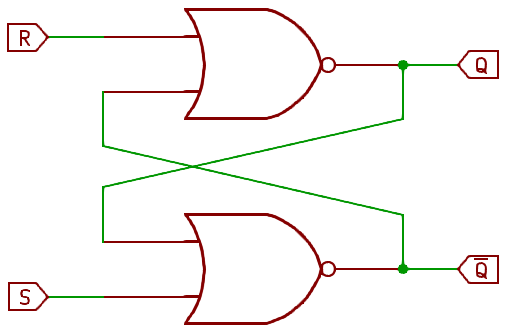
\includegraphics[width=0.5\linewidth,height=\textheight,keepaspectratio]{images/06-sekventiella-kretsar/SR_latch_with_NOR.png}

\caption{\label{fig-SR-latch-with-NOR}SR-latch uppbyggd av två
NOR-grindar. \(S\) (set) sätter latchens utgång \(Q\), medan \(R\)
(reset) nollställer den. Utgången \(\overline{Q}\) är helt enkelt
inversen av \(Q\).}

\end{figure}%

Kretsschemat i Figur~\ref{fig-SR-latch-with-NOR} visar hur man korsvis
återkopplar NOR-grindarnas utgångarna till ingångarna. På så sätt skapas
grunden för minnesfunktionen, och digitalteknikens enklaste latch
(SR-latchen) är född. Sanningstabellen för denna krets visas i
Tabell~\ref{tbl-SR-latch-NOR}.

\begin{longtable}[]{@{}ccccl@{}}
\caption{Sanningstabell för NOR-baserad
SR-latch.}\label{tbl-SR-latch-NOR}\tabularnewline
\toprule\noalign{}
S & R & \(Q\) & \(\overline{Q}\) & Kommentar \\
\midrule\noalign{}
\endfirsthead
\toprule\noalign{}
S & R & \(Q\) & \(\overline{Q}\) & Kommentar \\
\midrule\noalign{}
\endhead
\bottomrule\noalign{}
\endlastfoot
0 & 0 & \(Q_0\) & \(\overline{Q_0}\) & \textbf{Minne:} Ingen ändring
sker. \\
0 & 1 & 0 & 1 & \textbf{Reset:} Utgången nollställs. \\
1 & 0 & 1 & 0 & \textbf{Set:} Utgången sätts till ett. \\
1 & 1 & 0* & 0* & \textbf{Förbjudet:} Båda utgångarna blir noll. \\
\end{longtable}

\begin{tcolorbox}[enhanced jigsaw, arc=.35mm, bottomrule=.15mm, bottomtitle=1mm, breakable, colback=white, colbacktitle=quarto-callout-note-color!10!white, colframe=quarto-callout-note-color-frame, coltitle=black, left=2mm, leftrule=.75mm, opacityback=0, opacitybacktitle=0.6, rightrule=.15mm, title=\textcolor{quarto-callout-note-color}{\faInfo}\hspace{0.5em}{Praktiskt exempel: Status-låsning (Event Capture)}, titlerule=0mm, toprule=.15mm, toptitle=1mm]

I inbyggda system kan vissa händelser vara extremt korta, till exempel
en spänningsspik från en kritisk sensor eller en kortvarig
varningssignal från en motorstyrenhet. Om processorn är upptagen med en
annan tidskritisk uppgift (som att skicka data över ett nätverk) kan den
missa att pinnen blinkade till.

Genom att använda en \textbf{SR-latch} kan vi ``fånga'' händelsen:

\begin{enumerate}
\def\labelenumi{\arabic{enumi}.}
\tightlist
\item
  \textbf{Set:} Den korta fel-signalen kopplas till \(S\)-ingången. Så
  fort felet uppstår sätts latchen och utgången \(Q\) går hög -- och
  \textbf{stannar där}.
\item
  \textbf{Poll:} Processorn kan nu i lugn och ro läsa av pinnen när den
  har tid och se att ``något har hänt'' (att \(Q=1\)).
\item
  \textbf{Reset:} När processorn har registrerat felet skickar den en
  kort puls från en GPIO-pinne till latchens \(R\)-ingång för att
  nollställa den och göra den redo för nästa händelse.
\end{enumerate}

Detta fungerar som ett enkelt hårdvaruminne som avlastar mjukvaran från
att behöva övervaka och läsa av pinnen hela tiden (så kallad polling).
Detta är då ett alternativ till att arbeta med interrupt.

\end{tcolorbox}

Som Tabell~\ref{tbl-SR-latch-NOR} indikerar är tillståndet \(S=1, R=1\)
problematiskt. Om båda ingångarna går höga (\(1\)) så kommer båda
utgångarna bli låga (\(0\)). Det blir motsägelsefullt eftersom utgången
\(\overline{Q}\) är definierad som inversen av \(Q\). Men det stora
problemet uppkommer om båda ingångarna sedan slår om till låg signal
samtidigt för att gå till minnestillståndet, efter att ha varit höga. Då
kan kretsen hamna i ett läge där den ``tävlar'' om vilket värde den ska
ha på utgångarna.

\begin{enumerate}
\def\labelenumi{\arabic{enumi}.}
\tightlist
\item
  Start med \(S=1, R=1\): Båda utgångarna är \(0\).
\item
  Förändring: Vi tar bort båda ettorna på ingångarna samtidigt och
  sätter dessa till nollor.
\item
  Kapplöpningen (race condition): Båda NOR-grindarna ser nu nollor på
  båda sina ingångar och ``tävlar'' om att bli först med att skicka ut
  en etta.
\item
  Den som vinner skickar ut en etta som kommer in på den andra
  NOR-grindens ingång. Denna grind kommer då lägga ut en nolla enligt
  sanningstabellen i Tabell~\ref{tbl-SR-latch-NOR} .
\item
  Resultatet: Den grind som är bråkdelen av en nanosekund snabbare
  vinner.
\end{enumerate}

Men om de är ``exakt'' lika snabba? Då hamnar vi under en tid i det som
kallas i \textbf{metastabilitet}. Kretsen står och väger och har
spänningsnivåer som ligger någonstans mellan låg respektive hög
spänning. Transitorerna, som bygger upp de logiska grindarna, är vare
sig stängda (av) eller öppna (på) utan är halvöppna.

SR-latchen kan även byggas med två NAND-grindar, se
Figur~\ref{fig-SR-latch-with-NAND} och Tabell~\ref{tbl-SR-latch-NAND}.
Den stora skillnaden blir att latchen nu styrs med signaler som är
aktivt låga istället. Det betecknas med \(\overline{S}\) och
\(\overline{R}.\)

\begin{figure}

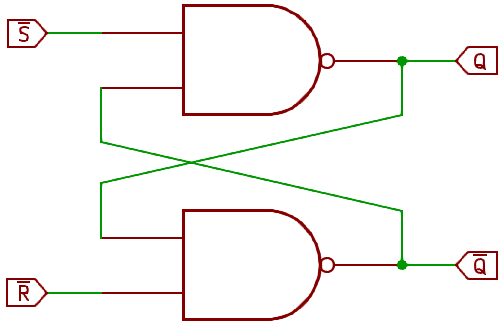
\includegraphics[width=0.5\linewidth,height=\textheight,keepaspectratio]{images/06-sekventiella-kretsar/SR_latch_with_NAND.png}

\caption{\label{fig-SR-latch-with-NAND}SR-latch uppbyggd av två
NAND-grindar. Notera att Set och Reset är aktivt låga.}

\end{figure}%

\begin{longtable}[]{@{}ccccl@{}}
\caption{Sanningstabell för NAND-baserad
SR-latch.}\label{tbl-SR-latch-NAND}\tabularnewline
\toprule\noalign{}
\(\bar{S}\) & \(\bar{R}\) & \(Q\) & \(\overline{Q}\) & Kommentar \\
\midrule\noalign{}
\endfirsthead
\toprule\noalign{}
\(\bar{S}\) & \(\bar{R}\) & \(Q\) & \(\overline{Q}\) & Kommentar \\
\midrule\noalign{}
\endhead
\bottomrule\noalign{}
\endlastfoot
1 & 1 & \(Q_0\) & \(\overline{Q_0}\) & \textbf{Minne:} Ingen ändring
sker. \\
0 & 1 & 1 & 0 & \textbf{Set:} Utgången sätts till 1. \\
1 & 0 & 0 & 1 & \textbf{Reset:} Utgången nollställs. \\
0 & 0 & 1* & 1* & \textbf{Förbjudet:} Båda utgångarna tvingas höga. \\
\end{longtable}

\begin{tcolorbox}[enhanced jigsaw, arc=.35mm, bottomrule=.15mm, bottomtitle=1mm, breakable, colback=white, colbacktitle=quarto-callout-note-color!10!white, colframe=quarto-callout-note-color-frame, coltitle=black, left=2mm, leftrule=.75mm, opacityback=0, opacitybacktitle=0.6, rightrule=.15mm, title=\textcolor{quarto-callout-note-color}{\faInfo}\hspace{0.5em}{Praktiskt exempel: Avstudsning av knappar (Debouncing)}, titlerule=0mm, toprule=.15mm, toptitle=1mm]

Mekaniska strömbrytare är ``smutsiga'' i digital mening. När du trycker
på en knapp uppstår små gnistor och mekaniska vibrationer som gör att
signalen hoppar mellan 0 och 1 flera gånger under några millisekunder.
För en snabb processor ser detta ut som flera snabba knapptryckningar.

Genom att använda en \textbf{SR-latch} (ofta en NAND-baserad
\(\overline{S}\overline{R}\)-latch) och en växelkontakt (SPDT, Single
Pole Dual Throw) kan vi skapa en perfekt digital signal. Latchen ändrar
tillstånd (\(\overline{S}\) aktiveras) vid den allra första kontakten
och ignorerar sedan alla vibrationer (``studsar''). Varje studs kommer
få latchen att växla mellan minnesläget och ytterligare aktivering av
\(\overline{S}\), vilket inte påverkar utsignalen. Latchen håller kvar
detta tillstånd fram tills kontakten fysiskt flyttas till det andra
läget, som då är kopplad till \(\overline{R}\). Detta sparar värdefull
processorkraft då man slipper hantera filtrering i mjukvara.

\end{tcolorbox}

I kretsschema så ritas SR-latchen med en förenklad symbol, dvs. den
ritas inte med alla ingående logiska grindar.
Figur~\ref{fig-SR-IEC-symbol} visar IEC-symbolen för SR-latchen.

\begin{figure}

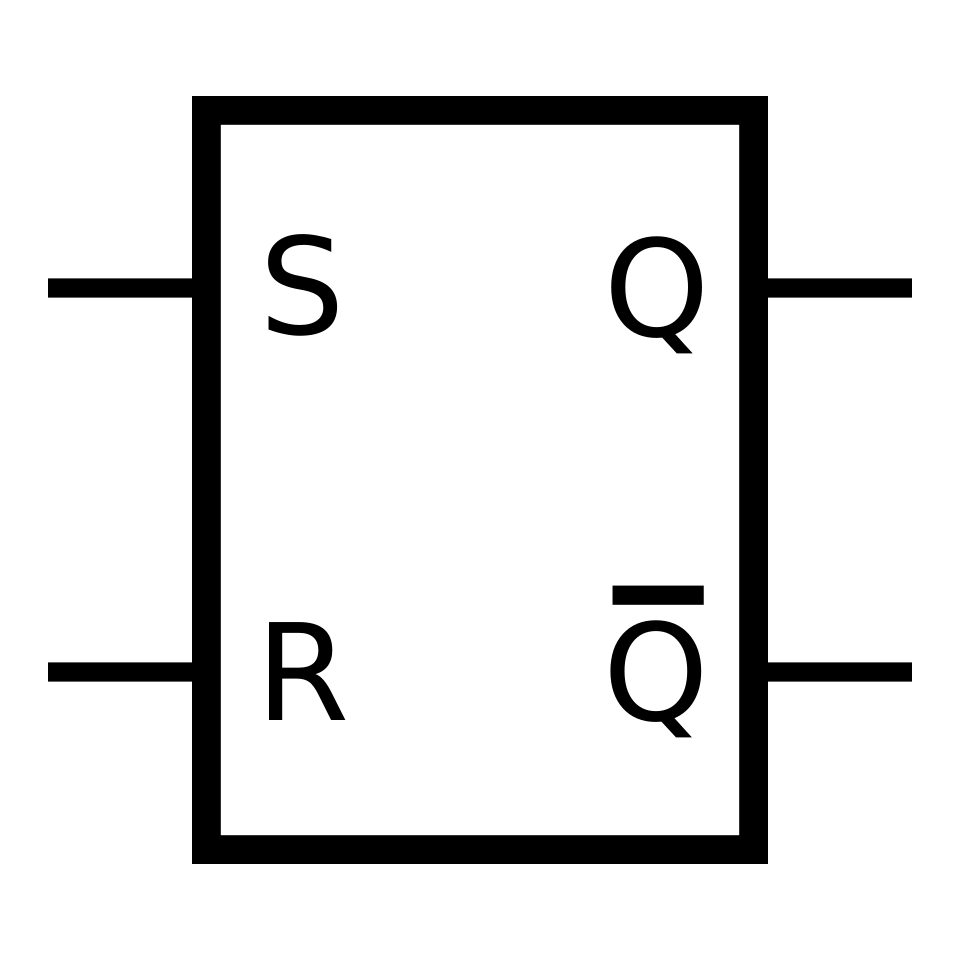
\includegraphics[width=0.15\linewidth,height=\textheight,keepaspectratio]{images/06-sekventiella-kretsar/SR_IEC_symbol.png}

\caption{\label{fig-SR-IEC-symbol}Kretsschemasymbol (IEC) för en
SR-latch med Set och Reset aktivt höga Källa: Av jjbeard - Own Drawing
in Inkscape 0.43, Public Domain,
https://commons.wikimedia.org/w/index.php?curid=873595}

\end{figure}%

\subsection{D-latchen (Data latch)}\label{d-latchen-data-latch}

Som vi sett så har SR-vippan en del egenskaper som kan ge problem. Dels
har den förbjudet tillstånd och som en föjd av detta finns det risk för
kapplöpning och metastabilitet. Dessutom så kommer utgången \(Q\) hela
tiden följa det som händer med Set \(S\) och Reset \(R\). Om SR-vippan
ligger i sin minnesfas med \(S = 1\), så kan en kort, oönskad störning
och spänningsförändring på \(R\) göra så att SR-vippan nollställs.

Det senare problemet kan hanteras genom att lägga till en
\textbf{Enable}. Detta kan implementeras genom att lägga till två
NAND-grindar till den enkla SR-latchen implementerad med NAND, se
Figur~\ref{fig-SR-latch-with-Enable} De extra NAND-grindarna kan öppna
och stänga SR-latchens funktion.

\begin{figure}

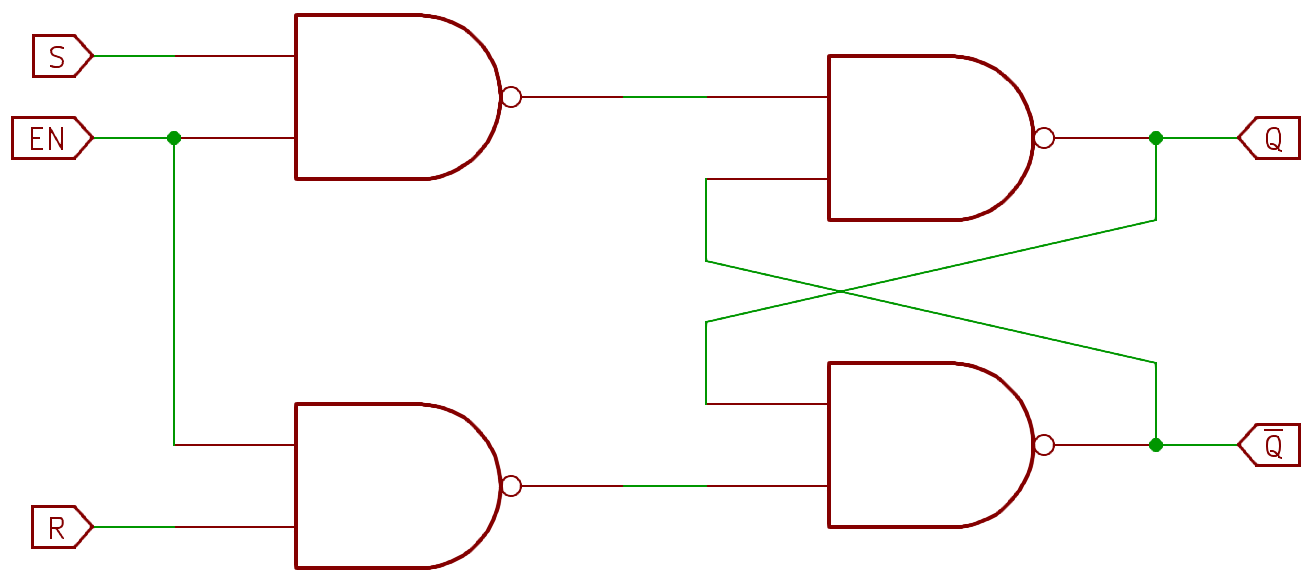
\includegraphics[width=0.5\linewidth,height=\textheight,keepaspectratio]{images/06-sekventiella-kretsar/SR_latch_with_Enable.png}

\caption{\label{fig-SR-latch-with-Enable}SR-latch med Enable (\(EN\))
uppbyggd av två NAND-grindar.}

\end{figure}%

Fast det löser inte problemet med det förbjudna tillståndet! Men med
ytterligare en modifiering av SR-latchen (en inverterare läggs till) så
fås det som heter D-latch (D står för Data). Ingången \(D\) ersätter
\(S\) och \(R\) enligt Figur~\ref{fig-D-latch}. Enable \(EN\) kallas
ofta för \(C\) för en D-latch, där \(C\) står för Control eller Clock.
För att undvika det förbjudna tillståndet i SR-latchen och kontrollera
\emph{när} data ska sparas använder vi en \textbf{D-latch}. Den har en
dataingång (\(D\)) och en aktiveringssignal \(C\).

\begin{figure}

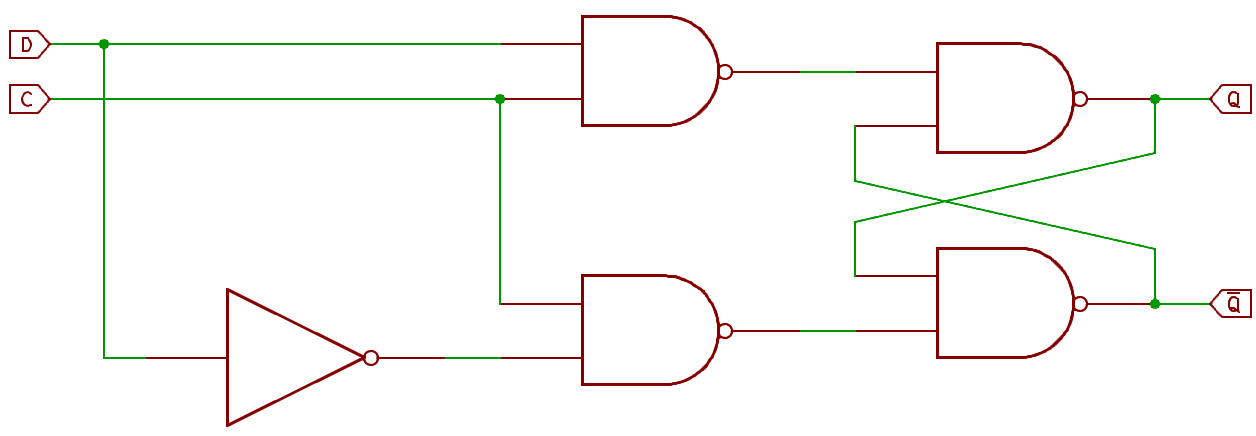
\includegraphics[width=0.5\linewidth,height=\textheight,keepaspectratio]{images/06-sekventiella-kretsar/D_latch.png}

\caption{\label{fig-D-latch}D-latch. Inverteraren gör att ingångarna
till det som är SR-latch med enable inte kommer ha samma värde, mer än
under den korta tidsfördröjning som inverteraren har för att ändra
utsignalen.}

\end{figure}%

Inverteraren gör att problemet med det förbjudna tillståndet elimineras.
Ingångarna till latchen kan inte längre ha samma värde, eftersom de är
inversen av varandra. Sanningstabellen blir också enklare, se
Tabell~\ref{tbl-D-latch}.

\begin{longtable}[]{@{}cccl@{}}
\caption{Sanningstabell för D-latch.}\label{tbl-D-latch}\tabularnewline
\toprule\noalign{}
C & D & \(Q_{n+1}\) & Kommentar \\
\midrule\noalign{}
\endfirsthead
\toprule\noalign{}
C & D & \(Q_{n+1}\) & Kommentar \\
\midrule\noalign{}
\endhead
\bottomrule\noalign{}
\endlastfoot
0 & X & \(Q_0\) & Låst (Behåller tidigare värde) \\
1 & 0 & 0 & Genomskinlig (Reset) \\
1 & 1 & 1 & Genomskinlig (Set) \\
\end{longtable}

\begin{tcolorbox}[enhanced jigsaw, arc=.35mm, bottomrule=.15mm, bottomtitle=1mm, breakable, colback=white, colbacktitle=quarto-callout-note-color!10!white, colframe=quarto-callout-note-color-frame, coltitle=black, left=2mm, leftrule=.75mm, opacityback=0, opacitybacktitle=0.6, rightrule=.15mm, title=\textcolor{quarto-callout-note-color}{\faInfo}\hspace{0.5em}{Praktiskt exempel: Adress-latchning (spara pinnar vid
parallellkommunikation)}, titlerule=0mm, toprule=.15mm, toptitle=1mm]

I mindre inbyggda system eller vid kommunikation med externa minnen vill
man ofta hålla nere antalet anslutningspinnar på processorn för att
spara plats och kostnad. Ett sätt att göra detta är att använda
gemensamma samma pinnar för både \textbf{adress} (var data ska hämtas)
och \textbf{data} (vad som ska hämtas). Detta kallas
Adress/Data-multiplexering.

Här spelar en D-latch (t.ex. den klassiska kretsen 74HC373) en avgörande
roll. Denna krets en en 20-pinnars krets med åtta D-latchar, \(LE\)
(latch enable, kopplad till latchens C-ingång) på ingångssidan och
\(\overline{OE}\) (output eneble) på utgångssidan.

\begin{enumerate}
\def\labelenumi{\arabic{enumi}.}
\tightlist
\item
  \textbf{Adressfas:} Processorn lägger ut adressen på de gemensamma
  pinnarna och sätter kontrollsignalen \(LE\) (i detta sammanhang ofta
  kallad \emph{Address Latch Enable}, ALE) hög. D-latchen blir då
  ``genomskinlig'' och släpper igenom adressen till minneskretsen.
\item
  \textbf{Låsning:} Processorn sätter \(C\) låg (\(0\)). Nu är adressen
  ``fryst'' på latchens utgångar och hålls kvar stabilt mot minnet.
  Latchens utgångar är kopplade till adressbussen, där övriga enheter
  kan läsa vilken adress processorn ska arbeta med.
\item
  \textbf{Datafas:} Processorn kan nu slå om sina egna pinnar och
  använda dem för att läsa in själva datan från minnet (eller skriva),
  utan att adressen försvinner.
\end{enumerate}

Utan D-latchen skulle adressen försvinna så fort processorn slutade
driva den, och minnet skulle inte veta varifrån det ska hämta
informationen.

\end{tcolorbox}

\subsection{Varför räcker inte
latchar?}\label{varfuxf6r-ruxe4cker-inte-latchar}

D-latchen är fortfarande en transparent latch. När \(C = 1\) är latchen
öppen och \(Q = D\), det vill säga data ``slinker igenom'' latchen. Så
om \(D\) ändras under den tid som \(C\) är hög kommer även \(Q\) att
ändras. Det kan vara en oönskad egenskap i vissa system, där man önskar
arbeta synkront med många latchar på ett sådant sätt att utgångsvärdena
sätts vid en distinkt tidpunkt. I komplexa processorer och synkrona
system vill vi att alla delar ska uppdateras exakt samtidigt, som på ett
givet kommando, och inte tillåts variera då kontrollsignalen är aktiv.
Man önskar en digital krets som reagerar på en \textbf{klockflank}. Det
är här klocksignalen och \textbf{Flip-flops} (vippor) kommer in i
bilden. De reagerar bara och låser data på en snabb förändring istället
och kräver inte en stabil nivå under en längre tid.

\section{Vippor (Flip-Flops)}\label{sec-vippor}

Som avsnittet om latchar visade kan det finnas ett inneboende problem
med att de är ``transparenta''. Så länge kontrollsignalen (\(C\)) är
aktiv, kan data flöda fritt genom kretsen. I komplexa system där
tusentals bitar ska flyttas samtidigt i takt med en klocka, skapar detta
osäkerhet och risk för logiska fel.

Lösningen är vippan (flip-flop). Till skillnad från latchen, som
reagerar på en nivå (hög eller låg signal), reagerar vippan endast på en
förändring -- en så kallad flank. Detta kallas för flanktriggning och är
fundamentet för all modern processorarkitektur. Det är detta som gör att
vi kan tala om en processors ``klockfrekvens''; det är takten på dessa
flanker som bestämmer när hela systemet tar nästa steg i sina
beräkningar.

\subsection{Triggningsmetoder: Positiv och negativ
flanktriggning}\label{triggningsmetoder-positiv-och-negativ-flanktriggning}

En klocksignal är i grunden en fyrkantsvåg som växlar mellan logisk 0
och 1. En vippa är konstruerad för att ``sampla'' (läsa av) sin ingång
exakt i det ögonblick då klocksignalen byter tillstånd. Det finns två
huvudsakliga sätt att trigga en vippa:

Positiv flanktriggning (Stigande flank): Vippan reagerar exakt när
klocksignalen går från 0 till 1. Detta är den absolut vanligaste metoden
i modern digitalteknik. I kretsscheman ritas detta med en liten triangel
vid klocksingången.

Negativ flanktriggning (Fallande flank): Vippan reagerar istället när
klocksignalen går från 1 till 0. I kretsscheman markeras detta med en
liten ring (invertering) framför triangeln vid klocksingången.

\begin{tcolorbox}[enhanced jigsaw, arc=.35mm, bottomrule=.15mm, bottomtitle=1mm, breakable, colback=white, colbacktitle=quarto-callout-tip-color!10!white, colframe=quarto-callout-tip-color-frame, coltitle=black, left=2mm, leftrule=.75mm, opacityback=0, opacitybacktitle=0.6, rightrule=.15mm, title=\textcolor{quarto-callout-tip-color}{\faLightbulb}\hspace{0.5em}{Tips}, titlerule=0mm, toprule=.15mm, toptitle=1mm]

Varför är flanken så viktig? Tänk på en vippa som en kamera. En latch
fungerar som en videokamera som spelar in allt så länge knappen är
intryckt. En vippa fungerar däremot som en stillbildskamera: den tar ett
``foto'' av ingången exakt vid flanken. Vad som händer med ingången
precis före eller precis efter flanken spelar ingen roll -- det är bara
bilden som togs i klockögonblicket som sparas i minnet.

\end{tcolorbox}

Detta korta ögonblick av sampling gör att vi kan koppla samman
miljontals vippor i långa kedjor. Eftersom de bara ändrar sig vid
flanken, riskerar vi inte att data ``rinner igenom'' flera steg under en
och samma klockcykel, vilket är en förutsättning för att kunna bygga
fungerande datorer.

\subsection{D-vippan (Edge-triggered D
Flip-Flop)}\label{d-vippan-edge-triggered-d-flip-flop}

D-vippan är den absolut viktigaste byggstenen i modern digitalteknik.
Nästan alla register i en processor, från enkla statusflaggor till breda
databussar, består av rader med D-vippor.

Namnet ``D'' står för \textbf{Data} (eller ibland \emph{Delay}), och
precis som för D-latchen är funktionen enkel: utgången \(Q\) ska kopiera
värdet på ingången \(D\). Skillnaden ligger i \emph{när} detta sker.
Medan latchen är öppen så länge kontrollsignalen är hög, läser vippan av
\(D\) endast vid en \textbf{klockflank}.

För att skapa denna ``ögonblicksbild'' (sampling) internt, kopplar man
oftast samman två D-latchar i serie. Denna konstruktion kallas för en
\textbf{Master-Slave}-konfiguration, se
\textbf{?@fig-fig-D-flipflop-logic}.

\begin{enumerate}
\def\labelenumi{\arabic{enumi}.}
\tightlist
\item
  \textbf{Master-latchen} är öppen när klockan är låg (på grund av den
  första inverteringen av \(C\)). Den följer ingången \(D\) men kan inte
  nå utgången \(Q\) på vippan än.
\item
  \textbf{Slave-latchen} är låst när klockan är låg, vilket gör att
  utgången \(Q\) behåller sitt gamla värde.
\item
  \textbf{Vid flanken (0 till 1):} Master-latchen låser sig (fryser
  värdet på \(D\)), samtidigt som Slave-latchen öppnas och skickar ut
  det frysta värdet till \(Q\).
\end{enumerate}

Resultatet blir att utgången endast kan ändras exakt vid den stigande
flanken.

\begin{figure}

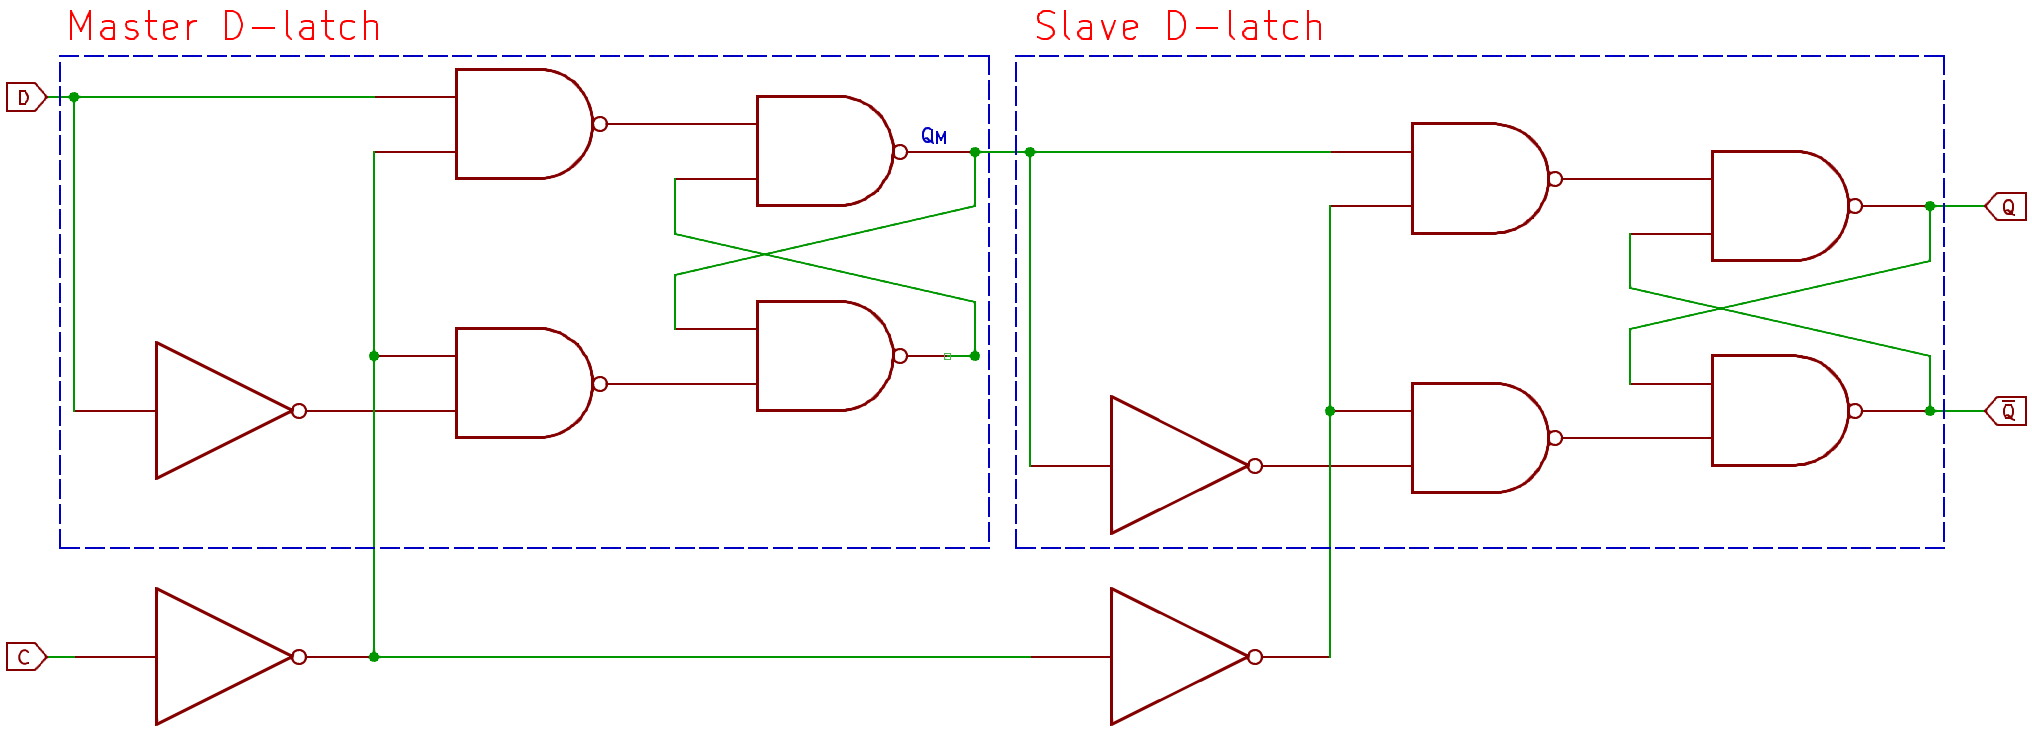
\includegraphics[width=0.7\linewidth,height=\textheight,keepaspectratio]{images/06-sekventiella-kretsar/D_flipflop_master_slave.png}

\caption{\label{fig-D-flipflop-logic}Intern uppbyggnad av en D-vippa
enligt Master-Slave-principen. Inverteraren ser till att de två
latcharna aldrig är öppna samtidigt.}

\end{figure}%

I sanningstabellen för en vippa använder vi en pil (\(\uparrow\)) för
att markera den stigande klockflanken. Detta skiljer den tydligt från
latcharnas tabeller där vi använde logiska nivåer (0 eller 1).

\begin{longtable}[]{@{}
  >{\centering\arraybackslash}p{(\linewidth - 8\tabcolsep) * \real{0.2083}}
  >{\centering\arraybackslash}p{(\linewidth - 8\tabcolsep) * \real{0.2083}}
  >{\centering\arraybackslash}p{(\linewidth - 8\tabcolsep) * \real{0.2083}}
  >{\centering\arraybackslash}p{(\linewidth - 8\tabcolsep) * \real{0.2083}}
  >{\raggedright\arraybackslash}p{(\linewidth - 8\tabcolsep) * \real{0.1667}}@{}}
\caption{Sanningstabell för positivt flanktriggad
D-vippa.}\label{tbl-D-flipflop}\tabularnewline
\toprule\noalign{}
\begin{minipage}[b]{\linewidth}\centering
C
\end{minipage} & \begin{minipage}[b]{\linewidth}\centering
D
\end{minipage} & \begin{minipage}[b]{\linewidth}\centering
\(Q\)
\end{minipage} & \begin{minipage}[b]{\linewidth}\centering
\(\overline{Q}\)
\end{minipage} & \begin{minipage}[b]{\linewidth}\raggedright
Kommentar
\end{minipage} \\
\midrule\noalign{}
\endfirsthead
\toprule\noalign{}
\begin{minipage}[b]{\linewidth}\centering
C
\end{minipage} & \begin{minipage}[b]{\linewidth}\centering
D
\end{minipage} & \begin{minipage}[b]{\linewidth}\centering
\(Q\)
\end{minipage} & \begin{minipage}[b]{\linewidth}\centering
\(\overline{Q}\)
\end{minipage} & \begin{minipage}[b]{\linewidth}\raggedright
Kommentar
\end{minipage} \\
\midrule\noalign{}
\endhead
\bottomrule\noalign{}
\endlastfoot
0, 1, \(\downarrow\) & X & \(Q_0\) & \(\overline{Q_0}\) & \textbf{Vila:}
Ingen ändring sker utom vid stigande flank. \\
\(\uparrow\) & 0 & 0 & 1 & \textbf{Sampling:} En nolla sparas på
flanken. \\
\(\uparrow\) & 1 & 1 & 0 & \textbf{Sampling:} En etta sparas på
flanken. \\
\end{longtable}

Sanningstabellen visar inte fullt ut hur funktionen i en D-vippa skiljer
sig från funktionen i en D-latch. Då är timingdiagrammet ett bättre
verktyg. I Figur~\ref{fig-timing-dff} ser vi hur en vippa reagerar på
insignaler. Till skillnad från D-latchen, som är ``genomskinlig'',
påverkas inte vippans utgång av vad som händer med \(D\) mellan
klockflankerna. Det är endast värdet precis vid pilen (\(\uparrow\)) som
spelar roll. Men i signalen \(Q_M\) som ligger mellan Master-latchen och
Slave-latchen syns att första halvan av D-vippan är transparent.

\begin{figure}

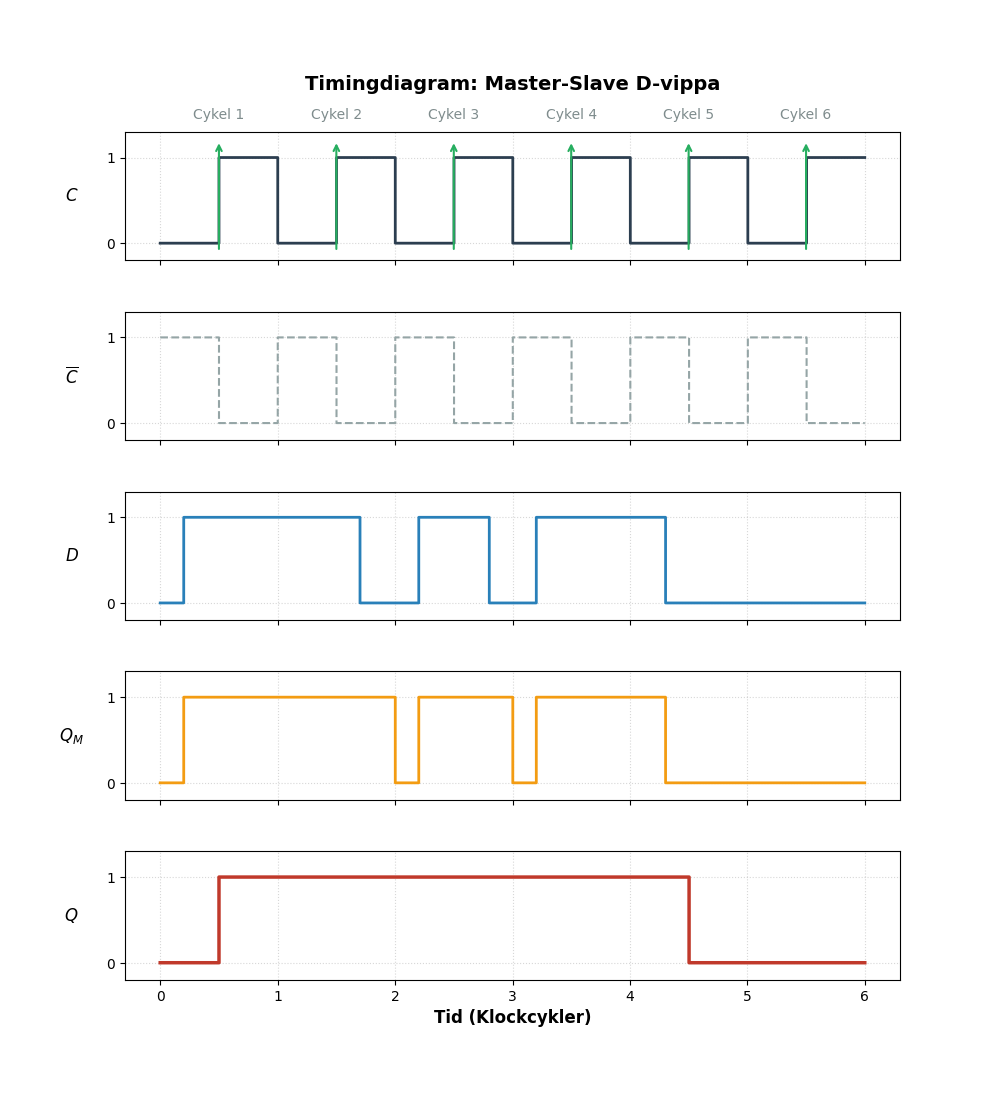
\includegraphics[width=0.7\linewidth,height=\textheight,keepaspectratio]{images/06-sekventiella-kretsar/timing_dff.png}

\caption{\label{fig-timing-dff}Timingdiagram för en D-vippa.
Master-latchen aktiveras och blir transparent vid låg klocksignal
(\(Q_M\)). Samtidigt så är Slave-latchen låst. När klockan slår om från
låg till hög (positiv flank) låses Master-latchen och dess utsignal
sätter utgången Q}

\end{figure}%

\begin{tcolorbox}[enhanced jigsaw, arc=.35mm, bottomrule=.15mm, bottomtitle=1mm, breakable, colback=white, colbacktitle=quarto-callout-important-color!10!white, colframe=quarto-callout-important-color-frame, coltitle=black, left=2mm, leftrule=.75mm, opacityback=0, opacitybacktitle=0.6, rightrule=.15mm, title=\textcolor{quarto-callout-important-color}{\faExclamation}\hspace{0.5em}{Setup och Hold time}, titlerule=0mm, toprule=.15mm, toptitle=1mm]

Eftersom en vippa samplar data precis vid en flank, finns det fysiska
krav på insignalen \(D\) för att undvika fel: * \textbf{Setup time
(\(t_s\)):} Data måste ha varit stabil en kort stund \emph{innan}
flanken kommer. * \textbf{Hold time (\(t_h\)):} Data måste ligga kvar en
kort stund \emph{efter} att flanken passerat.

Om dessa tider inte respekteras (till exempel om \(D\) ändras precis
samtidigt som klockan slår) riskerar vippan att hamna i
\textbf{metastabilitet}, där utgången under en tid hamnar i ett obestämt
läge mellan 0 och 1.

\end{tcolorbox}

\subsection{JK-vippan - den universella
vippan}\label{jk-vippan---den-universella-vippan}

\subsection{JK-vippan -- den universella
vippan}\label{jk-vippan-den-universella-vippan}

JK-vippan kan ses som en vidareutveckling av den enkla SR-latchen, men
med två avgörande skillnader: den är \textbf{flanktriggad} och den har
inget ``förbjudet'' tillstånd. Namnet kommer enligt legenden från Jack
Kilby, uppfinnaren av den integrerade kretsen.

Ingångarna \(J\) (Jump/Set) och \(K\) (Kill/Reset) fungerar analogt med
Set och Reset, men med en unik twist när båda är höga samtidigt.

\subsubsection{Sanningstabell}\label{sanningstabell}

Det som gör JK-vippan unik är raden där både \(J\) och \(K\) är 1.
Istället för att hamna i ett ogiltigt läge, kommer vippan att
\textbf{toggla} (växla tillstånd). Om utgången var 0 blir den 1, och
vice versa.

\begin{longtable}[]{@{}
  >{\centering\arraybackslash}p{(\linewidth - 8\tabcolsep) * \real{0.2083}}
  >{\centering\arraybackslash}p{(\linewidth - 8\tabcolsep) * \real{0.2083}}
  >{\centering\arraybackslash}p{(\linewidth - 8\tabcolsep) * \real{0.2083}}
  >{\centering\arraybackslash}p{(\linewidth - 8\tabcolsep) * \real{0.2083}}
  >{\raggedright\arraybackslash}p{(\linewidth - 8\tabcolsep) * \real{0.1667}}@{}}
\caption{Sanningstabell för positivt flanktriggad
JK-vippa.}\label{tbl-JK-flipflop}\tabularnewline
\toprule\noalign{}
\begin{minipage}[b]{\linewidth}\centering
C
\end{minipage} & \begin{minipage}[b]{\linewidth}\centering
J
\end{minipage} & \begin{minipage}[b]{\linewidth}\centering
K
\end{minipage} & \begin{minipage}[b]{\linewidth}\centering
\(Q\)
\end{minipage} & \begin{minipage}[b]{\linewidth}\raggedright
Kommentar
\end{minipage} \\
\midrule\noalign{}
\endfirsthead
\toprule\noalign{}
\begin{minipage}[b]{\linewidth}\centering
C
\end{minipage} & \begin{minipage}[b]{\linewidth}\centering
J
\end{minipage} & \begin{minipage}[b]{\linewidth}\centering
K
\end{minipage} & \begin{minipage}[b]{\linewidth}\centering
\(Q\)
\end{minipage} & \begin{minipage}[b]{\linewidth}\raggedright
Kommentar
\end{minipage} \\
\midrule\noalign{}
\endhead
\bottomrule\noalign{}
\endlastfoot
\(\uparrow\) & 0 & 0 & \(Q_0\) & \textbf{Minne:} Ingen ändring sker. \\
\(\uparrow\) & 0 & 1 & 0 & \textbf{Reset:} Utgången nollställs. \\
\(\uparrow\) & 1 & 0 & 1 & \textbf{Set:} Utgången sätts till ett. \\
\(\uparrow\) & 1 & 1 & \(\overline{Q_0}\) & \textbf{Toggle:} Utgången
byter tillstånd (0→1 eller 1→0). \\
\end{longtable}

\subsubsection{Varför är JK-vippan
``universell''?}\label{varfuxf6r-uxe4r-jk-vippan-universell}

Anledningen till att JK-vippan ofta kallas universell är att den enkelt
kan konfigureras för att utföra andra vippors jobb: * \textbf{Som en
D-vippa:} Koppla en inverterare mellan \(J\) och \(K\) och använd \(J\)
som dataingång. * \textbf{Som en T-vippa:} Koppla ihop \(J\) och \(K\)
till en gemensam ingång.

\subsubsection{Intern logik och
återkoppling}\label{intern-logik-och-uxe5terkoppling}

JK-vippan löser SR-latchens problem med det förbjudna tillståndet genom
att internt återkoppla utgångarna till ingångsgrindarna. Om utgången
\(Q\) redan är 1, kommer ``Set''-ingången (\(J\)) att spärras logiskt,
vilket gör att endast en ``Reset''-operation (eller en toggle) är
möjlig.

\pandocbounded{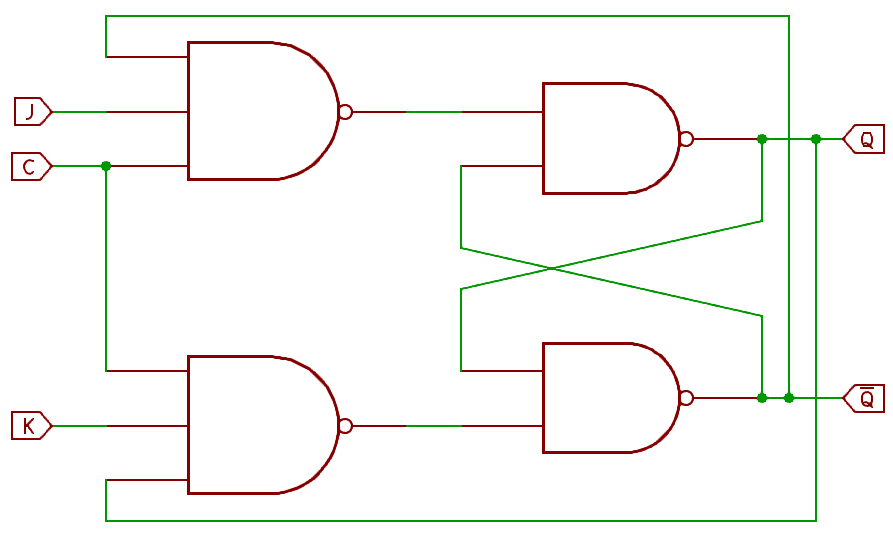
\includegraphics[keepaspectratio,alt={Logiskt schema för en JK-vippa. Notera återkopplingen från utgångarna tillbaka till ingångsgrindarna som möjliggör toggle-funktionen.}]{images/06-sekventiella-kretsar/JK_flipflop_logic.png}}\{\#fig-JK-logic

\subsection{T-vippan - toogle-vippan för
räknare}\label{t-vippan---toogle-vippan-fuxf6r-ruxe4knare}

\subsection{T-vippan -- toggle-vippan för
räknare}\label{t-vippan-toggle-vippan-fuxf6r-ruxe4knare}

T-vippan (där T står för \textbf{Toggle}) har bara en enda dataingång.
Dess enda uppgift är att hålla reda på om den ska behålla sitt nuvarande
värde eller ``slå om'' (invertera) vid nästa klockflank.

Detta gör den till hjärtat i nästan alla digitala räknare och
klockfrekvensdelare.

\subsubsection{Funktion och
Sanningstabell}\label{funktion-och-sanningstabell}

Logiken är extremt rak: * Om \(T=0\), händer ingenting vid klockflanken
(\textbf{Minne}). * Om \(T=1\), byter utgången tillstånd vid
klockflanken (\textbf{Toggle}).

\begin{longtable}[]{@{}
  >{\centering\arraybackslash}p{(\linewidth - 6\tabcolsep) * \real{0.2632}}
  >{\centering\arraybackslash}p{(\linewidth - 6\tabcolsep) * \real{0.2632}}
  >{\centering\arraybackslash}p{(\linewidth - 6\tabcolsep) * \real{0.2632}}
  >{\raggedright\arraybackslash}p{(\linewidth - 6\tabcolsep) * \real{0.2105}}@{}}
\caption{Sanningstabell för positivt flanktriggad
T-vippa.}\label{tbl-T-flipflop}\tabularnewline
\toprule\noalign{}
\begin{minipage}[b]{\linewidth}\centering
C
\end{minipage} & \begin{minipage}[b]{\linewidth}\centering
T
\end{minipage} & \begin{minipage}[b]{\linewidth}\centering
\(Q\)
\end{minipage} & \begin{minipage}[b]{\linewidth}\raggedright
Kommentar
\end{minipage} \\
\midrule\noalign{}
\endfirsthead
\toprule\noalign{}
\begin{minipage}[b]{\linewidth}\centering
C
\end{minipage} & \begin{minipage}[b]{\linewidth}\centering
T
\end{minipage} & \begin{minipage}[b]{\linewidth}\centering
\(Q\)
\end{minipage} & \begin{minipage}[b]{\linewidth}\raggedright
Kommentar
\end{minipage} \\
\midrule\noalign{}
\endhead
\bottomrule\noalign{}
\endlastfoot
\(\uparrow\) & 0 & \(Q_0\) & \textbf{Minne:} Utgången förblir
oförändrad. \\
\(\uparrow\) & 1 & \(\overline{Q_0}\) & \textbf{Toggle:} Utgången
inverteras (0→1 eller 1→0). \\
\end{longtable}

\subsubsection{T-vippan som
frekvensdelare}\label{t-vippan-som-frekvensdelare}

En av de vanligaste applikationerna för en T-vippa är att dela en
klockfrekvens med två. Om man kopplar \(T\) permanent till logisk etta
(\(1\)), kommer utgången \(Q\) att växla vid varje klockflank.

Det innebär att \(Q\) går hög vid första flanken, låg vid andra, hög vid
tredje, och så vidare. Resultatet blir en ny fyrkantsvåg på utgången som
har exakt \textbf{hälften} så hög frekvens som den ursprungliga
klocksignalen. Genom att kedjekoppla flera T-vippor kan man enkelt dela
ner en hög klockfrekvens till lägre hastigheter eller bygga binära
räknare.

\begin{figure}

\includegraphics[width=0.8\linewidth,height=\textheight,keepaspectratio]{images/06-sekventiella-kretsar/T_flipflop_timing.png}

\caption{\label{fig-T-timing}Timingdiagram för en T-vippa med T=1.
Notera hur utgången Q ändrar tillstånd vid varje stigande klockflank,
vilket resulterar i en halvering av frekvensen.}

\end{figure}%

\subsubsection{Implementering}\label{implementering}

I praktiken köper man sällan en ren ``T-vippa'' som en enskild krets.
Istället skapar man den genom att använda en \textbf{JK-vippa} där man
kopplar samman \(J\) och \(K\) till en gemensam \(T\)-ingång, eller en
\textbf{D-vippa} där man återkopplar den inverterade utgången
\(\overline{Q}\) till \(D\)-ingången.

\begin{tcolorbox}[enhanced jigsaw, arc=.35mm, bottomrule=.15mm, bottomtitle=1mm, breakable, colback=white, colbacktitle=quarto-callout-tip-color!10!white, colframe=quarto-callout-tip-color-frame, coltitle=black, left=2mm, leftrule=.75mm, opacityback=0, opacitybacktitle=0.6, rightrule=.15mm, title=\textcolor{quarto-callout-tip-color}{\faLightbulb}\hspace{0.5em}{Kom ihåg regeln}, titlerule=0mm, toprule=.15mm, toptitle=1mm]

Tänk på T-vippan som en strömbrytare med en tryckknapp: * \(T=0\): Du
trycker inte på knappen (lampan förblir som den är). * \(T=1\): Du
trycker på knappen vid varje klockslag (lampan tänds/släcks varje gång).

\end{tcolorbox}

\subsection{Asynkrona ingångar för vippor (Preset och
Clear)}\label{asynkrona-inguxe5ngar-fuxf6r-vippor-preset-och-clear}

\subsection{Asynkrona ingångar för vippor (Preset och
Clear)}\label{asynkrona-inguxe5ngar-fuxf6r-vippor-preset-och-clear-1}

Hittills har vi bara tittat på \textbf{synkrona} ingångar
(\(D, J, K, T\)), vilket innebär att vippan endast bryr sig om dem exakt
vid klockflanken. Men i verkliga system behöver vi ibland kunna styra
vippan omedelbart, oavsett vad klockan gör.

För detta använder vi \textbf{asynkrona ingångar}, oftast kallade
\textbf{Preset} (Sätt till 1) och \textbf{Clear} (Nollställ). Dessa
ingångar har ``högsta prioritet'' och kör över allt annat.

\subsubsection{\texorpdfstring{Preset (\(PRE\)) och Clear
(\(CLR\))}{Preset (PRE) och Clear (CLR)}}\label{preset-pre-och-clear-clr}

\begin{itemize}
\tightlist
\item
  \textbf{Preset:} Tvingar utgången \(Q\) till 1 omedelbart.
\item
  \textbf{Clear:} Tvingar utgången \(Q\) till 0 omedelbart.
\end{itemize}

I de flesta kommersiella kretsar (som t.ex. 74HC74) är dessa ingångar
\textbf{aktivt låga}. Det betyder att de måste dras till 0 för att
aktiveras, vilket i kretsscheman ritas med en liten ring vid ingången
och betecknas med ett streck över namnet (\(\overline{PRE}\) och
\(\overline{CLR}\)).

\subsubsection{Varför behövs asynkrona
ingångar?}\label{varfuxf6r-behuxf6vs-asynkrona-inguxe5ngar}

Den vanligaste användningen är vid \textbf{systemstart}. När strömmen
slås på i en dator eller mikrokontroller kan vipporna hamna i ett
slumpmässigt tillstånd (0 eller 1). Genom att skicka en kort asynkron
``Clear''-puls till alla vippor i hela systemet garanterar man att
maskinen startar från ett definierat nollställt läge.

\subsubsection{Skillnaden mellan synkron och asynkron
nollställning}\label{skillnaden-mellan-synkron-och-asynkron-nollstuxe4llning}

Det är viktigt att förstå skillnaden i ett timingdiagram: 1.
\textbf{Synkron Reset:} Vippan nollställs endast om Reset-signalen är
aktiv \emph{samtidigt} som en klockflank sker. 2. \textbf{Asynkron
Reset:} Vippan nollställs \emph{i samma ögonblick} som Reset-signalen
blir aktiv, helt oberoende av klockan.

\begin{tcolorbox}[enhanced jigsaw, arc=.35mm, bottomrule=.15mm, bottomtitle=1mm, breakable, colback=white, colbacktitle=quarto-callout-warning-color!10!white, colframe=quarto-callout-warning-color-frame, coltitle=black, left=2mm, leftrule=.75mm, opacityback=0, opacitybacktitle=0.6, rightrule=.15mm, title=\textcolor{quarto-callout-warning-color}{\faExclamationTriangle}\hspace{0.5em}{Prioritetsfällan}, titlerule=0mm, toprule=.15mm, toptitle=1mm]

Om både Preset och Clear aktiveras samtidigt hamnar vippan i ett
instabilt eller odefinierat läge (likt det förbjudna tillståndet i en
SR-latch). I normal drift måste man se till att båda dessa ingångar är
inaktiva (oftast hållna höga till logisk 1) för att vippan ska lyda
klockan och dataingångarna.

\end{tcolorbox}

\bookmarksetup{startatroot}

\chapter*{Referenser}\label{referenser}
\addcontentsline{toc}{chapter}{Referenser}

\markboth{Referenser}{Referenser}

\protect\phantomsection\label{refs}

\bookmarksetup{startatroot}

\chapter*{Appendix}\label{appendix}
\addcontentsline{toc}{chapter}{Appendix}

\markboth{Appendix}{Appendix}

\newpage

\section*{ASCII-tabell}\label{sec-ascii}
\addcontentsline{toc}{section}{ASCII-tabell}

\markright{ASCII-tabell}

ASCII - American Standard Code for Information Interchange.

Ursprunget till ASCII är en standardisering av en 7-bitars kod för
teleprinter. Standarden innehåller både styrtecken och skrivbara tecken.
Senare utökades ASCII till 8-bitarsvarianter (så kallad Extended ASCII),
som möjliggjorde representation av ytterligare tecken såsom å, ä och ö.
Denna begränsning i antal tecken ledde i sin tur till utvecklingen av
Unicode, som i dag är den dominerande standarden för att representera
tecken från världens alla skriftsystem.

\begin{figure}

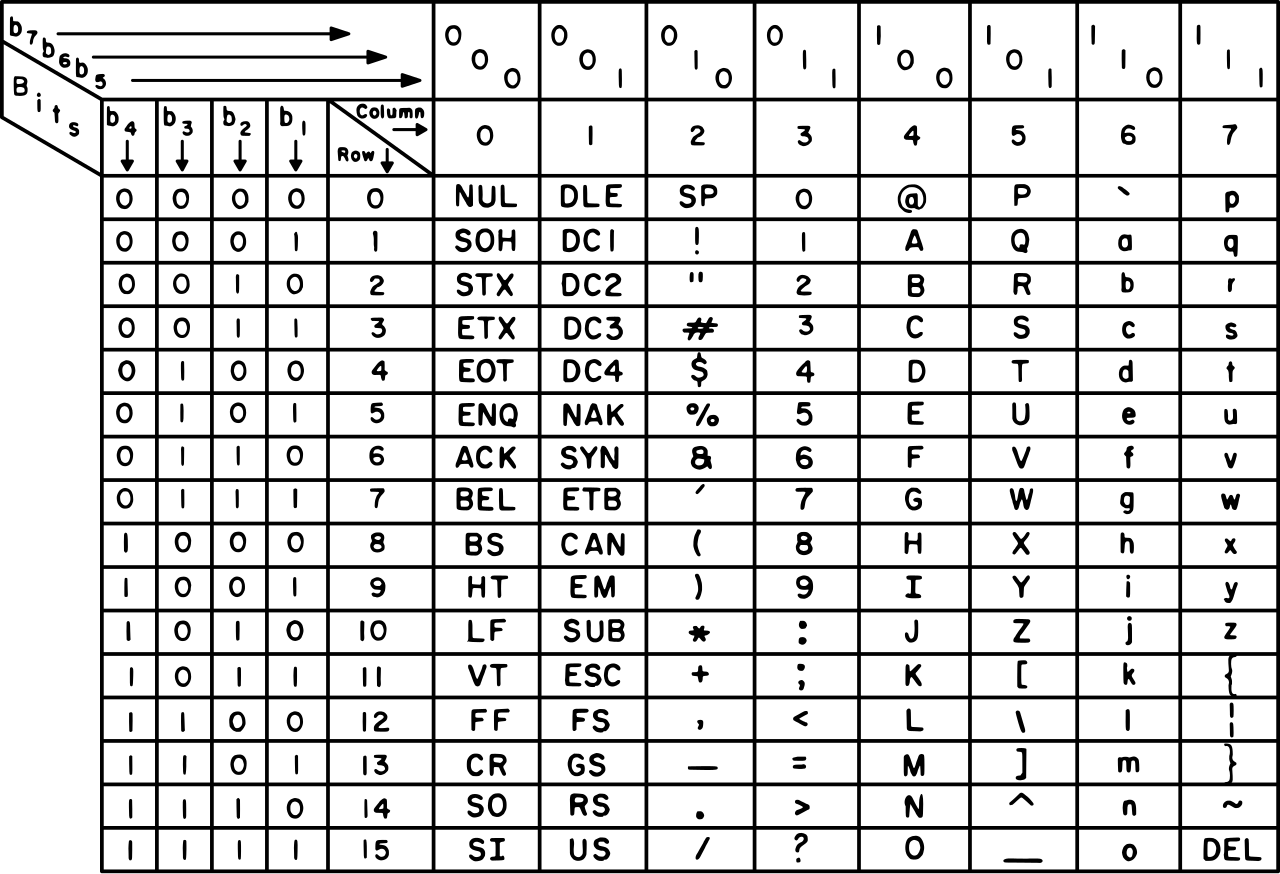
\includegraphics[width=0.8\linewidth,height=\textheight,keepaspectratio]{images/a1-appendix/USASCII_code_chart.png}

\caption{\label{fig-ascii}\textbf{Figurtext:} Fullständig ASCII-tabell.
\emph{Källa: Från Wikipedia, By An unknown officer or employee of the
United States Government - File:USASCII code chart.png, MIL-STD-188-100,
pg. B-2, Fig 1, 1972. (different scan), Public Domain,
https://commons.wikimedia.org/w/index.php?curid=152723332}.}

\end{figure}%

\newpage

\section*{Annat appendix}\label{sec-annat}
\addcontentsline{toc}{section}{Annat appendix}

\markright{Annat appendix}


\backmatter


\end{document}
